\section{Графы}

\subsection{Основные определения}

\textbf{Граф} представляет собой множество \(V\) вершин и набор \(X\) неупорядоченных и упорядоченных пар вершин. Неупорядоченная пара вершин называется \textbf{ребром}, упорядоченная пара --- \textbf{дугой}.

Граф, содержащий только ребра, называется \textbf{неориентированным} и обозначается \(G = (V, X)\). Граф, содержащий только дуги, называется \textbf{ориентированным} (или \textbf{орграфом}) и обозначается \(D = (V, X)\).

Говорят, что ребро \(\{u, v\}\) соединяет вершины \(u\) и \(v\), дуга \((u, v)\) начинается в вершине \(u\) и кончается в вершине \(v\).

Вершины, соединенные ребром или дугой, называются \textbf{смежными}. Ребра, имеющие общую вершину, также называются \textbf{смежными}. Ребро (дуга) и любая из его двух вершин называются \textbf{инцидентными}.

Пара вершин может соединяться двумя или более ребрами (дугами одного направления), такие ребра (дуги) называются \textbf{кратными} (параллельными).

Дуга (ребро) может начинаться и кончаться в одной и той же вершине, такая дуга (ребро) называется \textbf{петлей}.

Граф называется \textbf{простым}, если он не содержит петель и параллельных ребер. В \textbf{мультиграфе} могут быть кратные ребра. В \textbf{псевдографе} допускаются петли и кратные ребра.

\subsection{Порядок графа}

Граф \(G\) является графом порядка \(n\), если множество его вершин \(V\) состоит из \(n\) элементов: \(V = \{v_1, \ldots, v_n\}\).

Граф с \(n\) вершинами и \(m\) ребрами называют \((n, m)\)-графом. Граф, не имеющий ребер, называется \textbf{пустым}. Граф \((1, 0)\) называется \textbf{тривиальным}. Граф, не имеющий вершин, называется \textbf{нуль-графом}.

\subsection{Наглядное представление графа}

Каждый граф можно представить в евклидовом пространстве множеством точек, соответствующих вершинам, которые соединены линиями, соответствующими ребрам (или дугам, если у них указаны направления). Таким образом, граф можно изобразить рисунком, который наглядно изображает некоторую ситуацию.

\begin{example*}
    Задан граф \(G\), состоящий из вершин \(v_1\), \(v_2\), \(v_3\), \(v_4\), \(v_5\), \(v_6\) и ребер \(x_1\), \(x_2\), \(x_3\), \(x_4\), \(x_5\), \(x_6\):
    \begin{gather*}
        x_1 = (v_1, v_2),
        \quad
        x_2 = (v_1, v_4),
        \quad
        x_3 = (v_5, v_6),
        \\
        x_4 = (v_1, v_2),
        \quad
        x_5 = (v_5, v_5).
    \end{gather*}

    \begin{figure}[H]
        \centering
        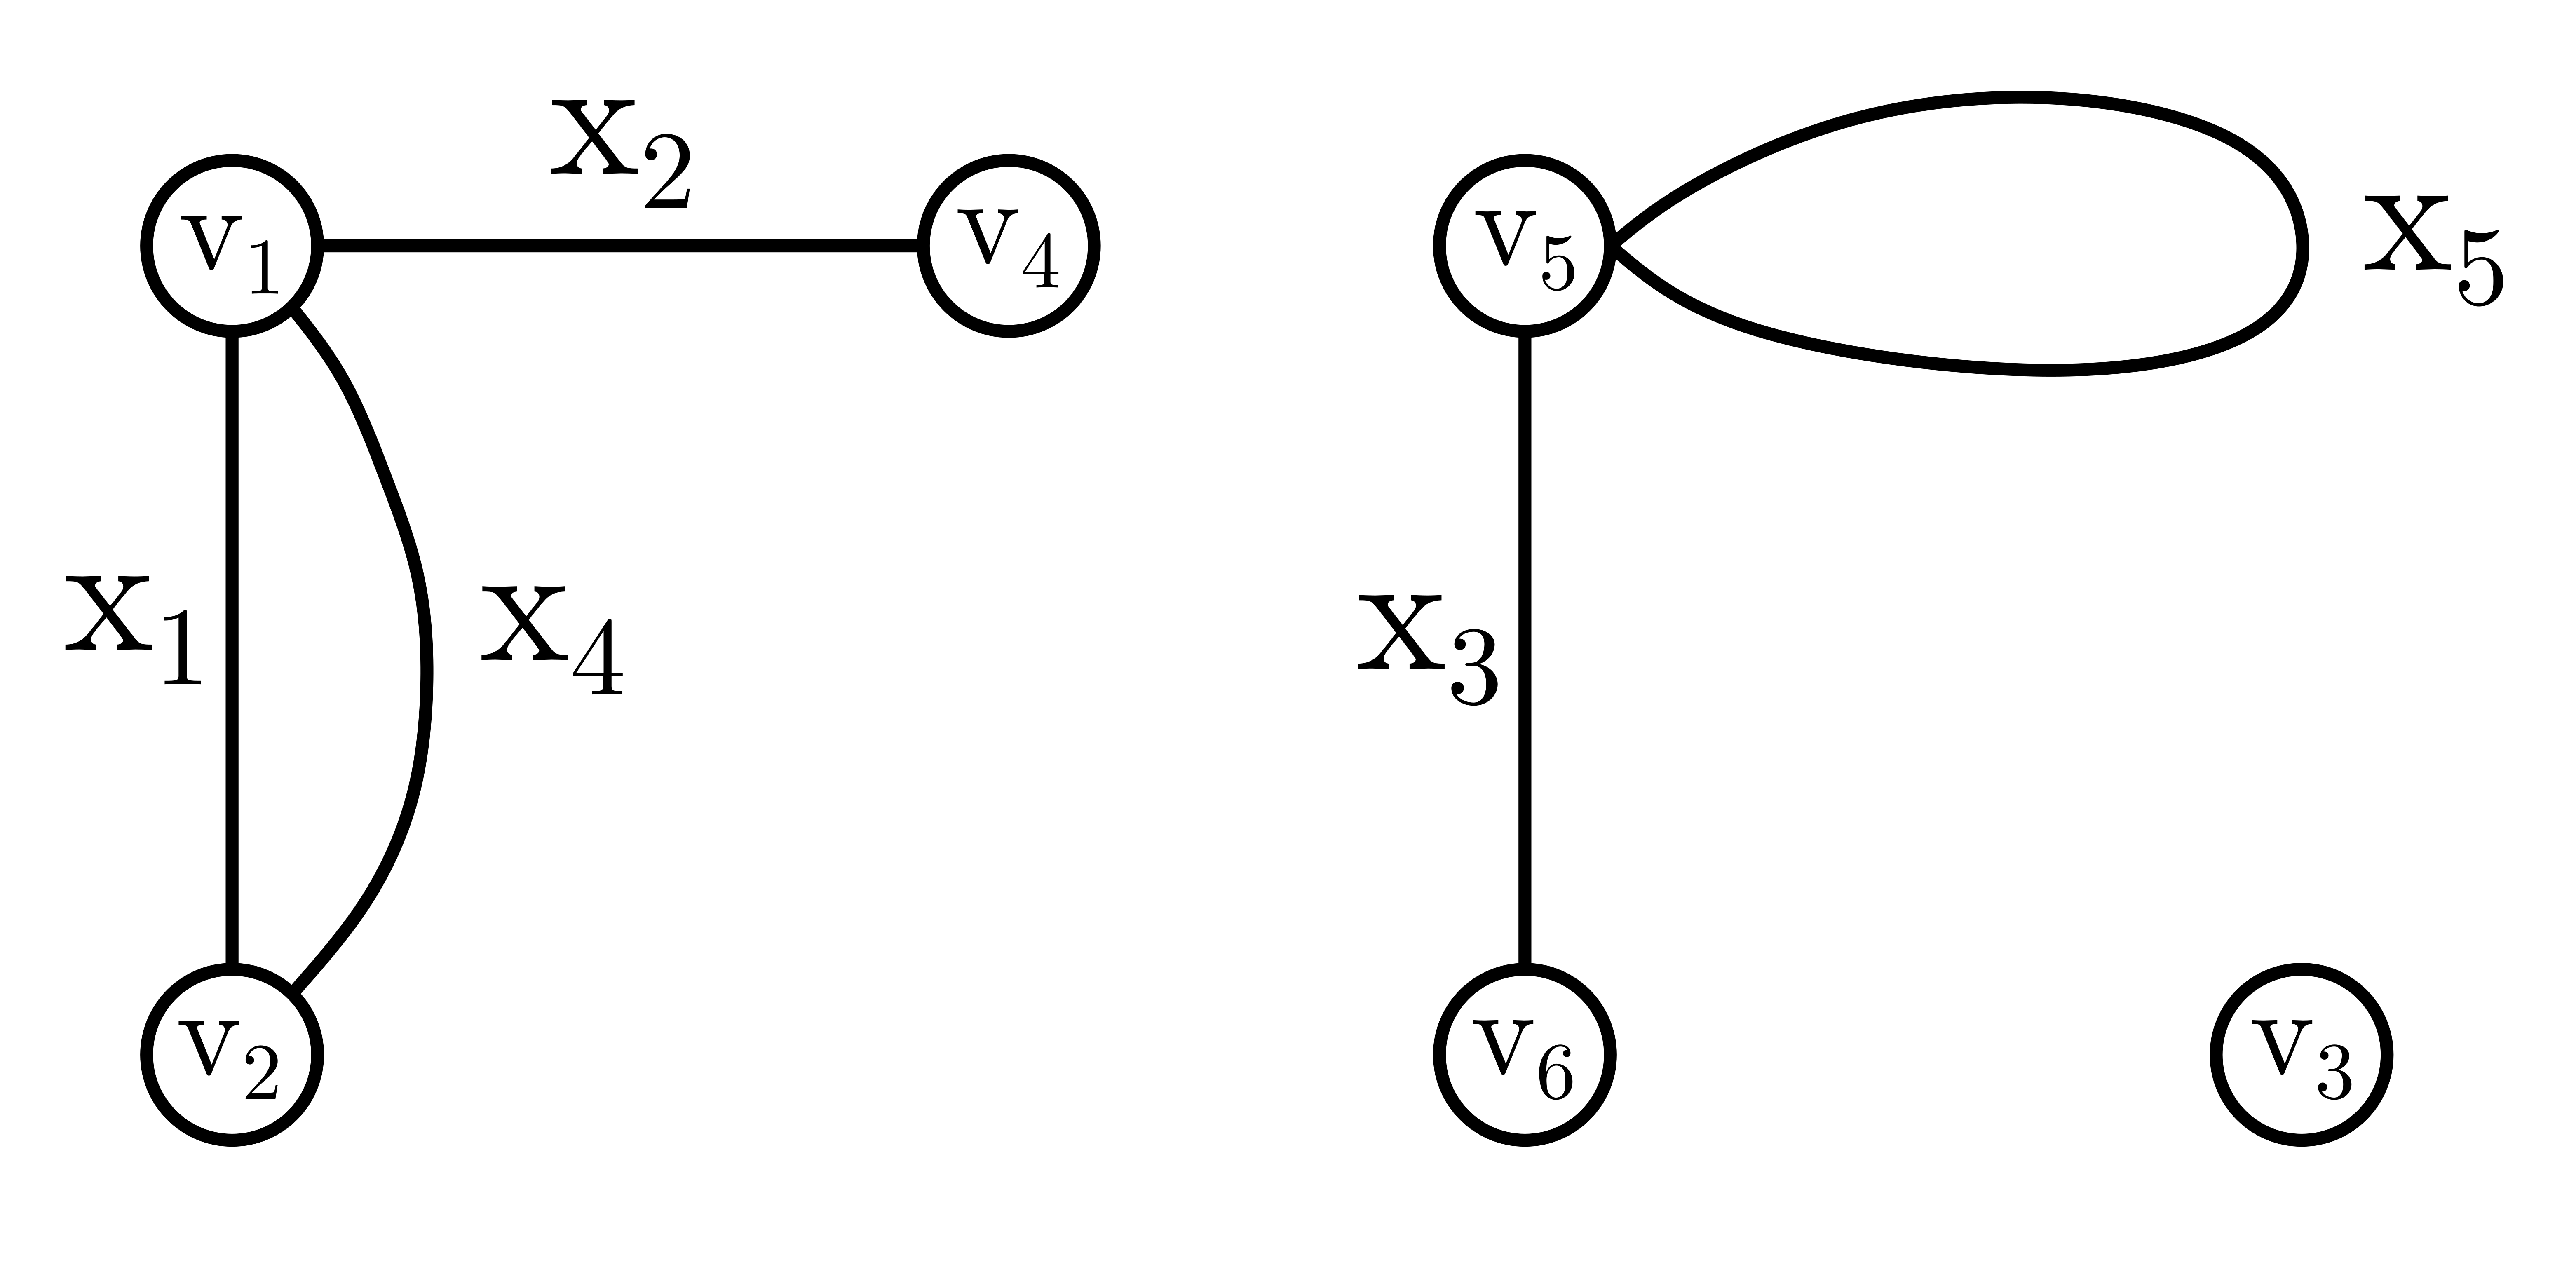
\includegraphics[width=0.8\textwidth]{./images/graph-example.png}
    \end{figure}

    \noindent Проанализировав граф, имеем:
    \begin{itemize}
        \item \(x_1\) и \(x_4\) --- кратные ребра;
        \item \(x_5\) --- петля;
        \item \(x_1\) и \(x_2\) --- смежные ребра;
        \item \(x_1\) инцидентно \(v_1\) и \(v_2\);
        \item \(v_1\) и \(v_4\) --- смежные ребра.
    \end{itemize}
\end{example*}

\subsection{Валентность}

Число инцидентных вершине \(v_i\) ребер называется \textbf{степенью вершины} (валентностью) и обозначается \(d_i\) или \(\deg v_i\). При этом:
\begin{itemize}
    \item вершина степени \(0\) называется \textbf{изолированной};
    \item вершина степени \(1\) называется \textbf{висячей} (концевой);
    \item петля добавляет \(2\) в степень вершины.
\end{itemize}

\begin{theorem*}
    Сумма степеней вершин графа \(G\) всегда равна \(2m\), где \(m\) --- число ребер графа \(G\):
    \[
        \sum d_i = 2m.
    \]
    В любом графе число вершин с нечетными степенями четно.
\end{theorem*}

\begin{example*}
    Задан граф \(G\), состоящий из вершин \(v_1\), \(v_2\), \(v_3\), \(v_4\), \(v_5\), \(v_6\) и ребер \(x_1\), \(x_2\), \(x_3\), \(x_4\), \(x_5\), \(x_6\):
    \begin{gather*}
        x_1 = (v_1, v_2),
        \quad
        x_2 = (v_1, v_4),
        \quad
        x_3 = (v_5, v_6),
        \\
        x_4 = (v_1, v_2),
        \quad
        x_5 = (v_5, v_6).
    \end{gather*}

    \begin{figure}[H]
        \centering
        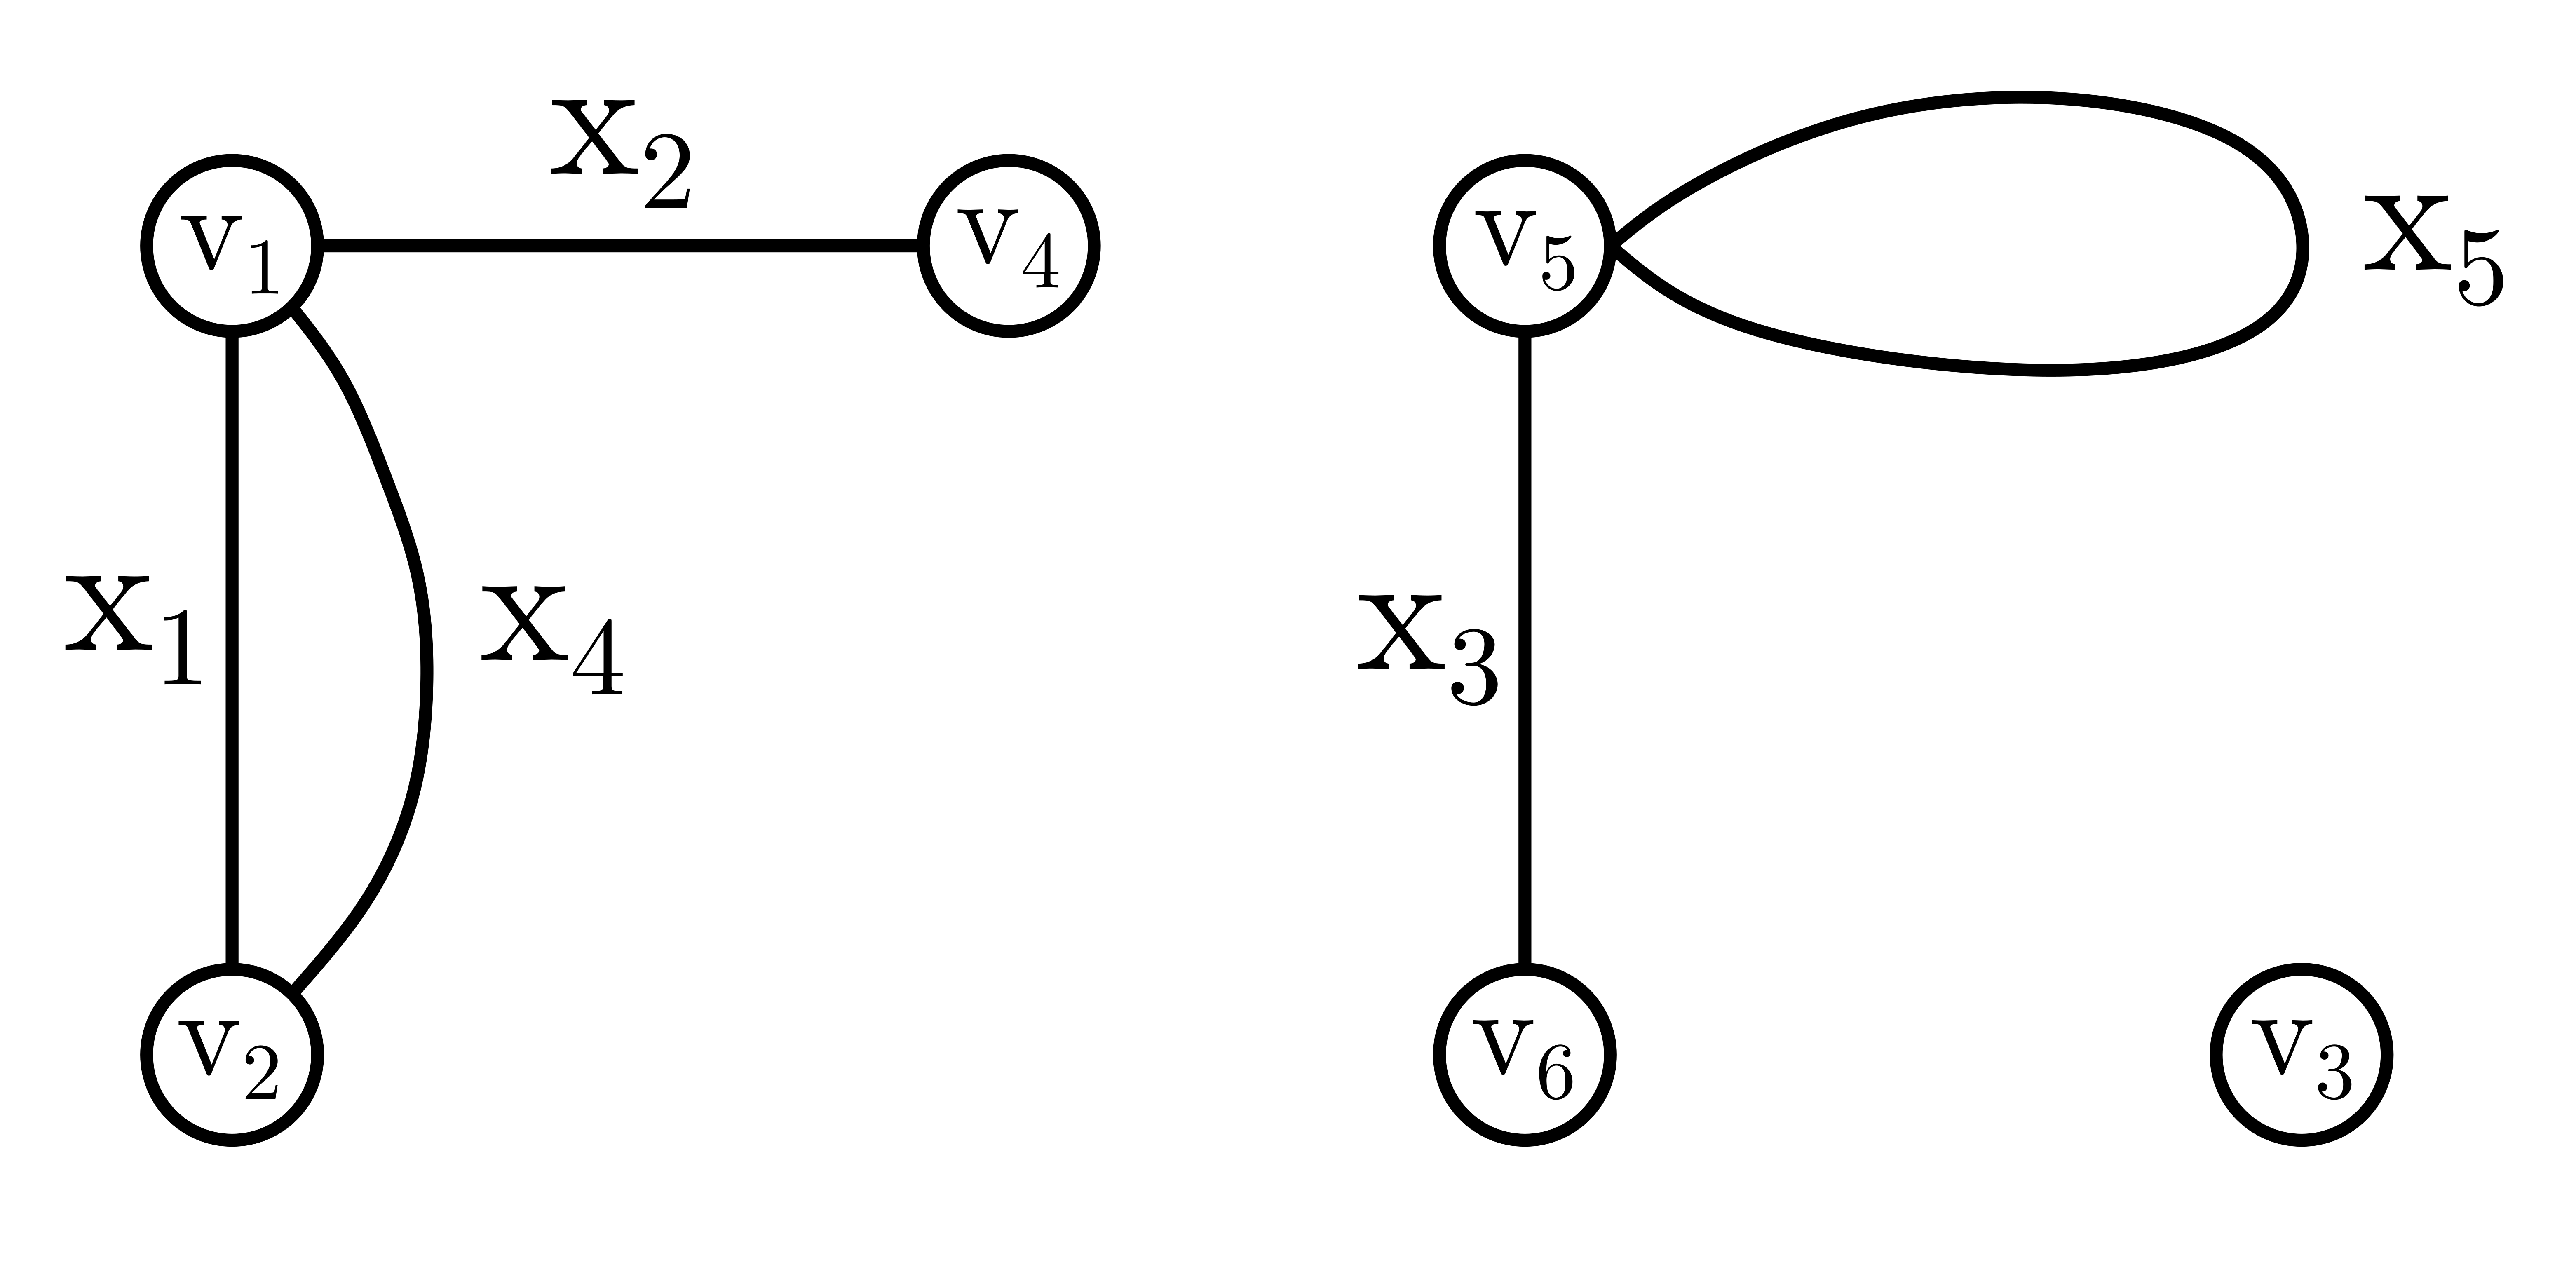
\includegraphics[width=0.8\textwidth]{./images/graph-example.png}
    \end{figure}

    \noindent Проанализировав граф, имеем:
    \[
        d_1 = 3,
        \quad
        d_2 = 2,
        \quad
        d_3 = 0,
        \quad
        d_4 = 1,
        \quad
        d_5 = 3,
        \quad
        d_6 = 1.
    \]
    \[
        \sum_{i = 1}^6 d_i = 10,
        \quad
        m = 5 \; (\text{число ребер}).
    \]
    Таким образом:
    \begin{itemize}
        \item \(v_3\) --- изолированная вершина;
        \item \(v_4\) и \(v_5\) --- висячие вершины.
    \end{itemize}
\end{example*}

\subsection{Изоморфизм графов}

Два графа \(G = (V, X)\) и \(H = (W, Y)\) называют \textbf{изоморфными}, если между их множествами вершин \(V\) и \(W\) существует взаимно однозначное соответствие, сохраняющее смежность. Изоморфизм есть отношение эквивалентности на графах. Из определения следует, что изоморфные графы отличаются лишь обозначением вершин.

\begin{example*}
    Графы \(G\) и \(H\), изображенные на рисунке, изоморфны.
    \begin{figure}[H]
        \centering
        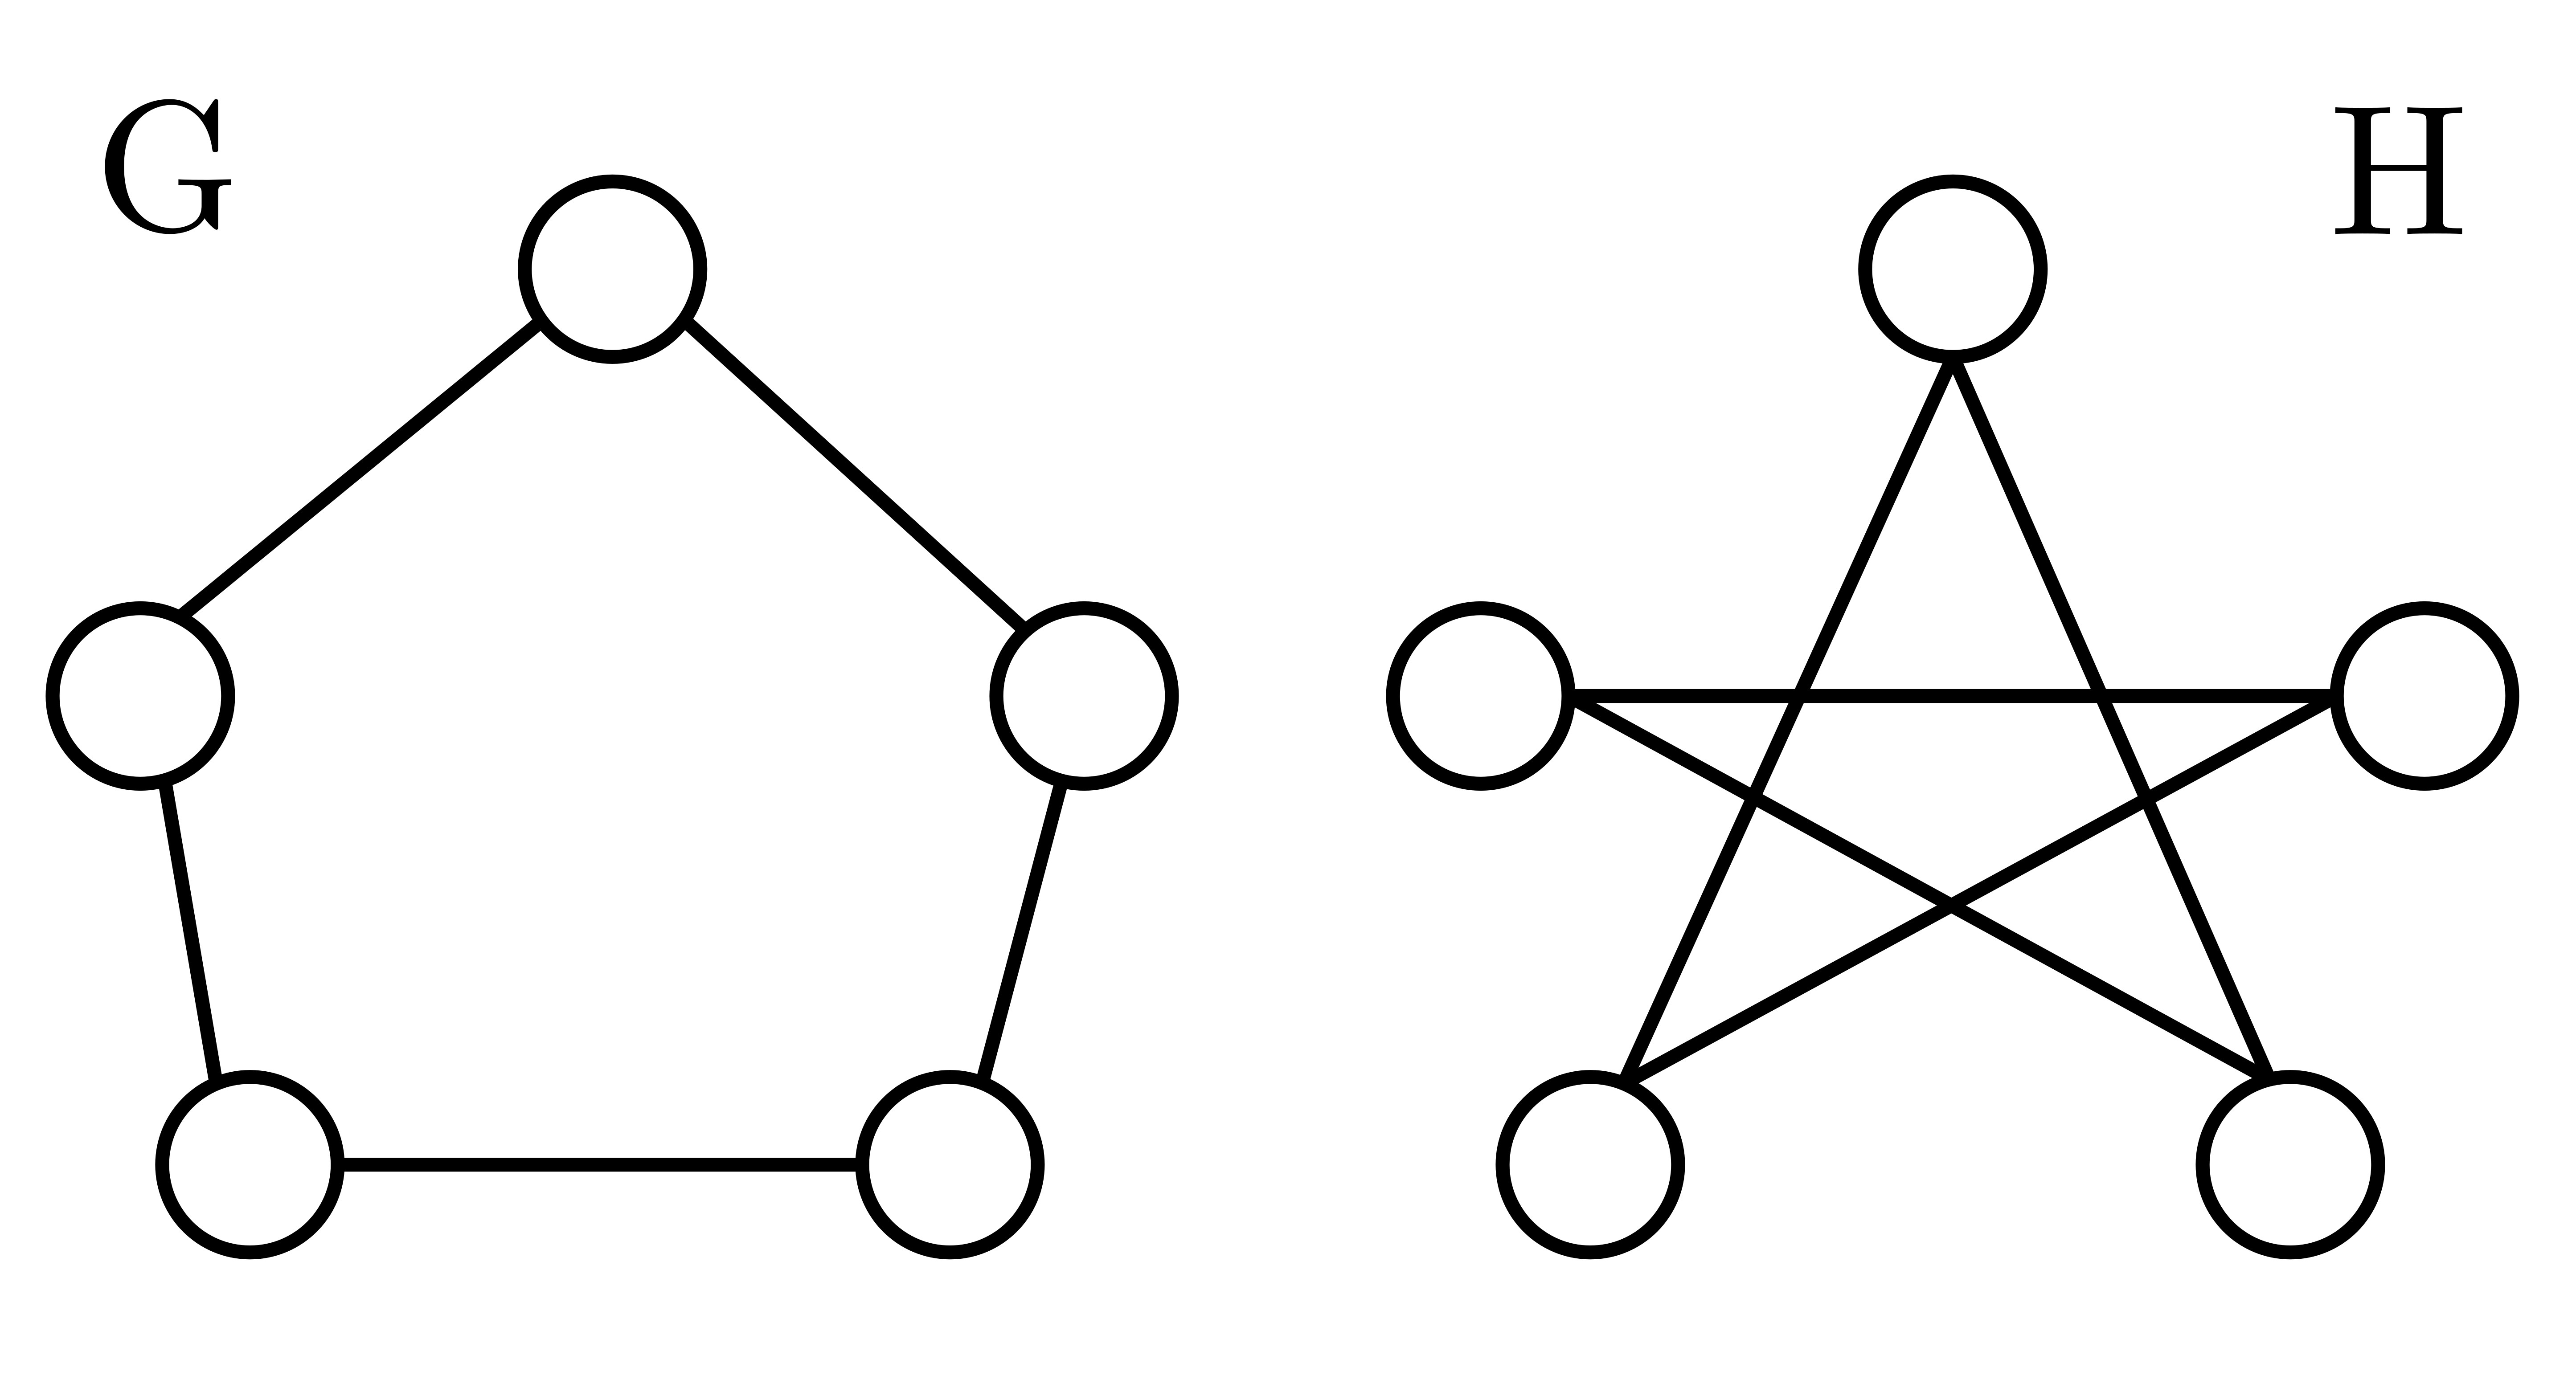
\includegraphics[width=0.7\textwidth]{./images/graph-isomorphism-1.png}
    \end{figure}

    Для того, чтобы доказать их изоморфность, достаточно пометить их вершины в соответствующем порядке:
    \begin{figure}[H]
        \centering
        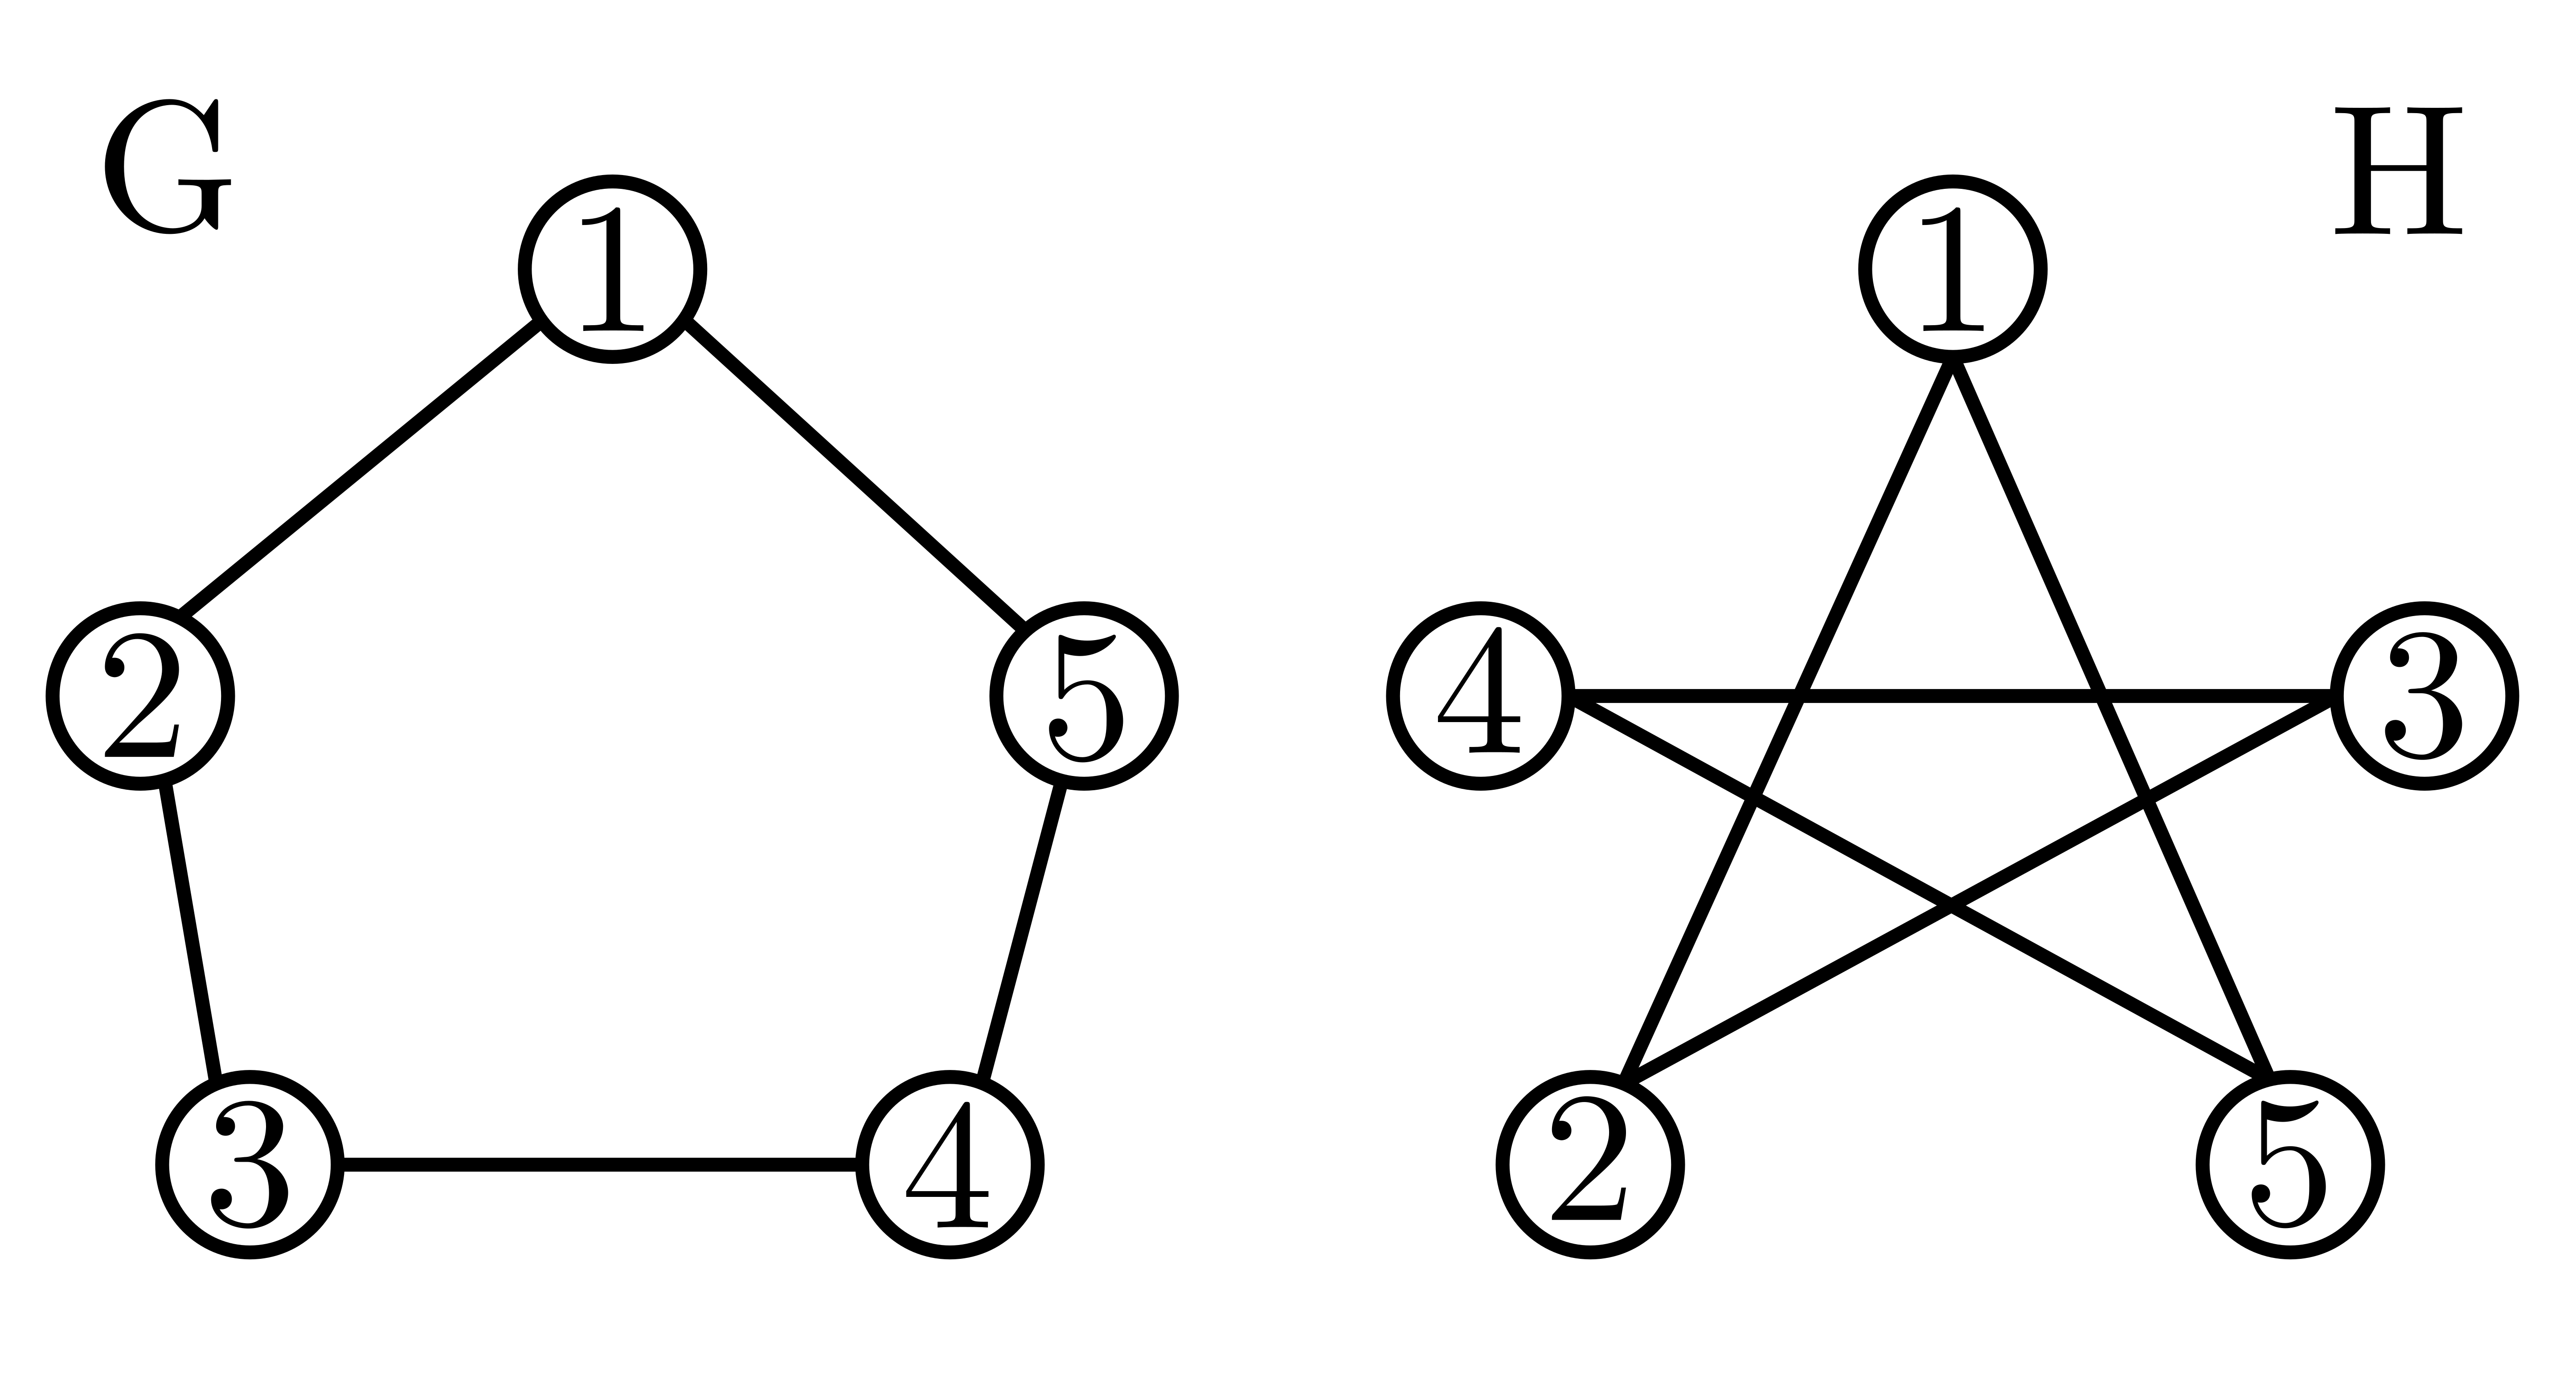
\includegraphics[width=0.7\textwidth]{./images/graph-isomorphism-2.png}
    \end{figure}
\end{example*}

\subsection{Элементы графов}

\textbf{Инвариант} графа \(G\) --- это число, связанное с \(G\), которое принимает одно и то же значение на любом графе, изоморфном \(G\). Числа \(n\) (число вершин графа) и \(m\) (число ребер) являются инвариантами графа.

\textbf{Полный набор инвариантов} определяет граф с точностью до изоморфизма. Например, числа \(n\) и \(m\) образуют полный набор инвариантов для всех графов с \(n < 4\).

\textbf{Подграфом} \(G_0 = (V_0, X_0)\) графа \(G = (V, X)\) называется граф, у которого все вершины и ребра (дуги) принадлежат \(G: V_0 \subset V, X_0 \subset X\), каждое из ребер \(x_i\) инцидентно только вершинам из \(V\). Если \(G_0\) --- подграф, то \(G\) --- \textbf{надграф} графа \(G_0\).

\textbf{Остовной подграф} --- это подграф \(G\), содержащий все его вершины.

\begin{example*}
    На рисунке представлены графы \(G\), \(G_1\) и \(G_2\), причем \(G_1\) и \(G_2\) являются подграфами \(G\).
    \begin{figure}[H]
        \centering
        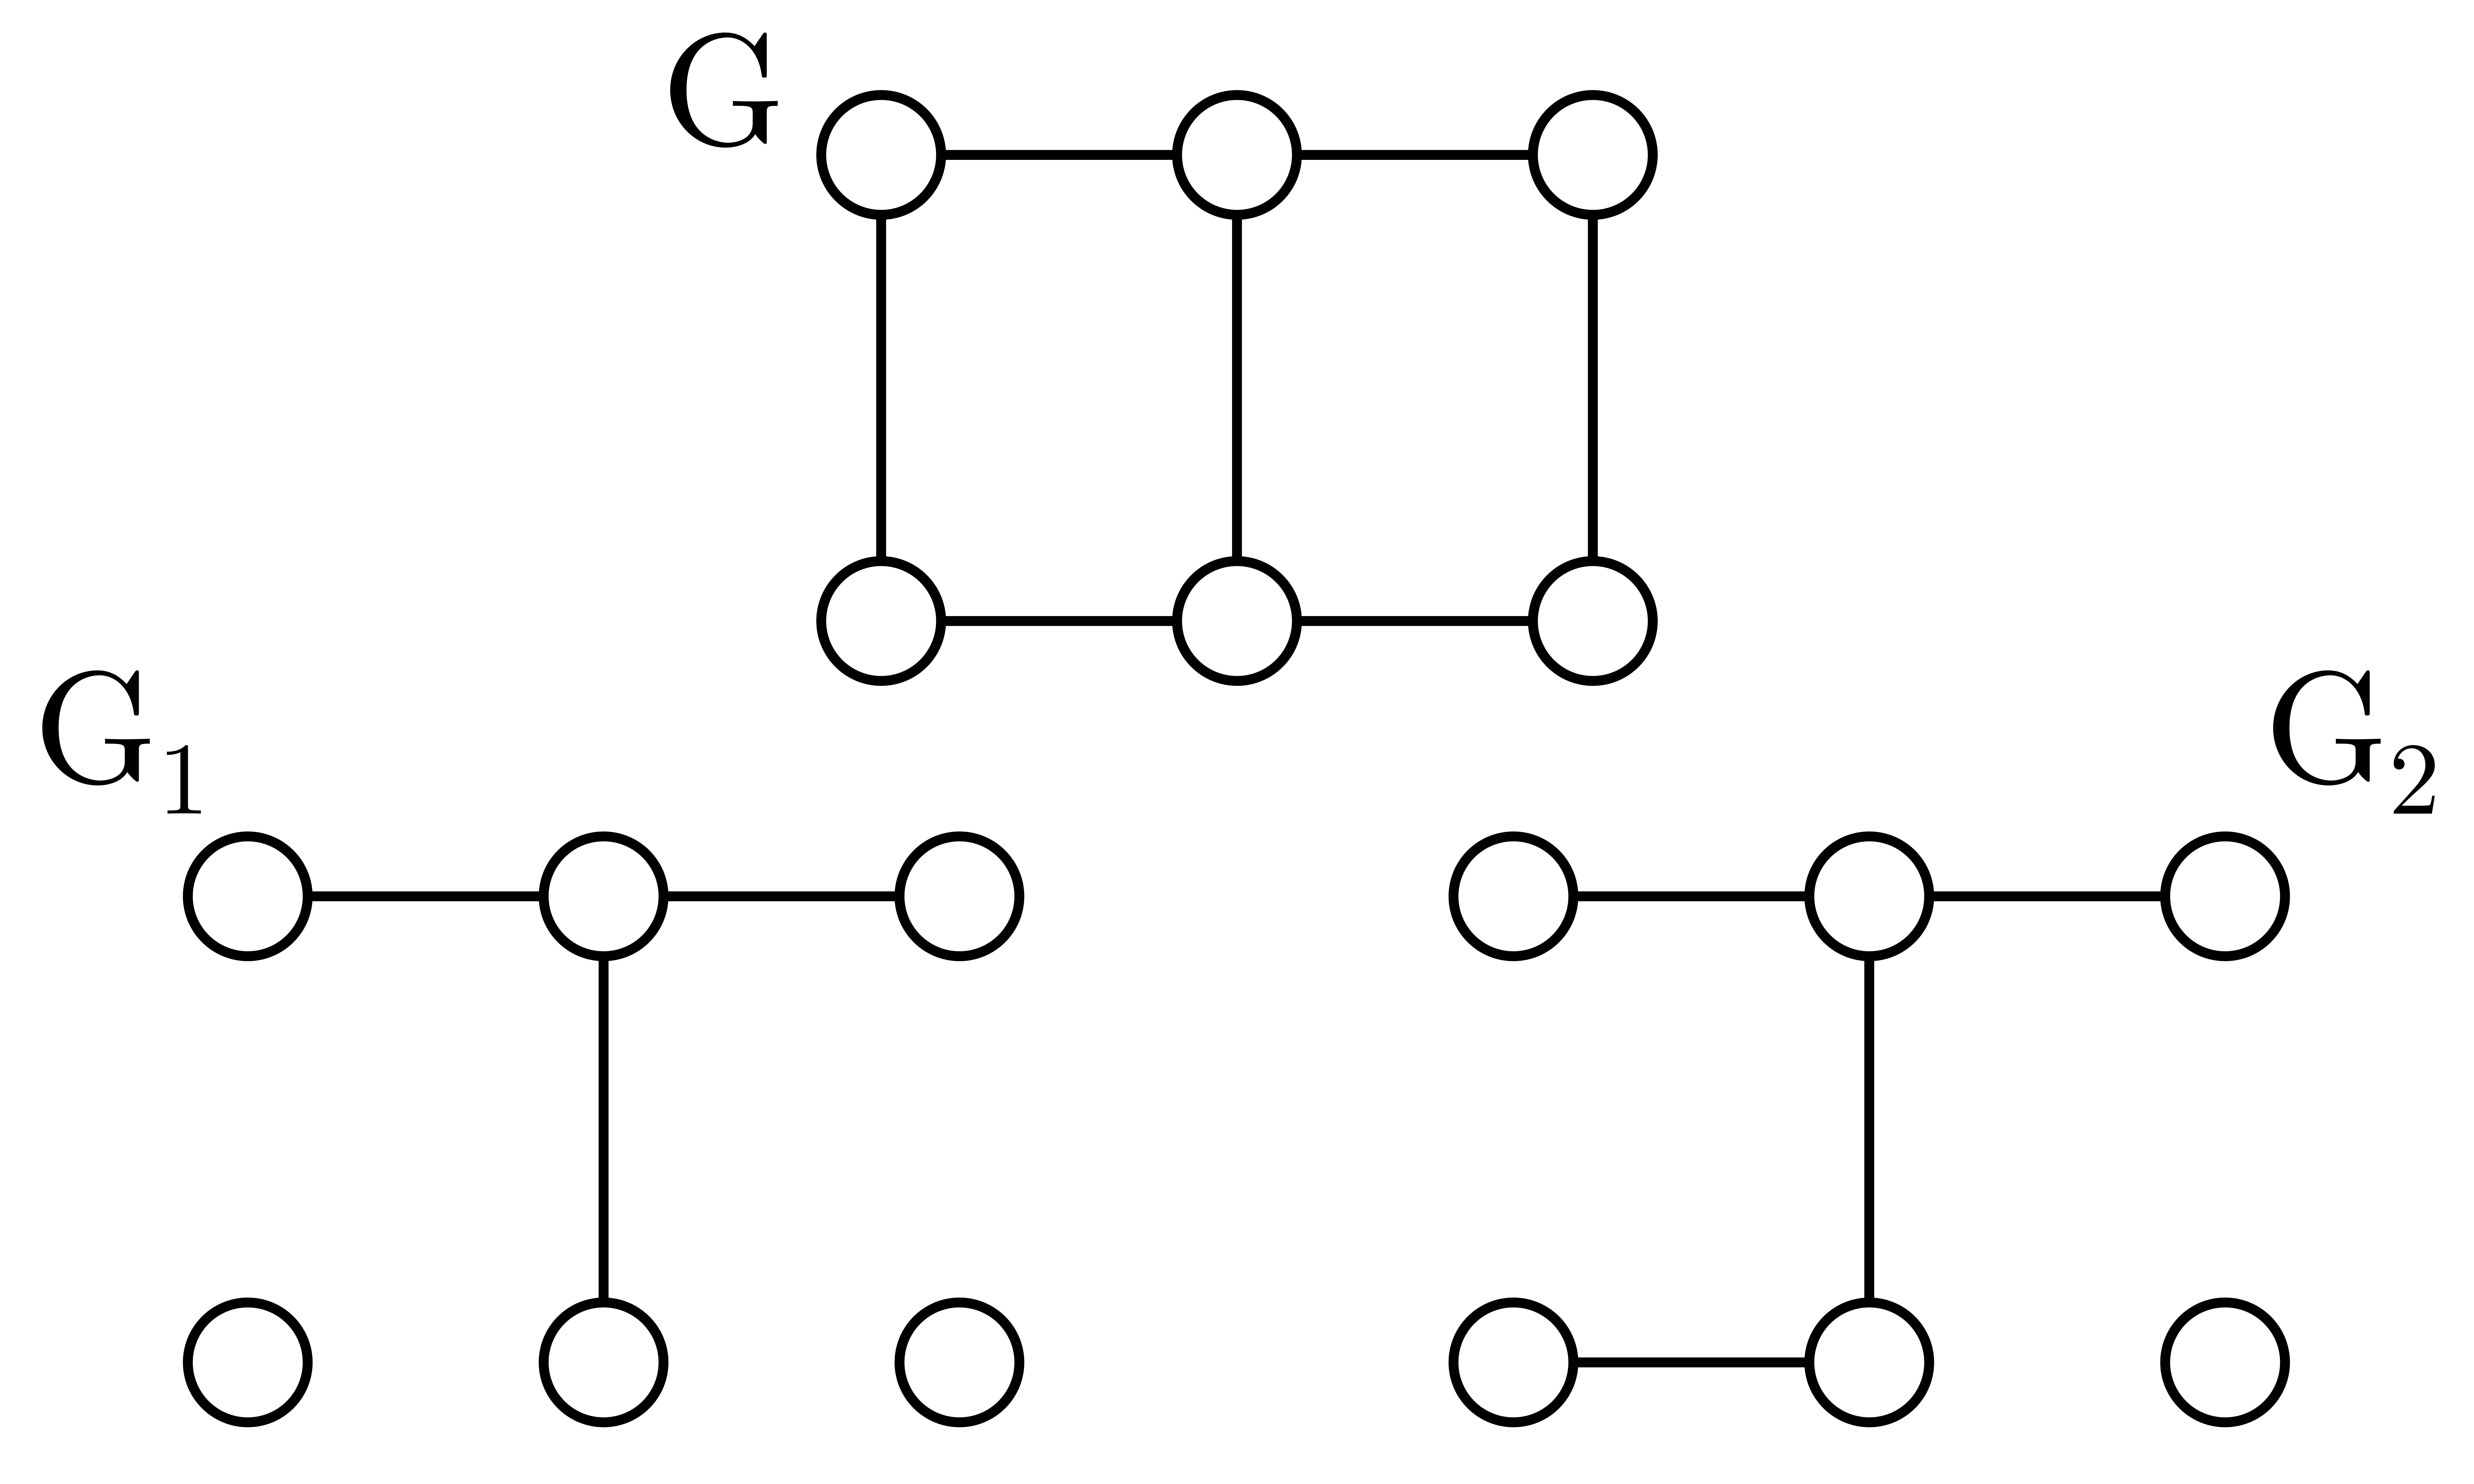
\includegraphics[width=0.8\textwidth]{./images/subgraph-example.png}
    \end{figure}
\end{example*}

\subsection{Маршруты}

Последовательность ребер \((v_0, v_1), (v_1, v_2), \ldots, (v_{i - 1}, v_i), \ldots, (v_{r - 1}, v_r)\) называется \textbf{маршрутом}, соединяющим вершины \(v_0\) и \(v_r\). Указанный маршрут можно обозначать также последовательностью вершин \(v_0, v_1, \ldots, v_r\).

Маршрут \textbf{замкнут}, если \(v_0 = v_r\), и \textbf{открыт} в противоположном случае. Маршрут называется \textbf{цепью}, если все его ребра различны, и \textbf{простой цепью}, если его вершины различны.

Замкнутая (простая) цепь называется (простым) \textbf{циклом}. В случае орграфа вместо слова <<цепь>> используются <<путь>>, а слово <<цикл>> заменяют на слово \textbf{<<контур>>}.

\begin{example*}
    Рассмотрим следующий граф:

    \begin{figure}[H]
        \centering
        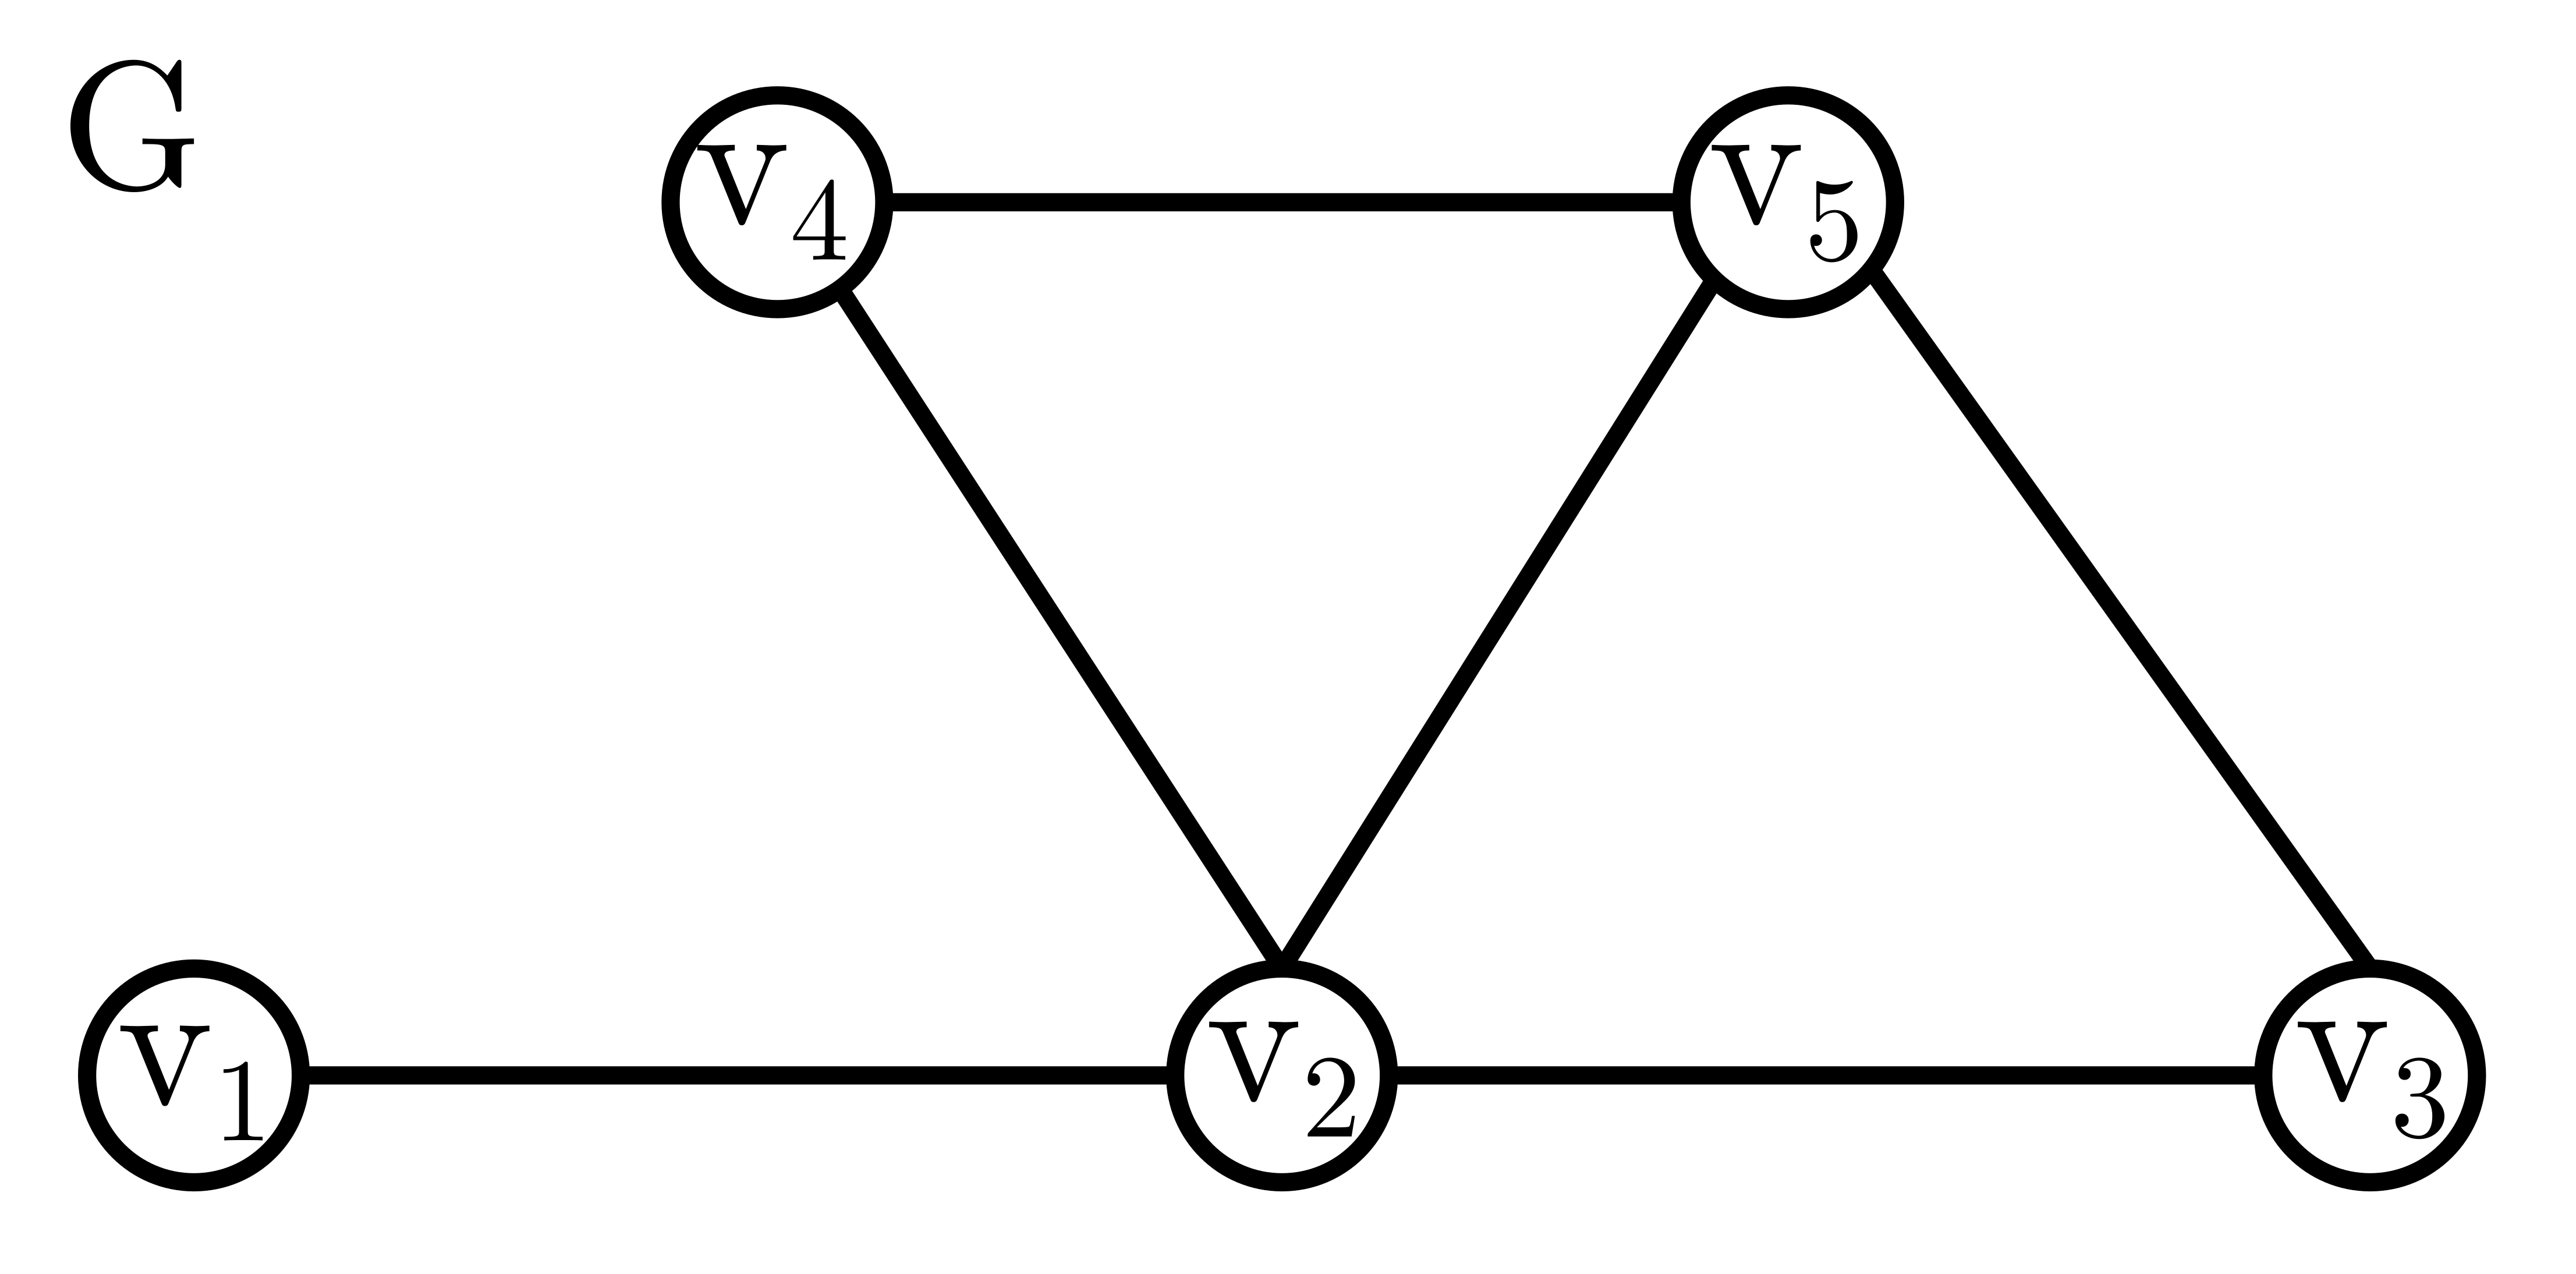
\includegraphics[width=0.65\textwidth]{./images/route-example.png}
    \end{figure}

    \noindent В данном случае
    \begin{itemize}
        \item \(v_1\)-\(v_2\)-\(v_5\)-\(v_2\)-\(v_3\) --- маршрут, который не является цепью;
        \item \(v_1\)-\(v_2\)-\(v_5\)-\(v_4\)-\(v_2\)-\(v_3\) --- цепь, которая не является простой;
        \item \(v_1\)-\(v_2\)-\(v_5\)-\(v_4\) --- простая цепь;
        \item \(v_2\)-\(v_4\)-\(v_5\)-\(v_2\) --- простой цикл.
    \end{itemize}
\end{example*}

\subsection{Связность}

Граф называется \textbf{связным}, если любая пара его вершин соединена маршрутом. \textbf{Компонентой связности} называется максимальный связный подграф графа \(G\). Изолированную вершину также следует рассматривать как компоненту связности.

Несвязный граф имеет, по крайней мере, две компоненты связности. Если граф \(G\) связен, то он имеет только одну компоненту, которая является подграфом \(G\).

Число компонент связности графа \(G\) обозначается \(k(G)\). Граф \(G\) связен тогда и только тогда, когда \(k(G) = 1\).

Граф называется \textbf{вполне несвязным}, если он состоит только из изолированных вершин. Граф называется \(\pmb{K}\)\textbf{-связным}, если удаление не менее \(K\) вершин (ребер) приводит к потере свойства связности. Связный граф с наименьшим числом ребер (или связный граф без циклов) называется \textbf{деревом}.

\begin{example*}
    Рассмотрим следующий граф:
    \begin{figure}[H]
        \centering
        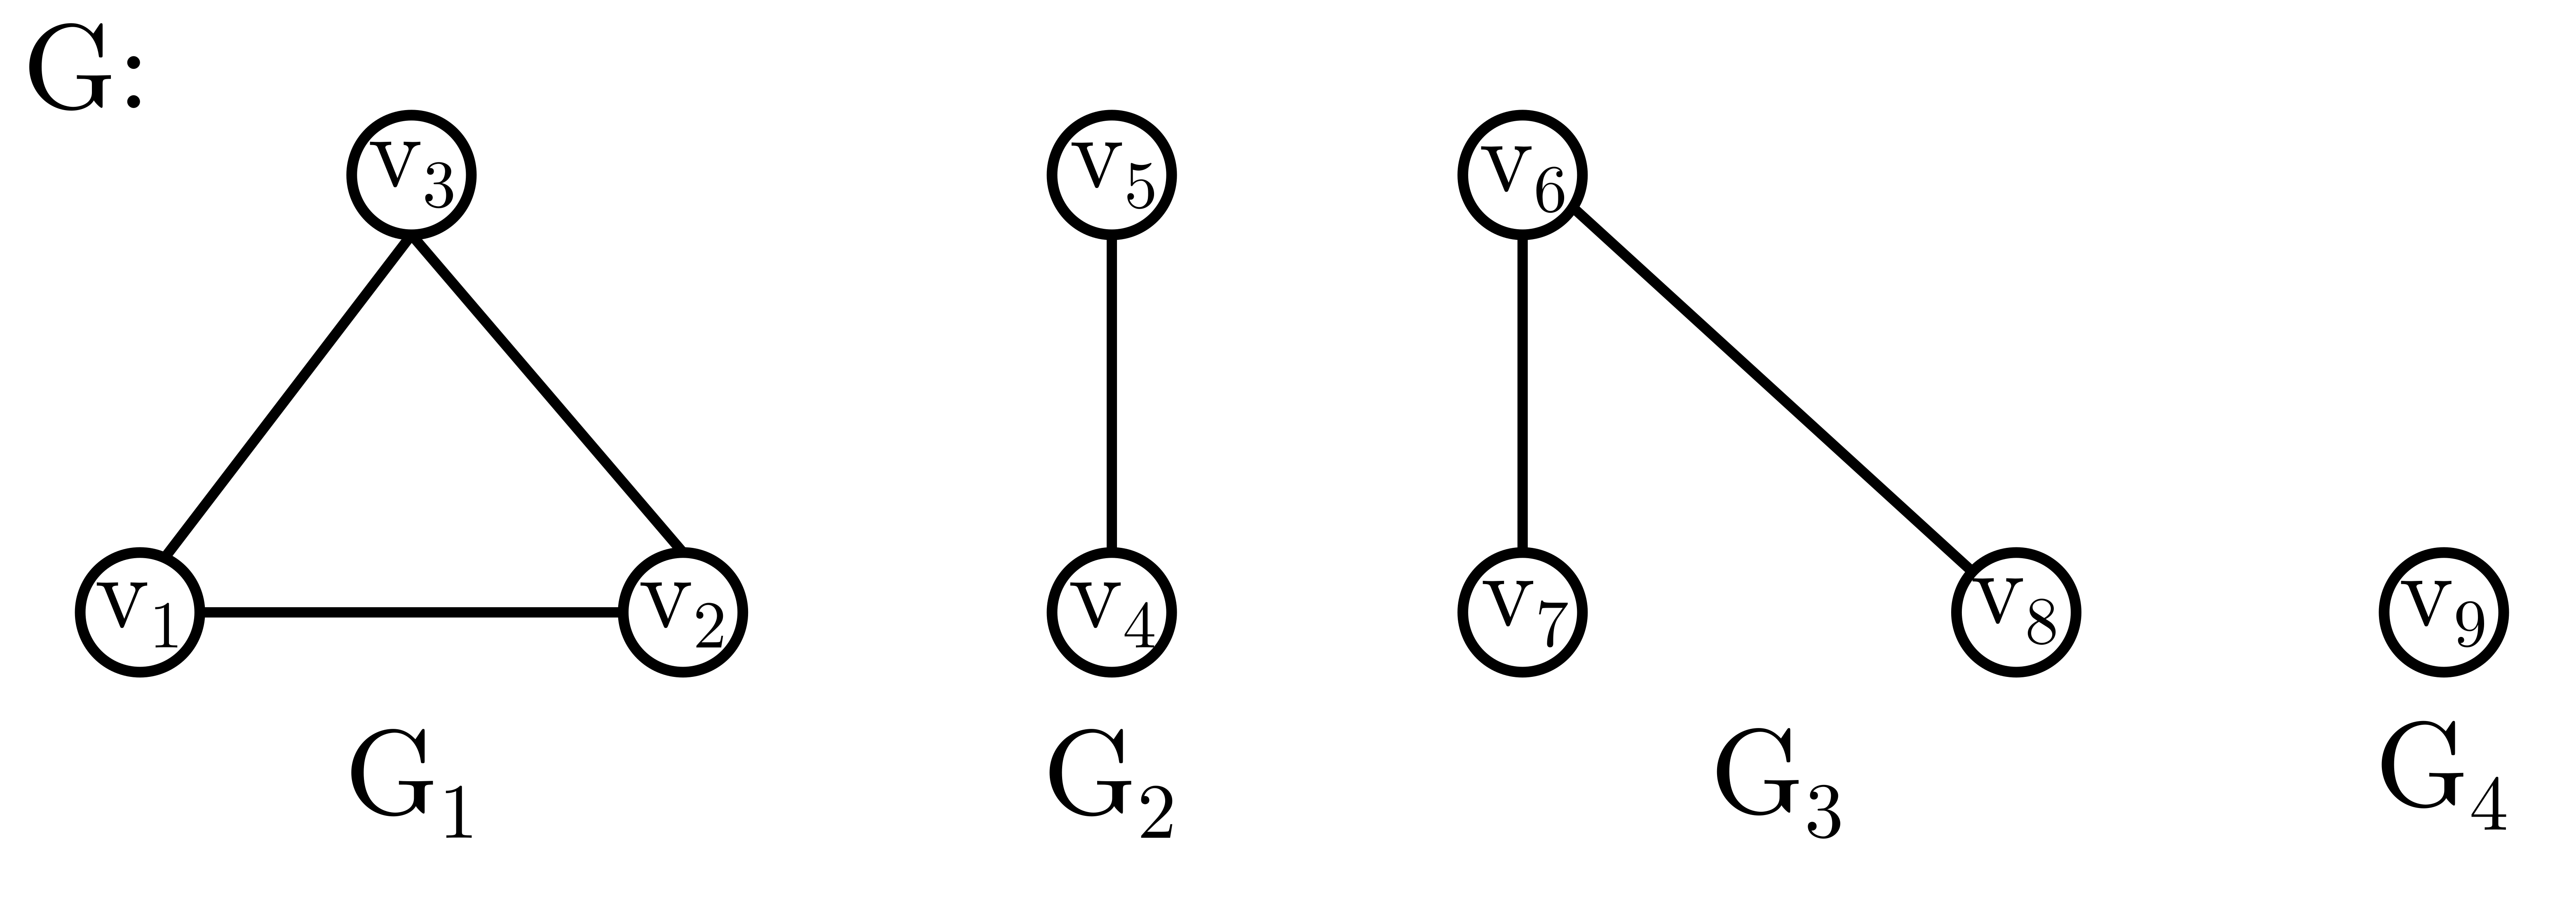
\includegraphics[width=0.9\textwidth]{./images/graph-connectivity.png}
    \end{figure}

    \noindent Граф \(G\) не связен и имеет \(4\) компоненты: \(G_1\), \(G_2\), \(G_3\) и \(G_4\).
\end{example*}

\subsection{Длина маршрута}

\textbf{Длина маршрута} (цепи, простой цепи) равна количеству ребер в порядке их прохождения (каждое ребро считается столько раз, сколько оно встречается в данном маршруте).

Длина кратчайшей простой цепи, соединяющей вершины \(v_i\) и \(v_j\) в графе \(G\), называется \textbf{расстоянием} между \(v_i\) и \(v_j\) и обозначается \(d(v_i, v_j)\). Если вершины \(v_i\) и \(v_j\) не соединены, то полагают \(d(v_i, v_j) = \infty\).

В связном неориентированном графе расстояние удовлетворяет аксиомам метрики. Так, для любых трех вершин \(u\), \(v\) и \(w\)
\begin{enumerate}
    \item \(d(u, v) \geq 0\) и \(d(u, v) = 0 \iff u = v\);
    \item \(d(u, v) = d(v, u)\);
    \item \(d(u, v) + d(v, w) \geq d(u, w)\).
\end{enumerate}

\subsection{Метрические характеристики графа}

\textbf{Эксцентриситетом} вершины \(v\) в связном графе \(G\) называется максимальное расстояние от вершины \(v\) до других вершин графа \(G\):
\[
    e(v) = \max\limits_{u \in V} d(u, v).
\]

\textbf{Радиусом} графа называется наименьший из эксцентриситетов вершин и обозначается \(R(G)\). \textbf{Диаметром} графа называется наибольший из эксцентриситетов вершин и обозначается \(D(G)\).

Вершина \(v\) называется \textbf{центральной вершиной} графа \(G\), если выполняется равенство \(e(v) = R(G)\). \textbf{Центр графа} --- это множество всех центральных вершин:
\[
    C(G) = \{v \in V \mid e(v) = R(G)\}.
\]

\begin{theorem*}
    Каждое дерево имеет центр, состоящий или из одной вершины, или из двух смежных вершин.
\end{theorem*}

\begin{example*}
    Вершины и их эксцентриситеты:
    \begin{figure}[H]
        \centering
        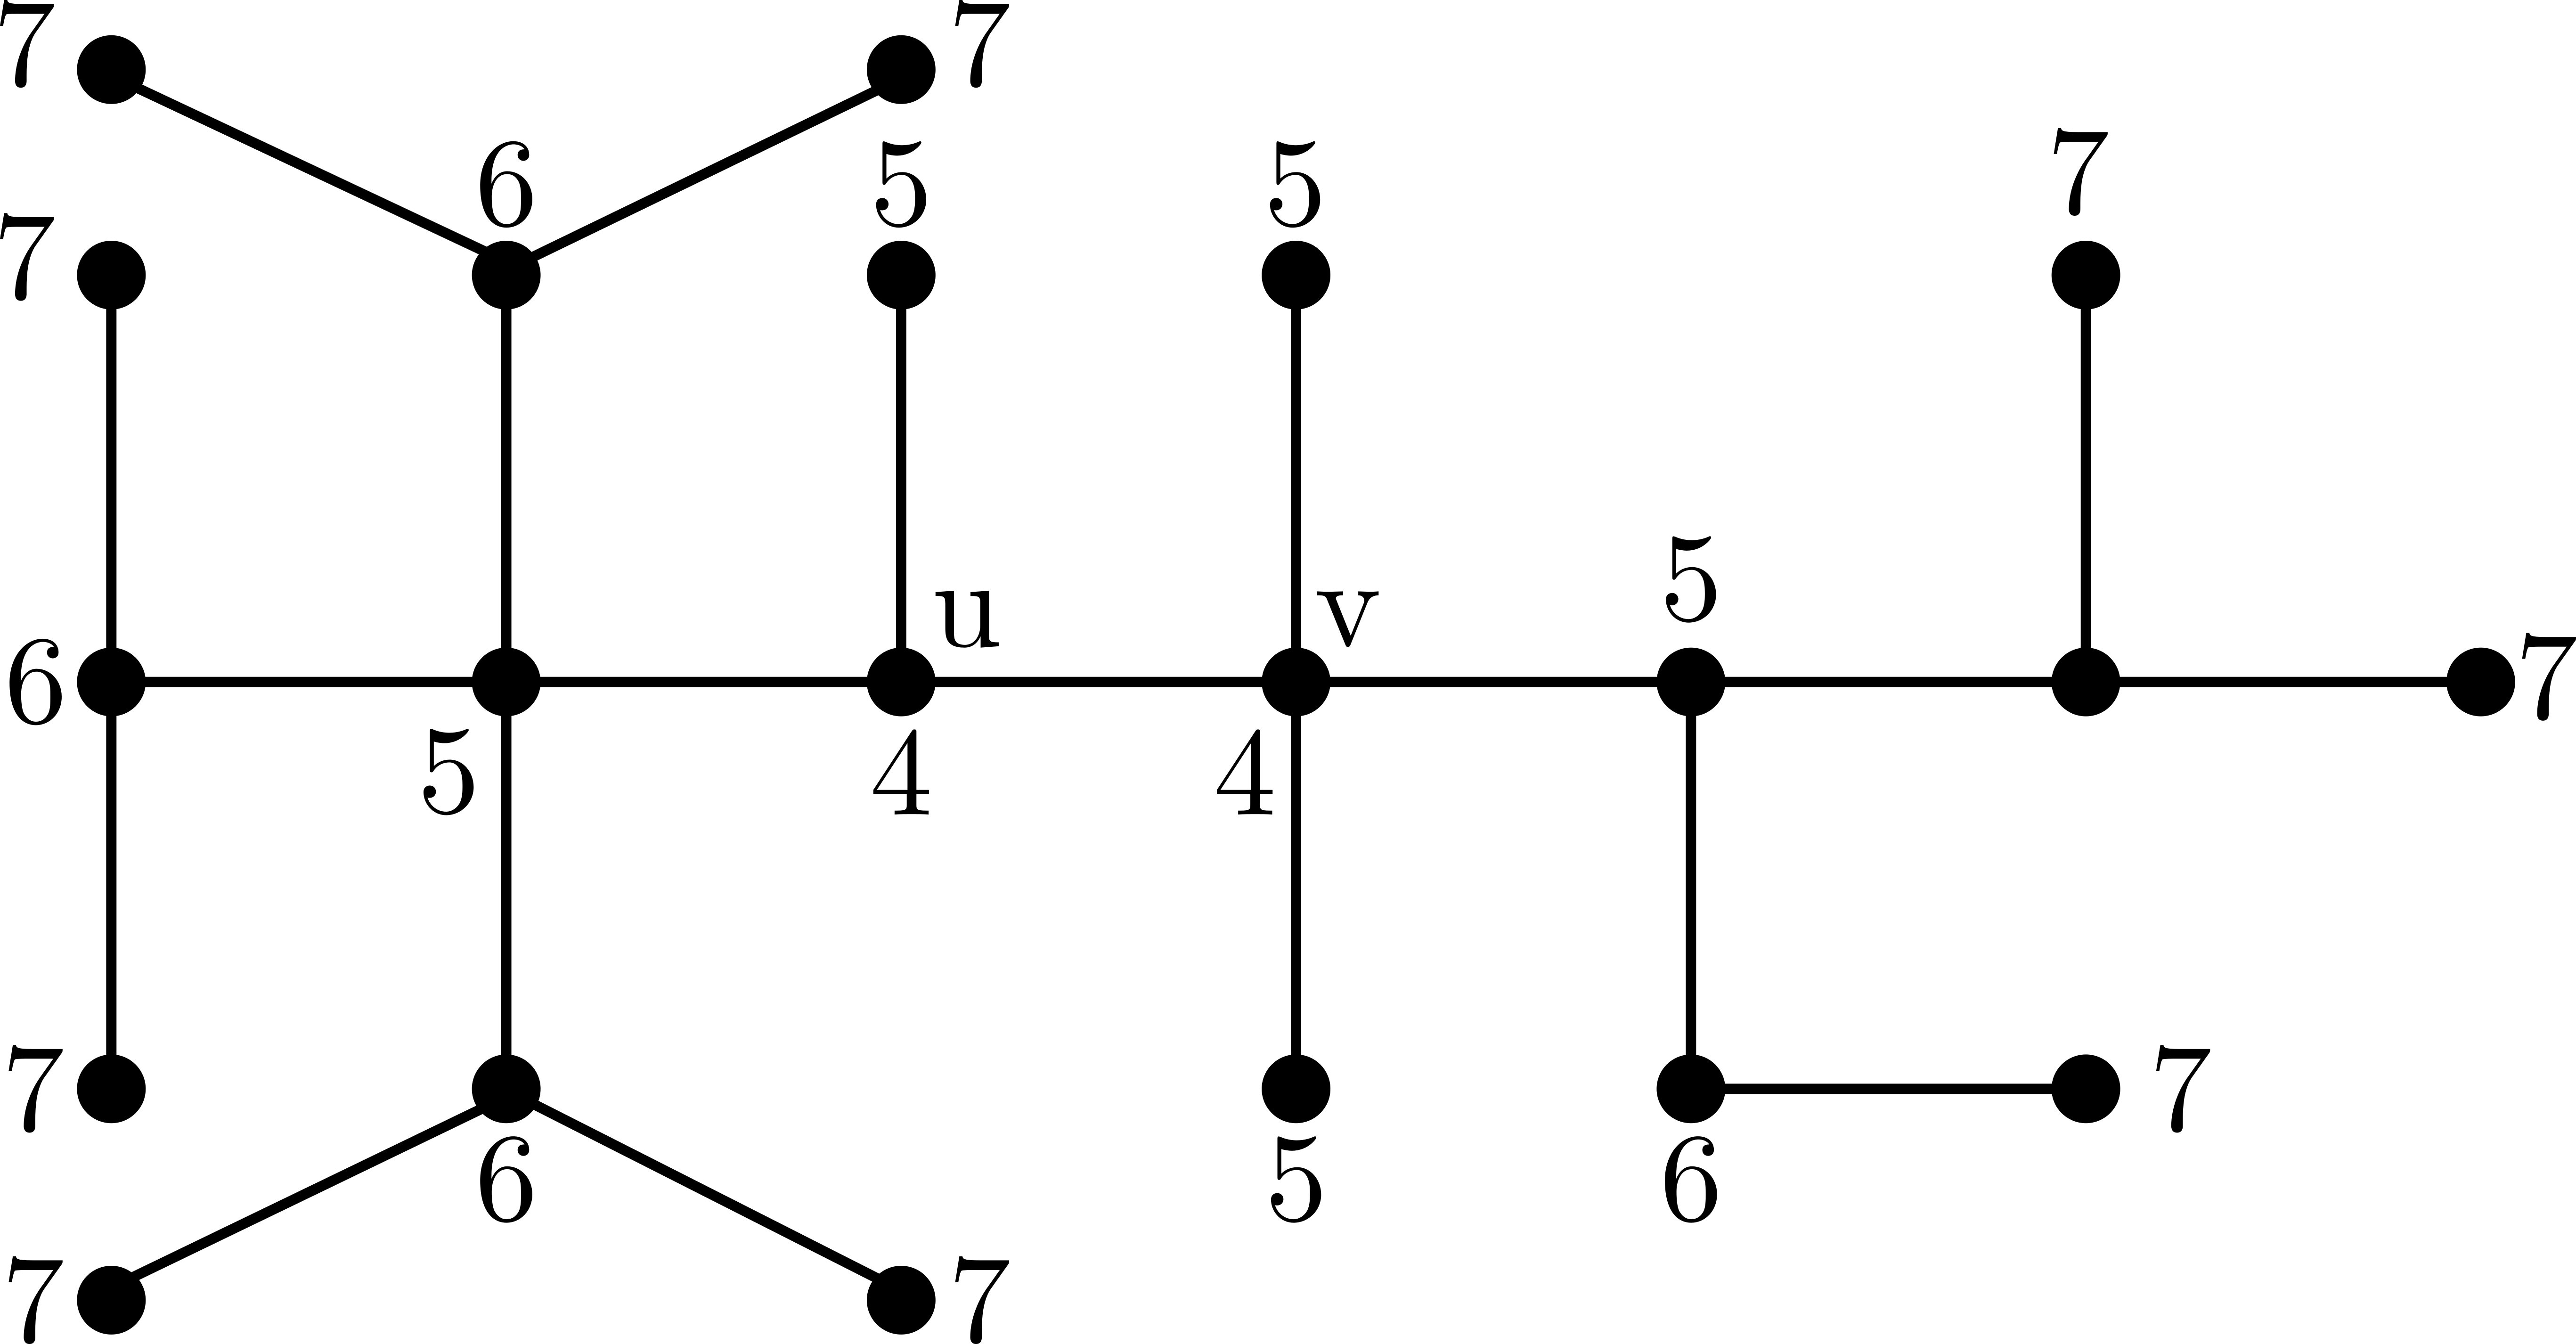
\includegraphics[width=0.8\textwidth]{./images/eccentricities.png}
    \end{figure}

    В данном случае
    \[
        D(G) = 7,
        \qquad
        R(G) = 4,
        \qquad
        C(G) = \{u, v\}.
    \]
\end{example*}

\subsection{Однородные графы}

Если все вершины имеют одинаковую степень \(r\), то такой граф \(G\) называется \textbf{регулярным} (или однородным) степени \(r\). В этом случае говорят о степени графа и пишут \(\deg G = r\).

Регулярные графы степени \(3\) называются \textbf{кубическими}. Каждый кубический граф имеет четное число вершин.

\begin{example*}
    Кубические графы с шестью вершинами:
    \begin{figure}[H]
        \centering
        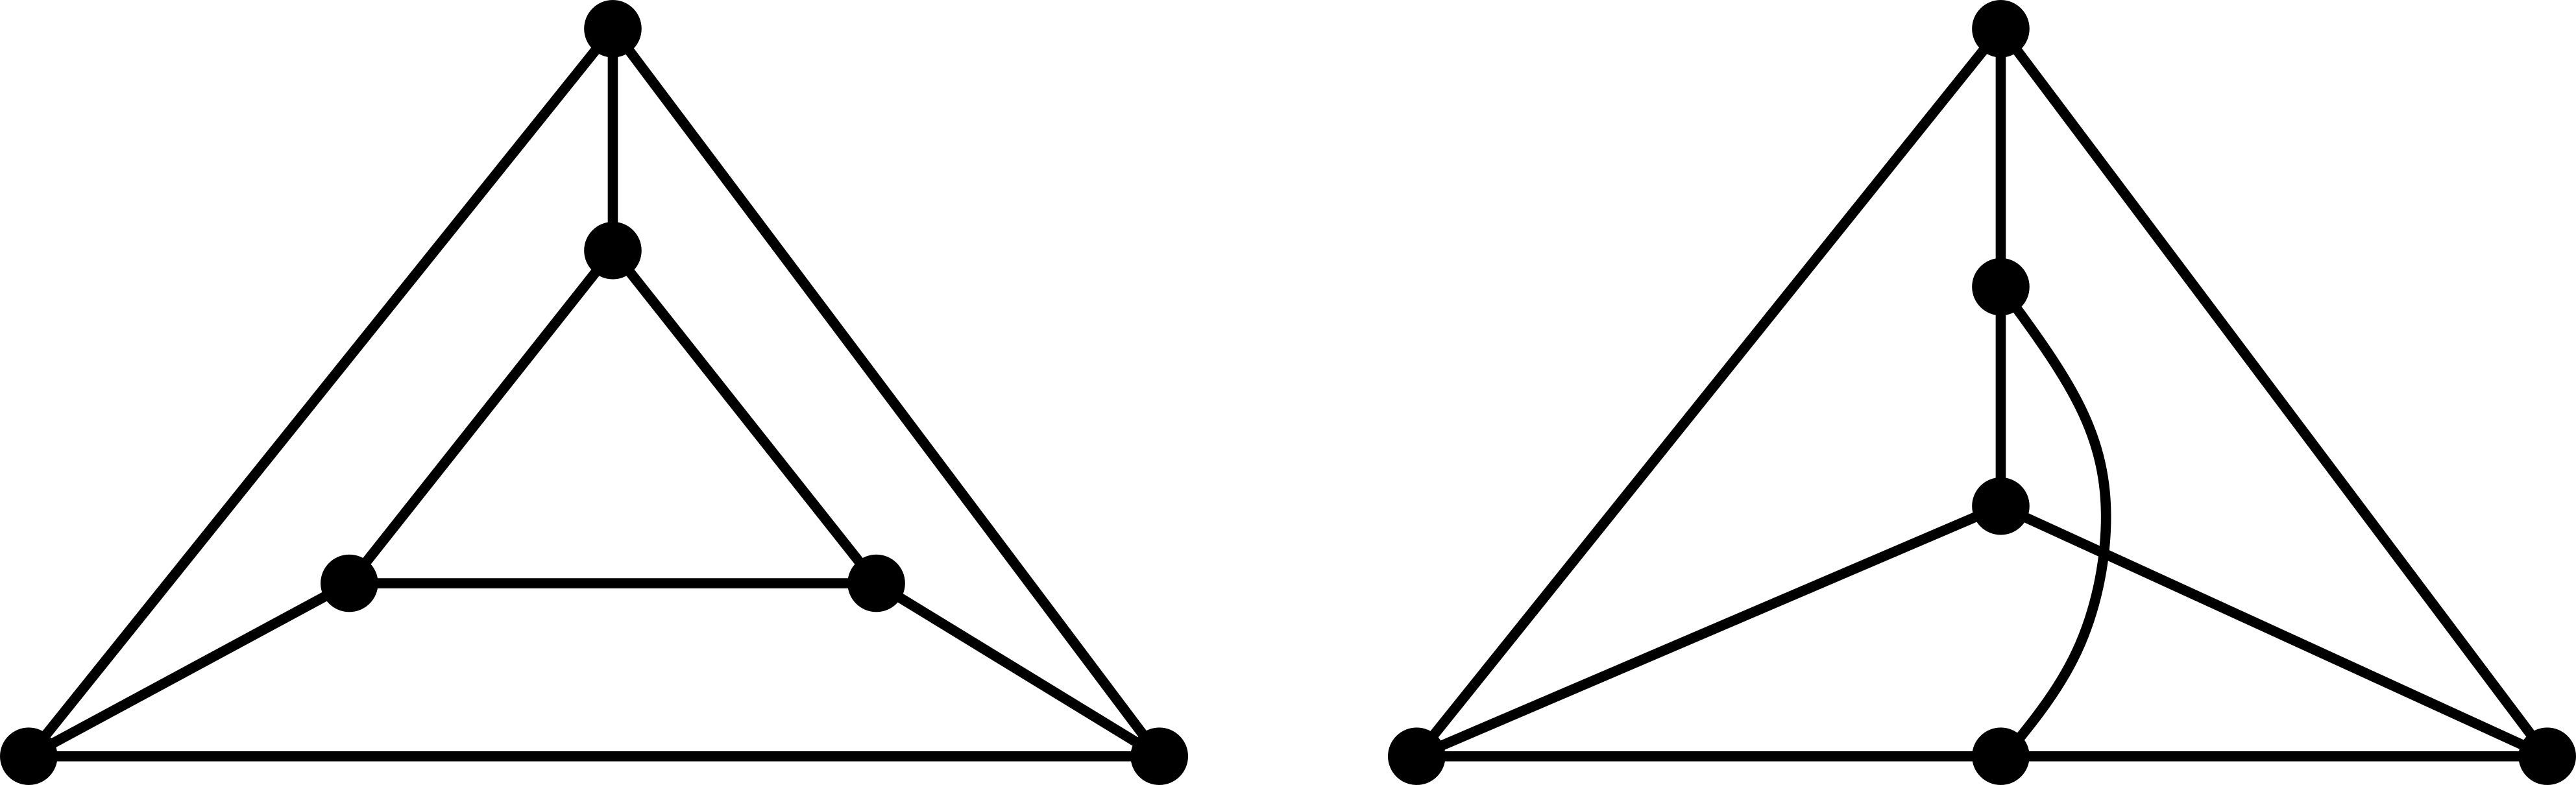
\includegraphics[width=0.8\textwidth]{./images/homogeneous-graphs.png}
    \end{figure}
\end{example*}

\subsection{Полные графы}

Граф, в котором любые две вершины смежны, называется \textbf{полным}. Полный граф с \(n\) вершинами обозначается \(K_n\). Он имеем максимальное число ребер равное
\[
    m = C_n^2 = \frac{n!}{2! (n - 2)!} = \frac{n (n - 1)}{2}.
\]
и является регулярным степени \(n - 1\). Полный подграф некоторого графа называют \textbf{кликой} этого графа.

\begin{example*}
    Полные графы \(K_3\) и \(K_5\):
    \begin{figure}[H]
        \centering
        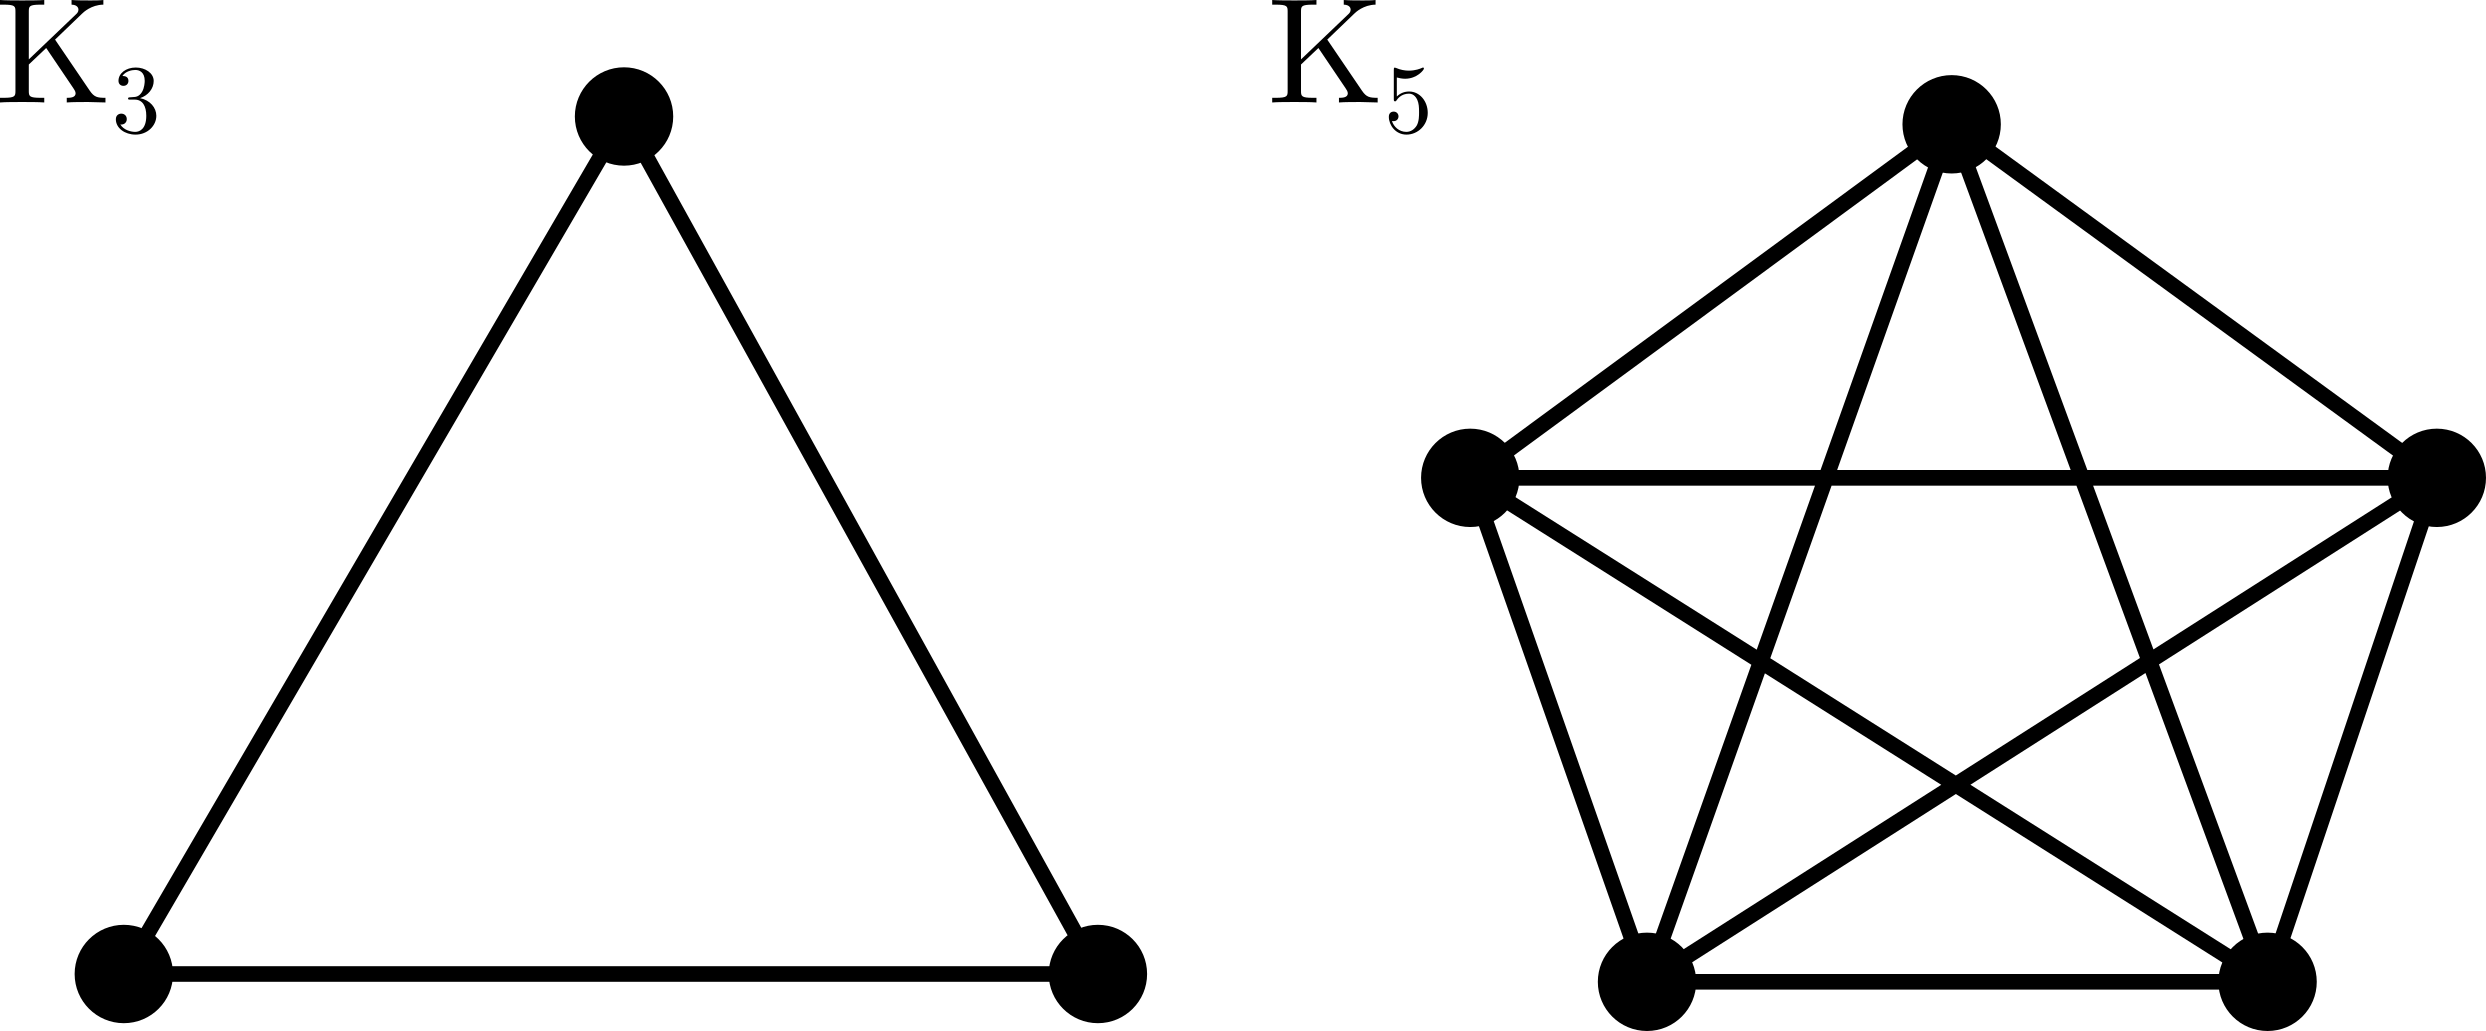
\includegraphics[width=0.7\textwidth]{images/complete-graphs.png}
    \end{figure}
\end{example*}

\subsection{Двудольные графы}

\textbf{Двудольный граф} \(G\) --- это граф, множество вершин \(V\) которого можно разбить на два подмножества \(V_1\) и \(V_2\) таким образом, что каждое ребро графа \(G\) соединяет вершины из разных множеств.

\begin{example*}
    Один и тот же двудольный граф, представленный по разному:
    \begin{figure}[H]
        \centering
        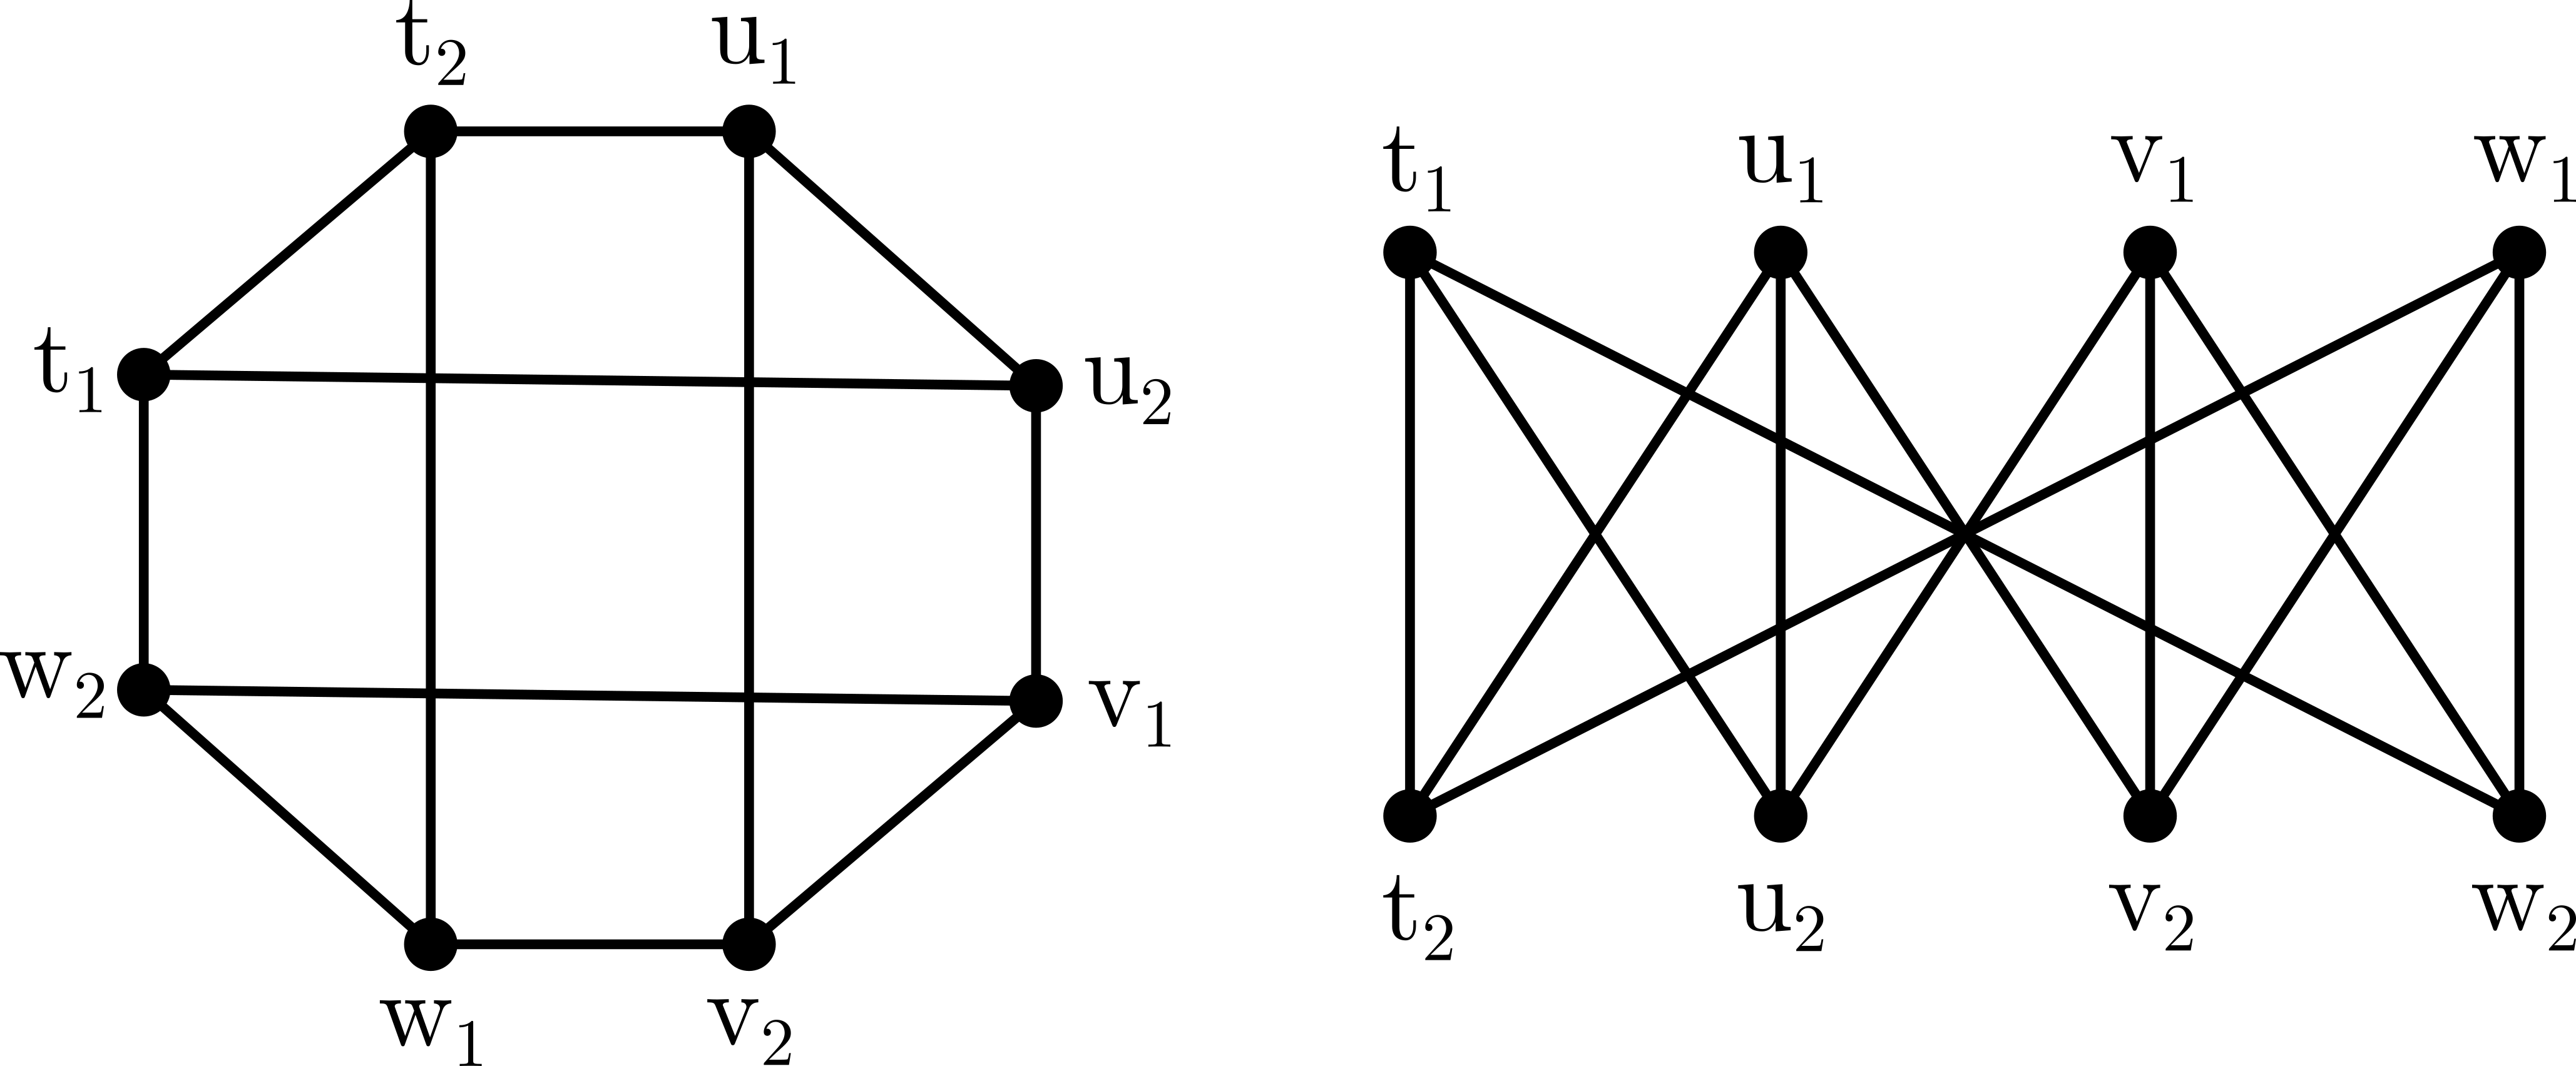
\includegraphics[width=0.9\textwidth]{images/bipartite-graphs.png}
    \end{figure}
\end{example*}

Если граф \(G\) содержит все ребра, соединяющие множества \(V_1\) и \(V_2\), то этот граф называется \textbf{полным двудольным}. Если при этом в множестве \(V_1\) имеется \(m\) вершин, а в \(V_2\) имеется \(n\) вершин, то граф обозначают \(K_{m, n}\). \textbf{Звездой} называется полный двудольный граф \(K_{1, n}\).

\begin{theorem*}[Кенига]
    Для двудольности графа необходимо и достаточно, чтобы он не содержал циклов нечетной длины.
    \begin{consequence*}
        Граф является двудольным тогда и только тогда, когда он не имеет простых циклов нечетной длины.
    \end{consequence*}
\end{theorem*}

\subsection{Самодополнительные графы}

\textbf{Дополнение} \(\bar{G}\) графа \(G\) имеет в качестве множества вершин множество вершин графа \(G\). При этом две вершины \(\bar{G}\) смежны тогда и только тогда, когда они не смежны в \(G\). Графы \(\bar{K}_n\) являются вполне несвязными (или регулярными степени \(0\)).

\begin{example*}
    Граф \(G\) и его дополнение \(\bar{G}\):
    \begin{figure}[H]
        \centering
        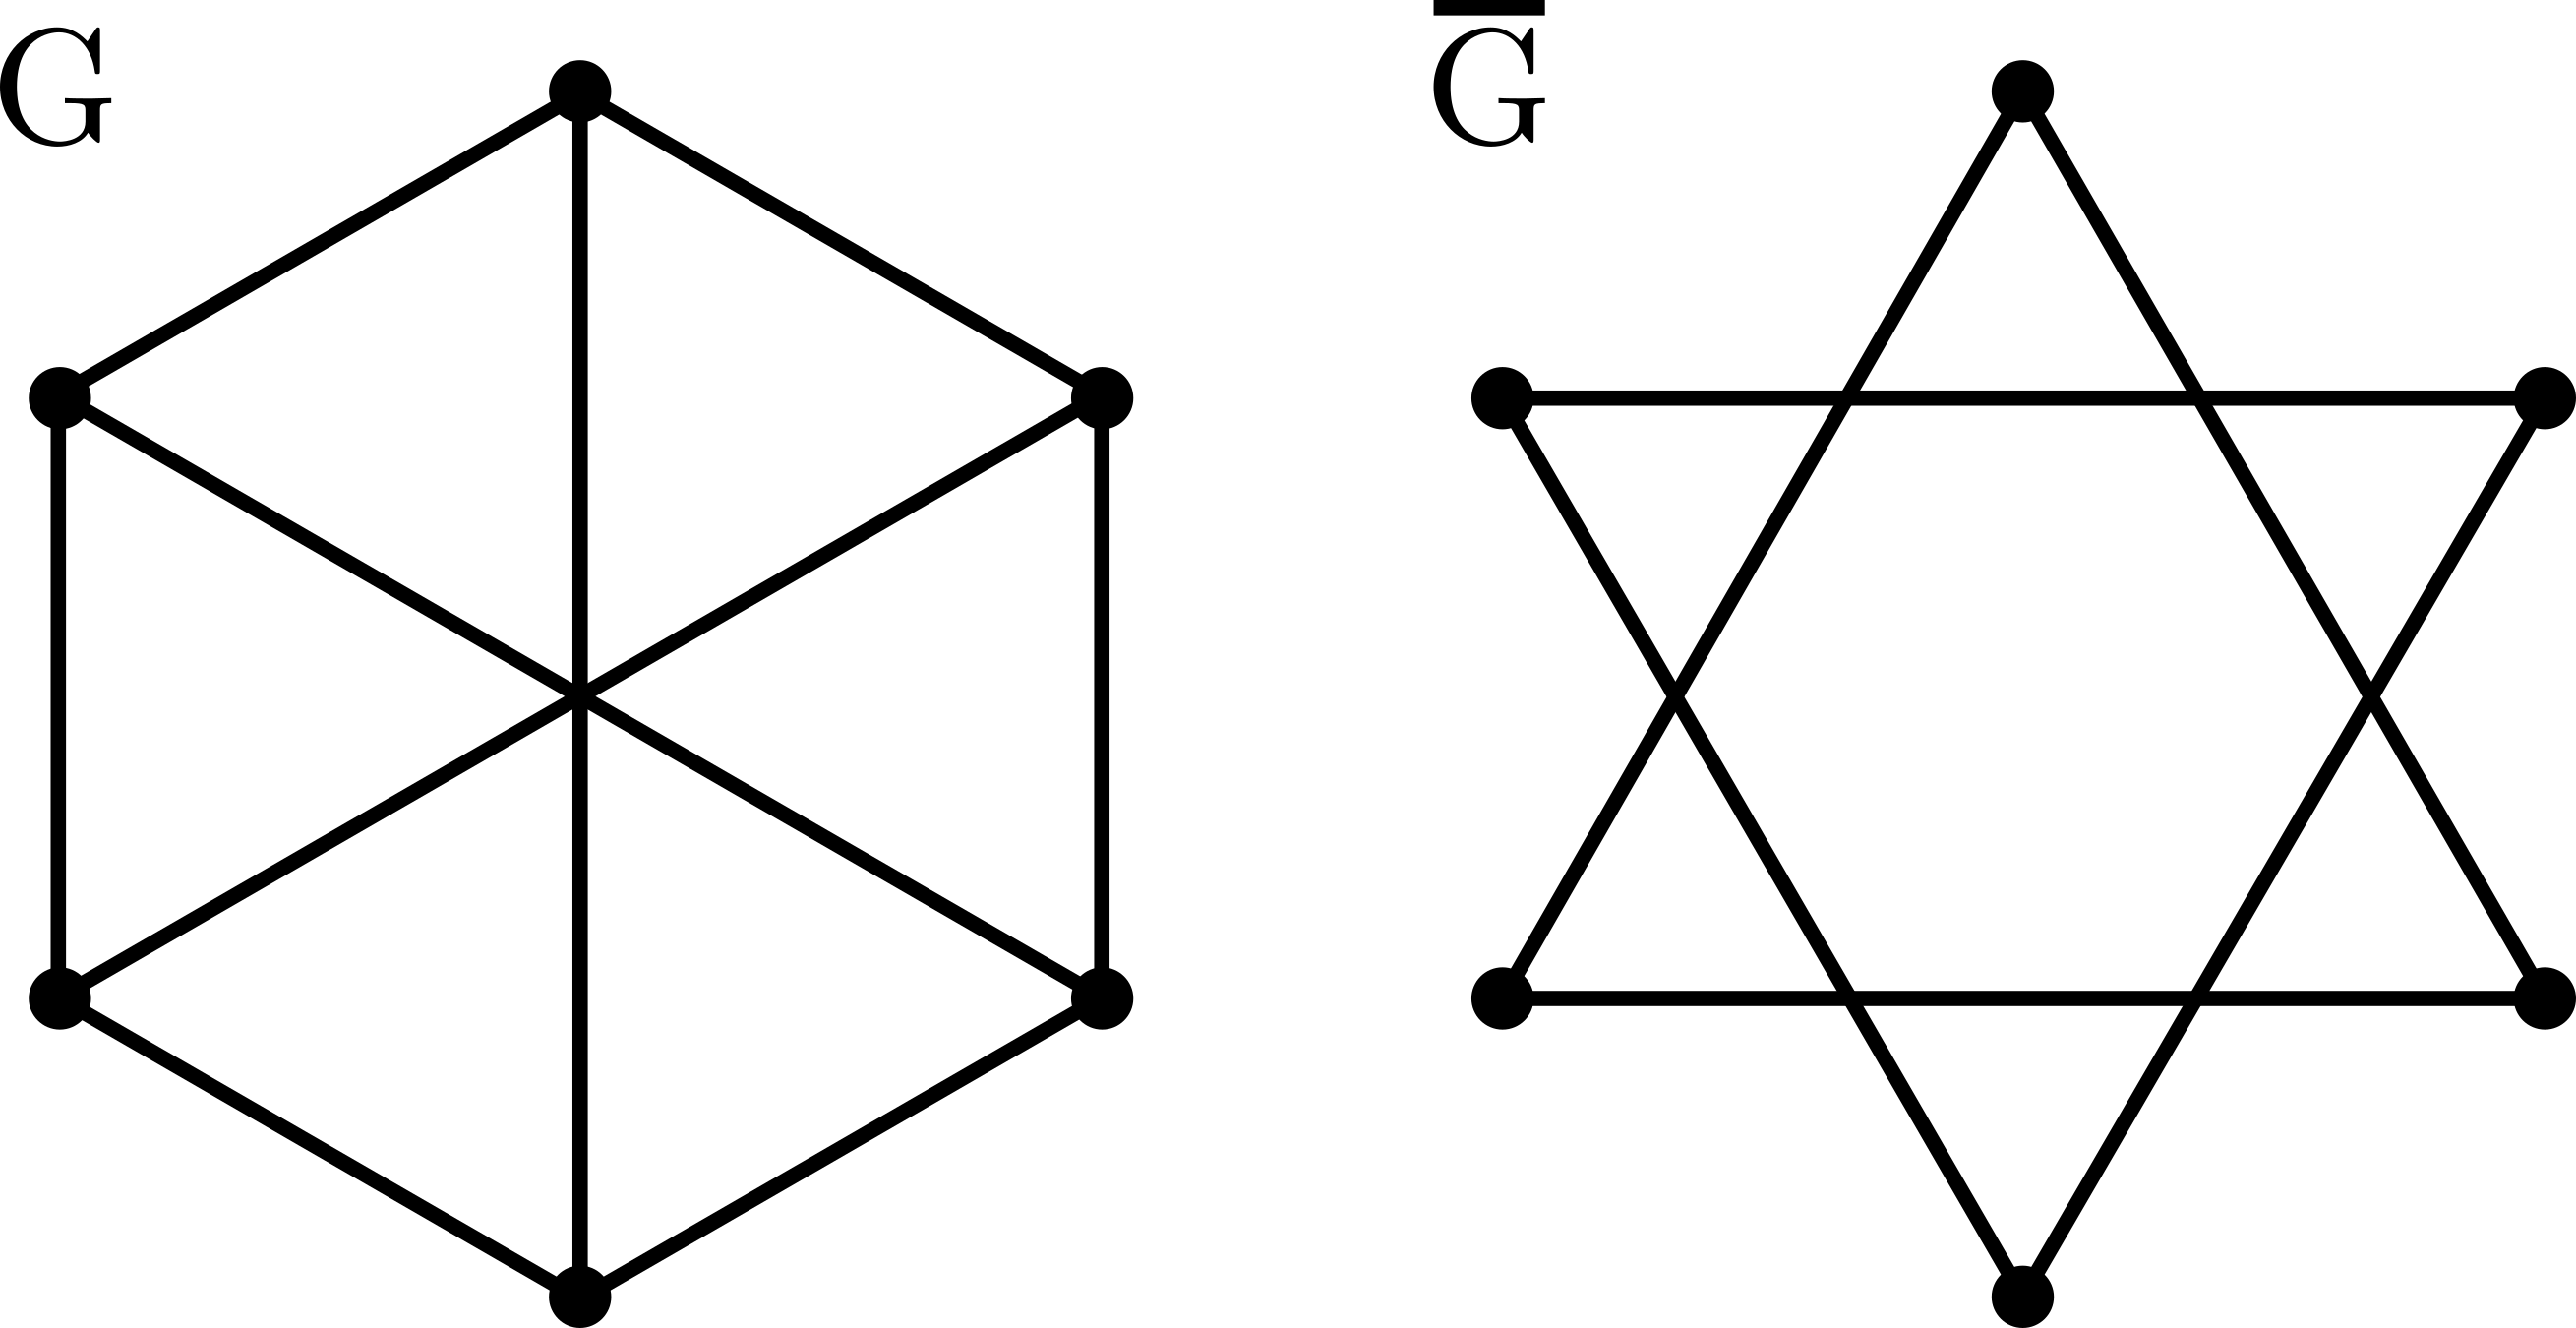
\includegraphics[width=0.65\textwidth]{images/complement-graph.png}
    \end{figure}
\end{example*}

\textbf{Самодополнительный граф} --- это граф, изоморфный своему дополнению.

\begin{example*}
    Следующие графы являются самодополнительными:
    \begin{figure}[H]
        \centering
        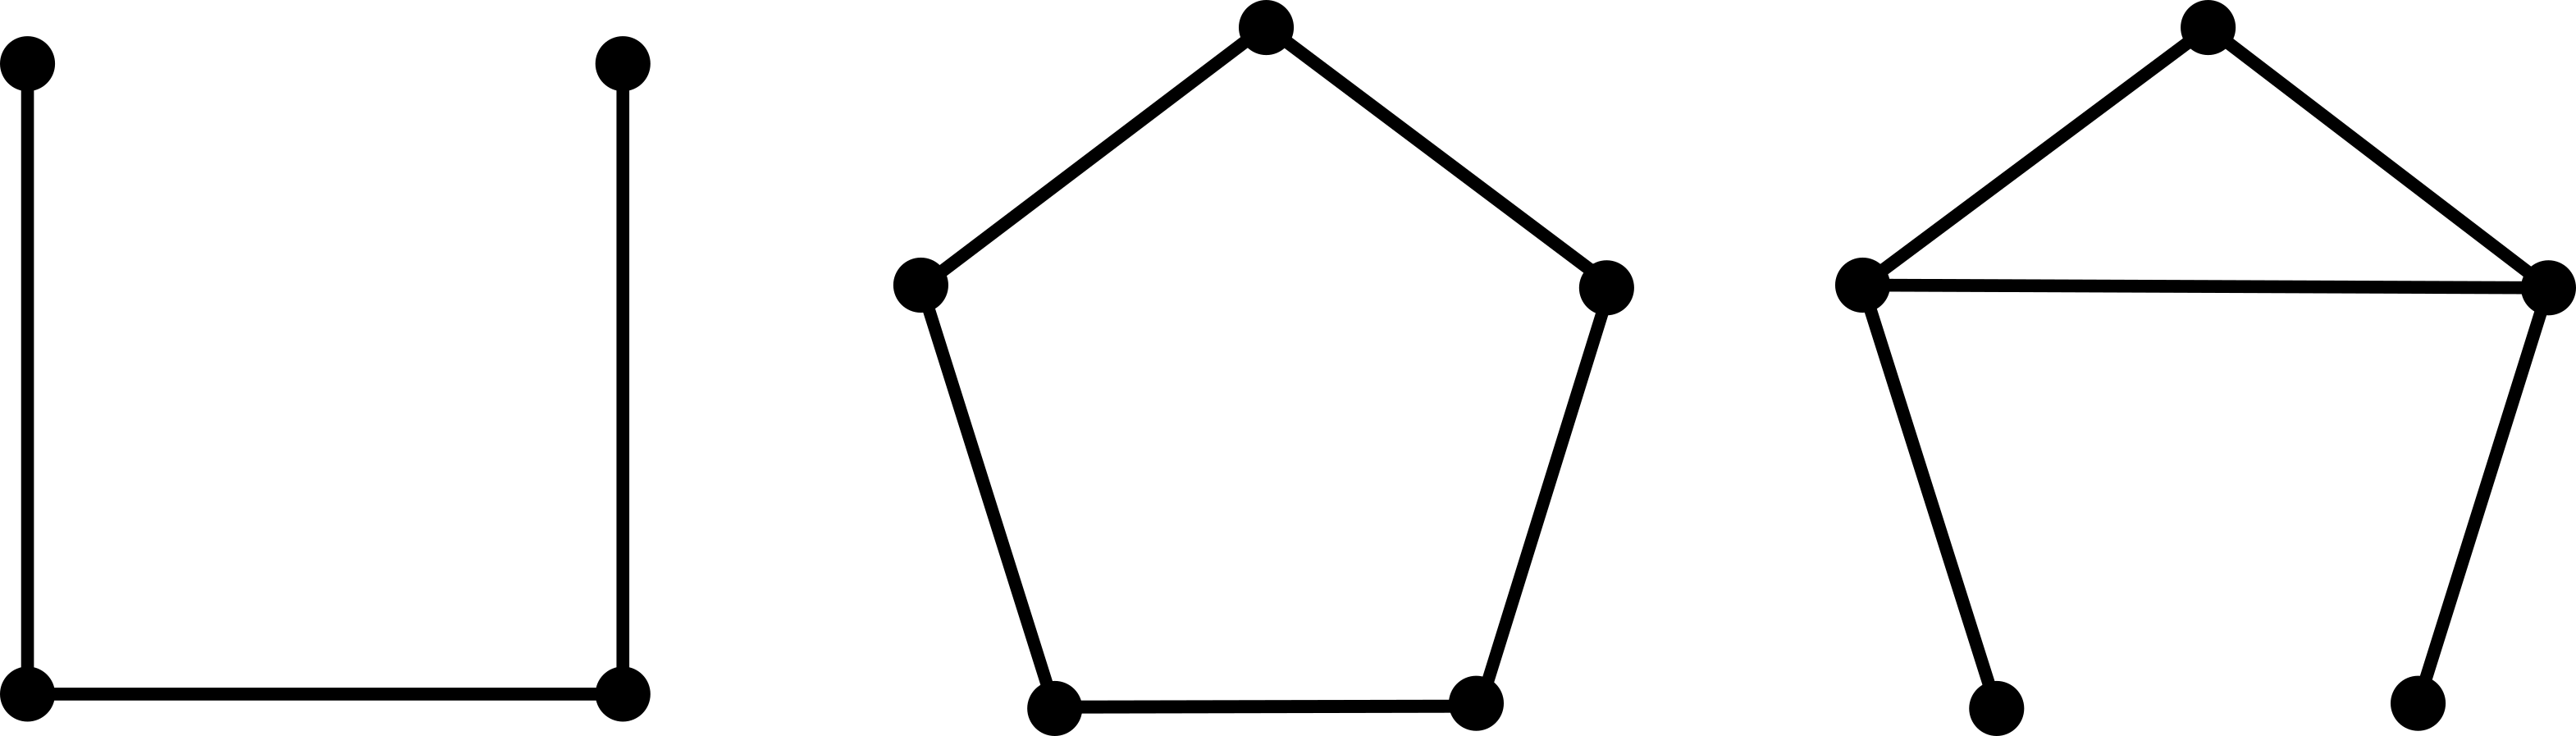
\includegraphics[width=0.8\textwidth]{images/self-complementary-graph.png}
    \end{figure}
\end{example*}

\subsection{Матричные представления графов}

Для задания графа необходимо указать два множества: \(V\) (множество вершин) и \(X\) (множество ребер или дуг). Существуют различные способы задания графов. Для алгебраического задания удобно использовать матричный способ. Выбор вида матрицы определяется конкретной задачей.

\subsubsection{Матрица смежности неориентированного графа}

Пусть мы имеем граф \(G\) с вершинами \(v_1, \ldots, v_n\) и ребрами \(x_1, \ldots, x_m\). \textbf{Матрица смежности} неориентированного простого графа \(G\) --- это квадратная матрица \(A(G)\) порядка \(n\) (\(n\) --- число вершин) с элементами
\[
    a_{ij} =
    \begin{dcases*}
        1, \text{если вершины} \; v_i \; \text{и} \; v_j \; \text{соединены ребром (смежные)}; \\
        0, \text{в противном случае}.
    \end{dcases*}
\]

Матрица смежности \(A(G)\) определяет граф \(G\) с точностью до изоморфизма, а также является симметричной матрицей с нулями по главной диагонали. Сумма элементов по строкам матрицы \(A(G)\) равна степеням вершин графа \(G\).

\begin{example*}
    Рассмотрим следующий граф:

    \begin{multicols}{2}
        \begin{center}
            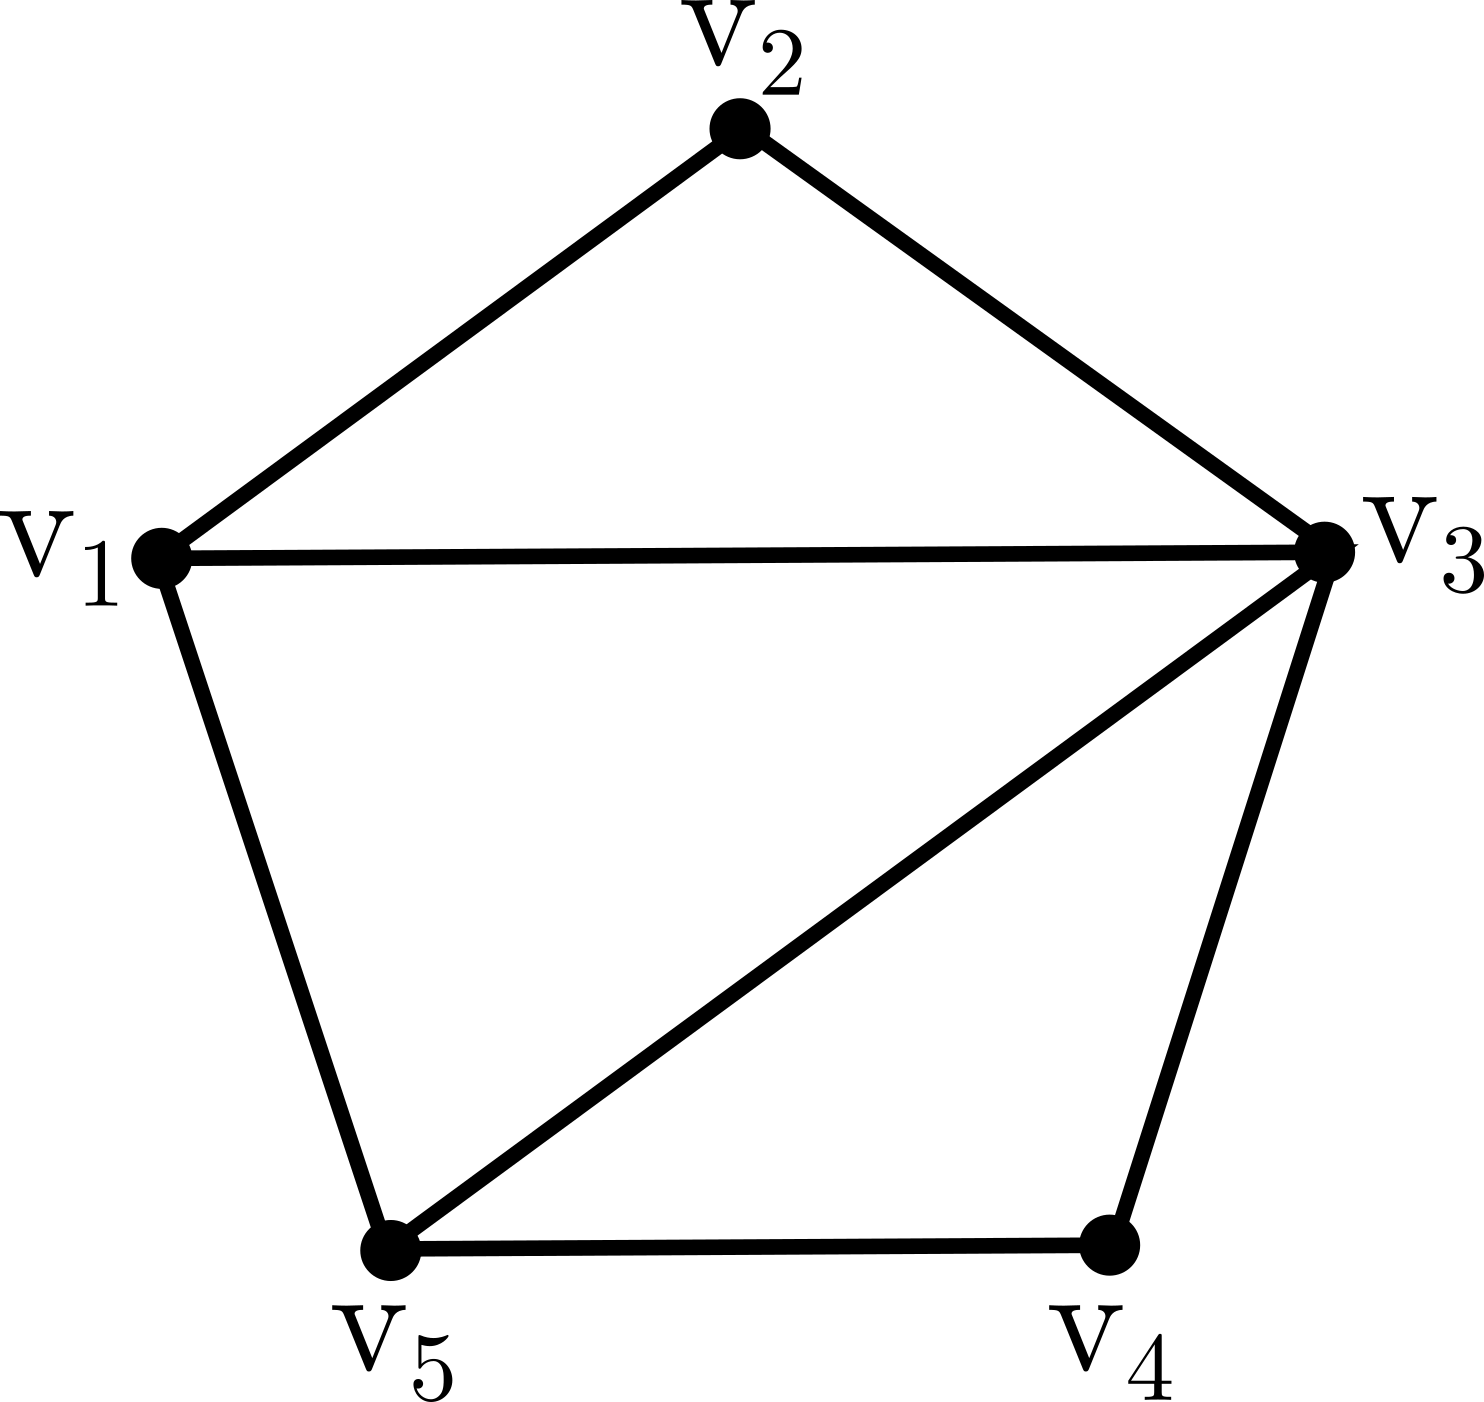
\includegraphics[width=0.45\textwidth]{images/adjacency-matrix-example.png}
        \end{center}

        \columnbreak

        \null \vfill
        \[
            A(G) =
            \begin{pmatrix}
                0 & 1 & 1 & 0 & 1 \\
                1 & 0 & 1 & 0 & 0 \\
                1 & 1 & 0 & 1 & 1 \\
                0 & 0 & 1 & 0 & 1 \\
                1 & 0 & 1 & 1 & 0
            \end{pmatrix}
        \]
        \vfill \null
    \end{multicols}

    Получили, что \(a_{12} = 1\), поскольку в графе \(G\) есть ребро, соединяющее вершины \(v_1\) и \(v_2\), и \(a_{42} = 0\), поскольку в графе \(G\) нет ребра, соединяющего вершины \(v_4\) и \(v_2\) и так далее.
\end{example*}

\subsection{Число маршрутов длины n}

Если \(A\) --- матрица смежности графа \(G\), то элемент матрицы \(A^n\), стоящий в \(i\)-й строке и \(j\)-м столбце, будет равен \textbf{числу маршрутов} длины \(n\) из вершины \(v_i\) в вершину \(v_j\).

\begin{example*}
    Рассмотрим следующий граф:

    \begin{multicols}{2}
        \null \vfill
        \begin{center}
            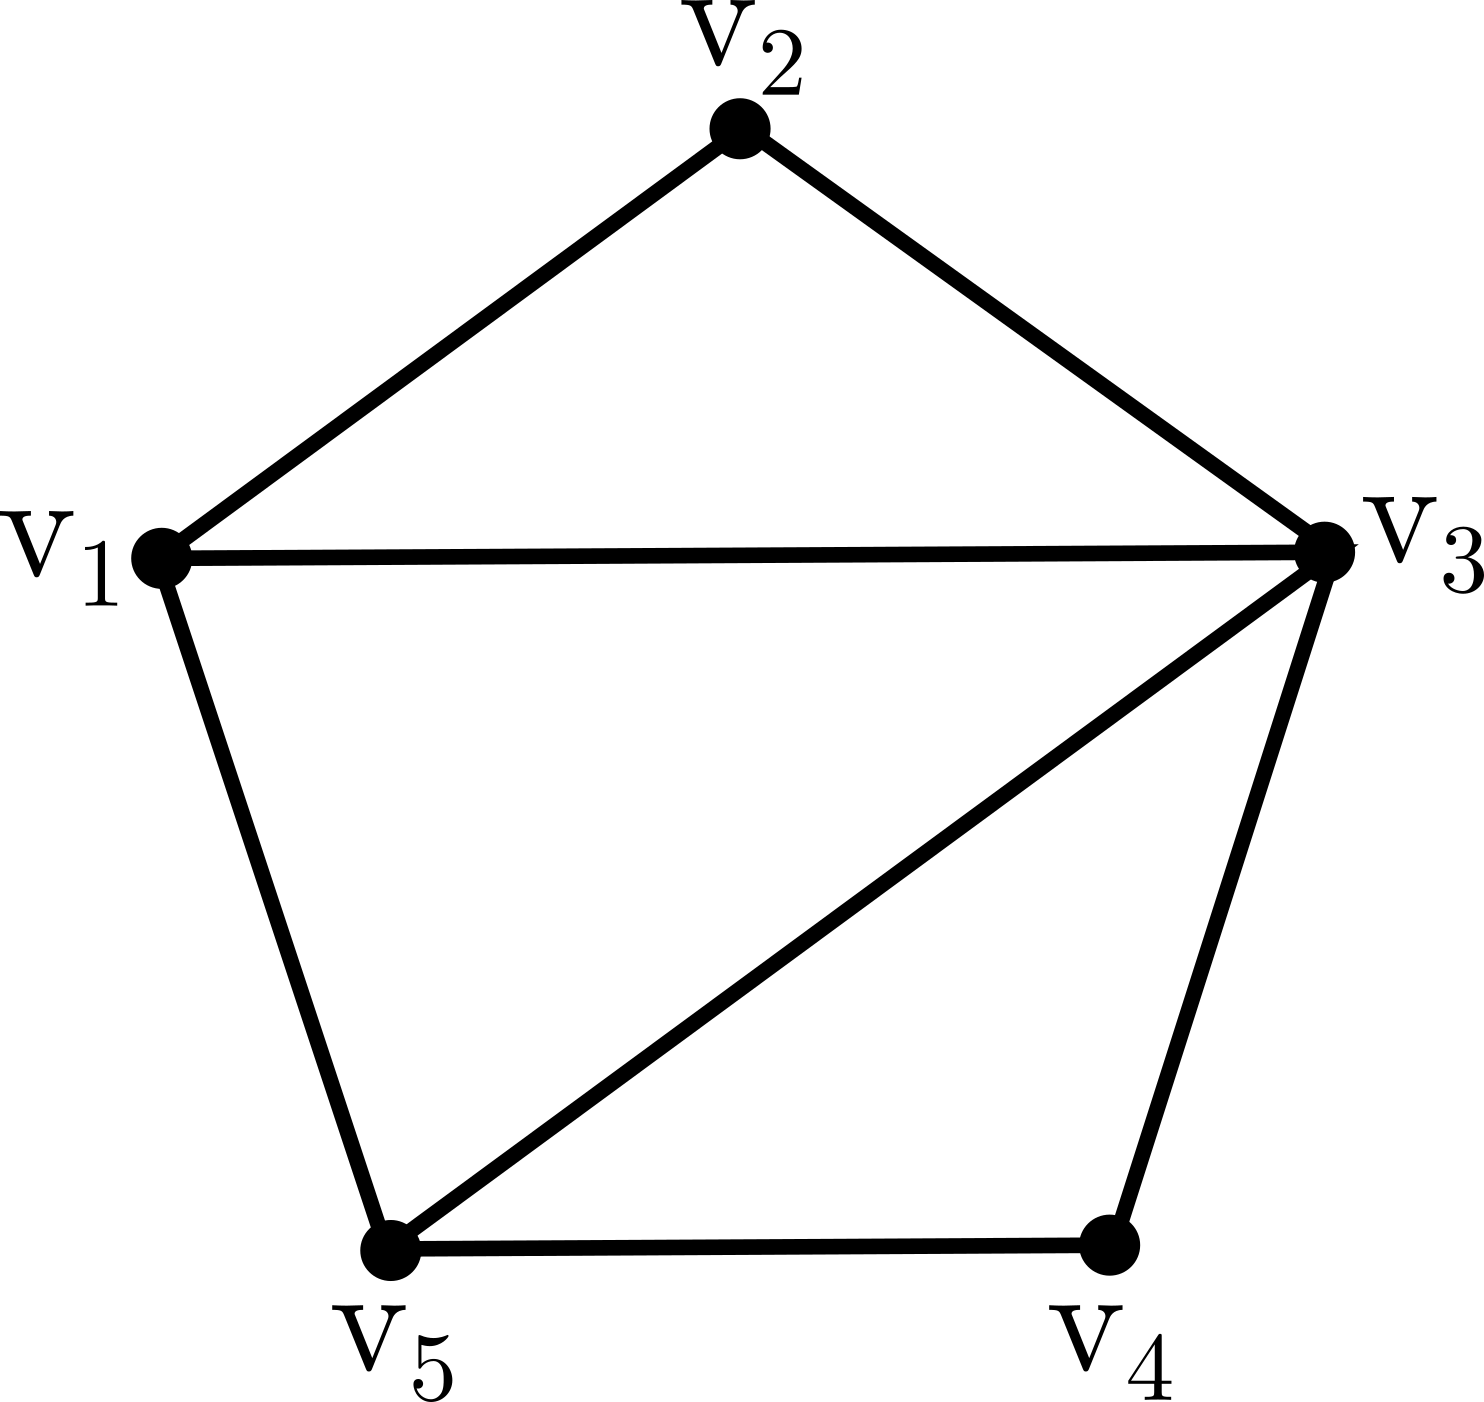
\includegraphics[width=0.45\textwidth]{images/adjacency-matrix-example.png}
        \end{center}
        \vfill \null

        \columnbreak

        \[
            A^2 =
            \begin{pmatrix}
                3 & 1 & 2 & 2 & 1 \\
                1 & 2 & 1 & 1 & 2 \\
                2 & 1 & 4 & 1 & 2 \\
                2 & 1 & 1 & 2 & 1 \\
                1 & 2 & 2 & 1 & 3
            \end{pmatrix}
        \]
        \[
            A^3 =
            \begin{pmatrix}
                4 & 5 & 7 & 3 & 7 \\
                5 & 2 & 6 & 3 & 3 \\
                7 & 6 & 6 & 6 & 7 \\
                3 & 3 & 6 & 2 & 5 \\
                7 & 3 & 7 & 5 & 4
            \end{pmatrix}
        \]
    \end{multicols}

    \noindent Существует \(2\) маршрута длины \(2\) из вершины \(v_2\) в вершину \(v_5\):
    \begin{enumerate}
        \item \(v_2\)-\(v_1\)-\(v_5\);
        \item \(v_2\)-\(v_3\)-\(v_5\).
    \end{enumerate}

    \noindent Существует \(7\) маршрутов длины \(3\) из вершины \(v_5\) в вершину \(v_3\):
    \vspace*{-1em}
    \begin{multicols}{2}
        \begin{enumerate}
            \item \(v_5\)-\(v_1\)-\(v_2\)-\(v_3\);
            \item \(v_5\)-\(v_1\)-\(v_5\)-\(v_3\);
            \item \(v_5\)-\(v_4\)-\(v_5\)-\(v_3\);
            \item \(v_5\)-\(v_3\)-\(v_5\)-\(v_3\);
            \item \(v_5\)-\(v_3\)-\(v_1\)-\(v_3\);
            \item \(v_5\)-\(v_3\)-\(v_2\)-\(v_3\);
            \item \(v_5\)-\(v_3\)-\(v_4\)-\(v_3\).
        \end{enumerate}
    \end{multicols}
\end{example*}

\subsection{Матрица смежности ориентированного графа}

Матрицей смежности орграфа \(D\) называется квадратная матрица \(A(D)\) порядка \(n\) (\(n\) --- число вершин) с элементами:
\[
    a_{ij} =
    \begin{dcases*}
        1, \text{если в орграфе} \; D \text{есть дуга из} i-\text{й} \; \text{вершины в} \; j-\text{ю} \text{вершину}; \\
        0, \text{в противном случае}.
    \end{dcases*}
\]
Матрица смежности орграфа в общем случае не будет симметричной.

\begin{example*}
    Рассмотрим следующий граф:

    \begin{figure}[H]
        \centering
        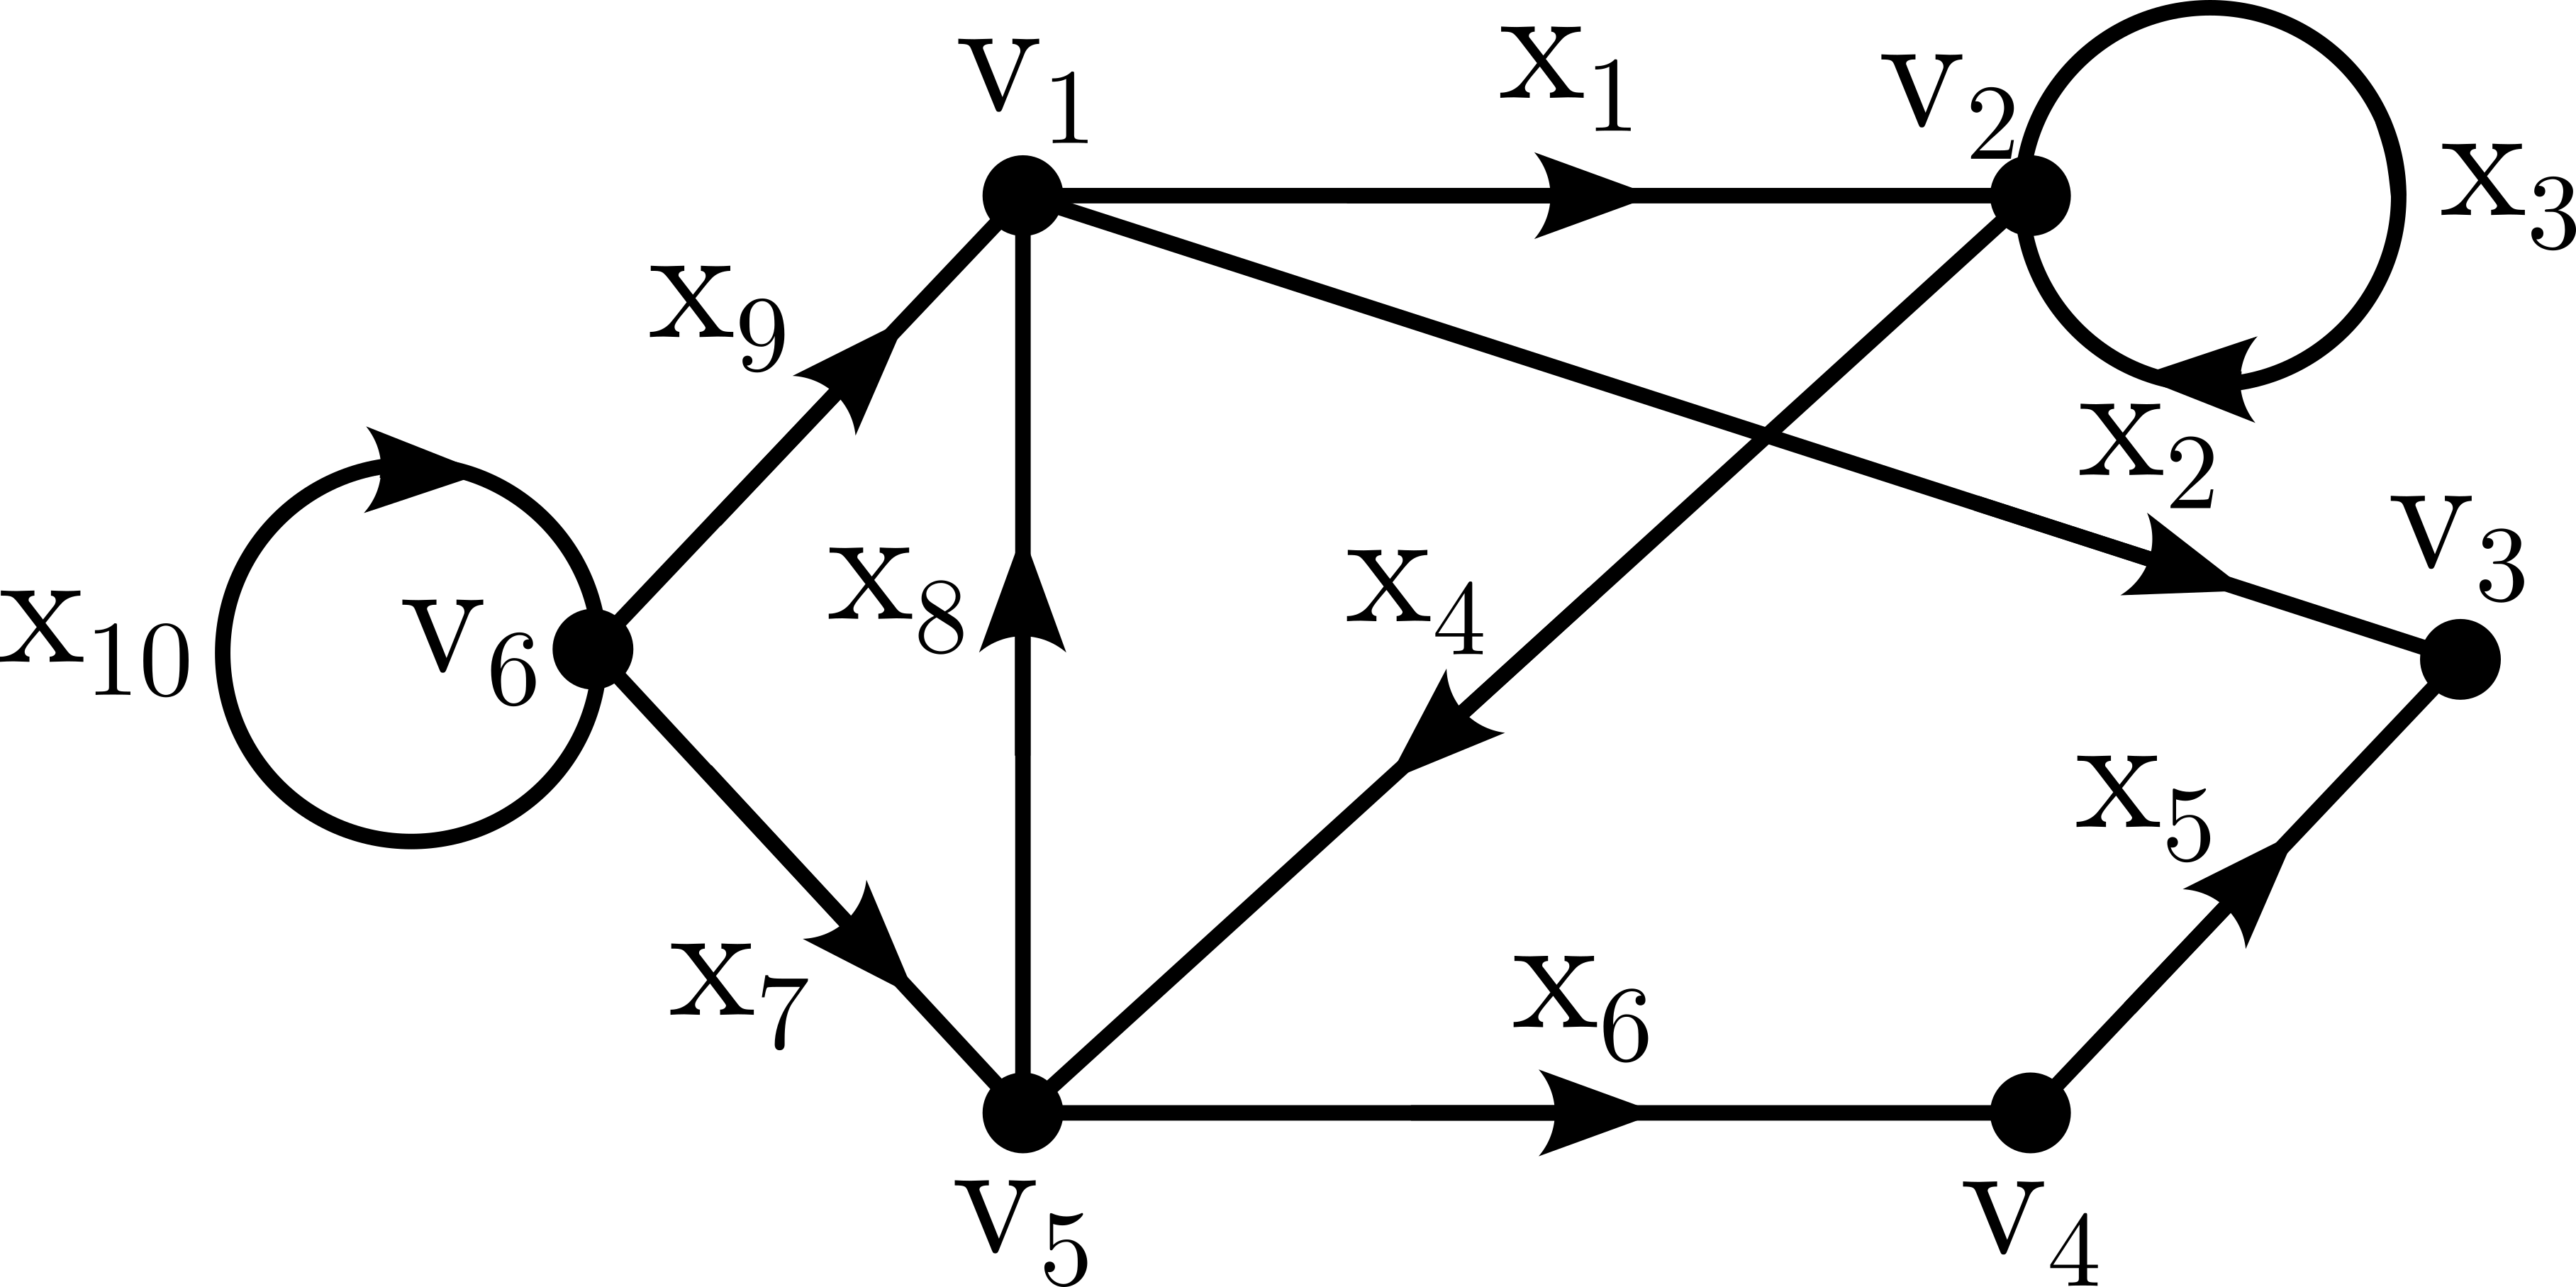
\includegraphics[width=0.8\textwidth]{images/directed-graph-example.png}
    \end{figure}

    \[
        A(D) =
        \begin{pmatrix}
            0 & 1 & 1 & 0 & 0 & 0 \\
            0 & 1 & 0 & 0 & 1 & 0 \\
            0 & 0 & 0 & 0 & 0 & 0 \\
            0 & 0 & 1 & 0 & 0 & 0 \\
            1 & 0 & 0 & 1 & 0 & 0 \\
            1 & 0 & 0 & 0 & 1 & 1
        \end{pmatrix}
    \]

    Сумма всех элементов \(i\)-й строки равна числу дуг, выходящий из вершины \(v_i\). Сумма всех элементов \(j\)-го столбца равен числу дуг, направленных в вершину \(v_j\). Если \(A\) --- матрица смежности орграфа \(D\), то
    элемент матрицы \(A^n\), стоящий в \(i\)-й строке и \(j\)-м столбце, будет равен числу путей (не обязательно оргцепей и простых оргцепей) длины \(n\), идущих из вершины \(v_i\) в вершину \(v_j\).
\end{example*}

\subsection{Матрица инцидентности неориентированного графа}

\textbf{Матрицей инцидентности} графа \(G\) называется матрица размера \(n \times m\) такая, что \(B(G) = (b_{ij})\), где
\[
    b_{ij} =
    \begin{dcases*}
        1, \text{если вершина} \; v_i \; \text{инцидентна ребру} \; x_j, \\
        0, \text{в противом случае}.
    \end{dcases*}
\]
Матрица \(B(G)\) определяет граф \(G\) с точностью до изоморфизма.

\begin{example*}
    Рассмотрим следующий граф:

    \begin{multicols}{2}
        \begin{center}
            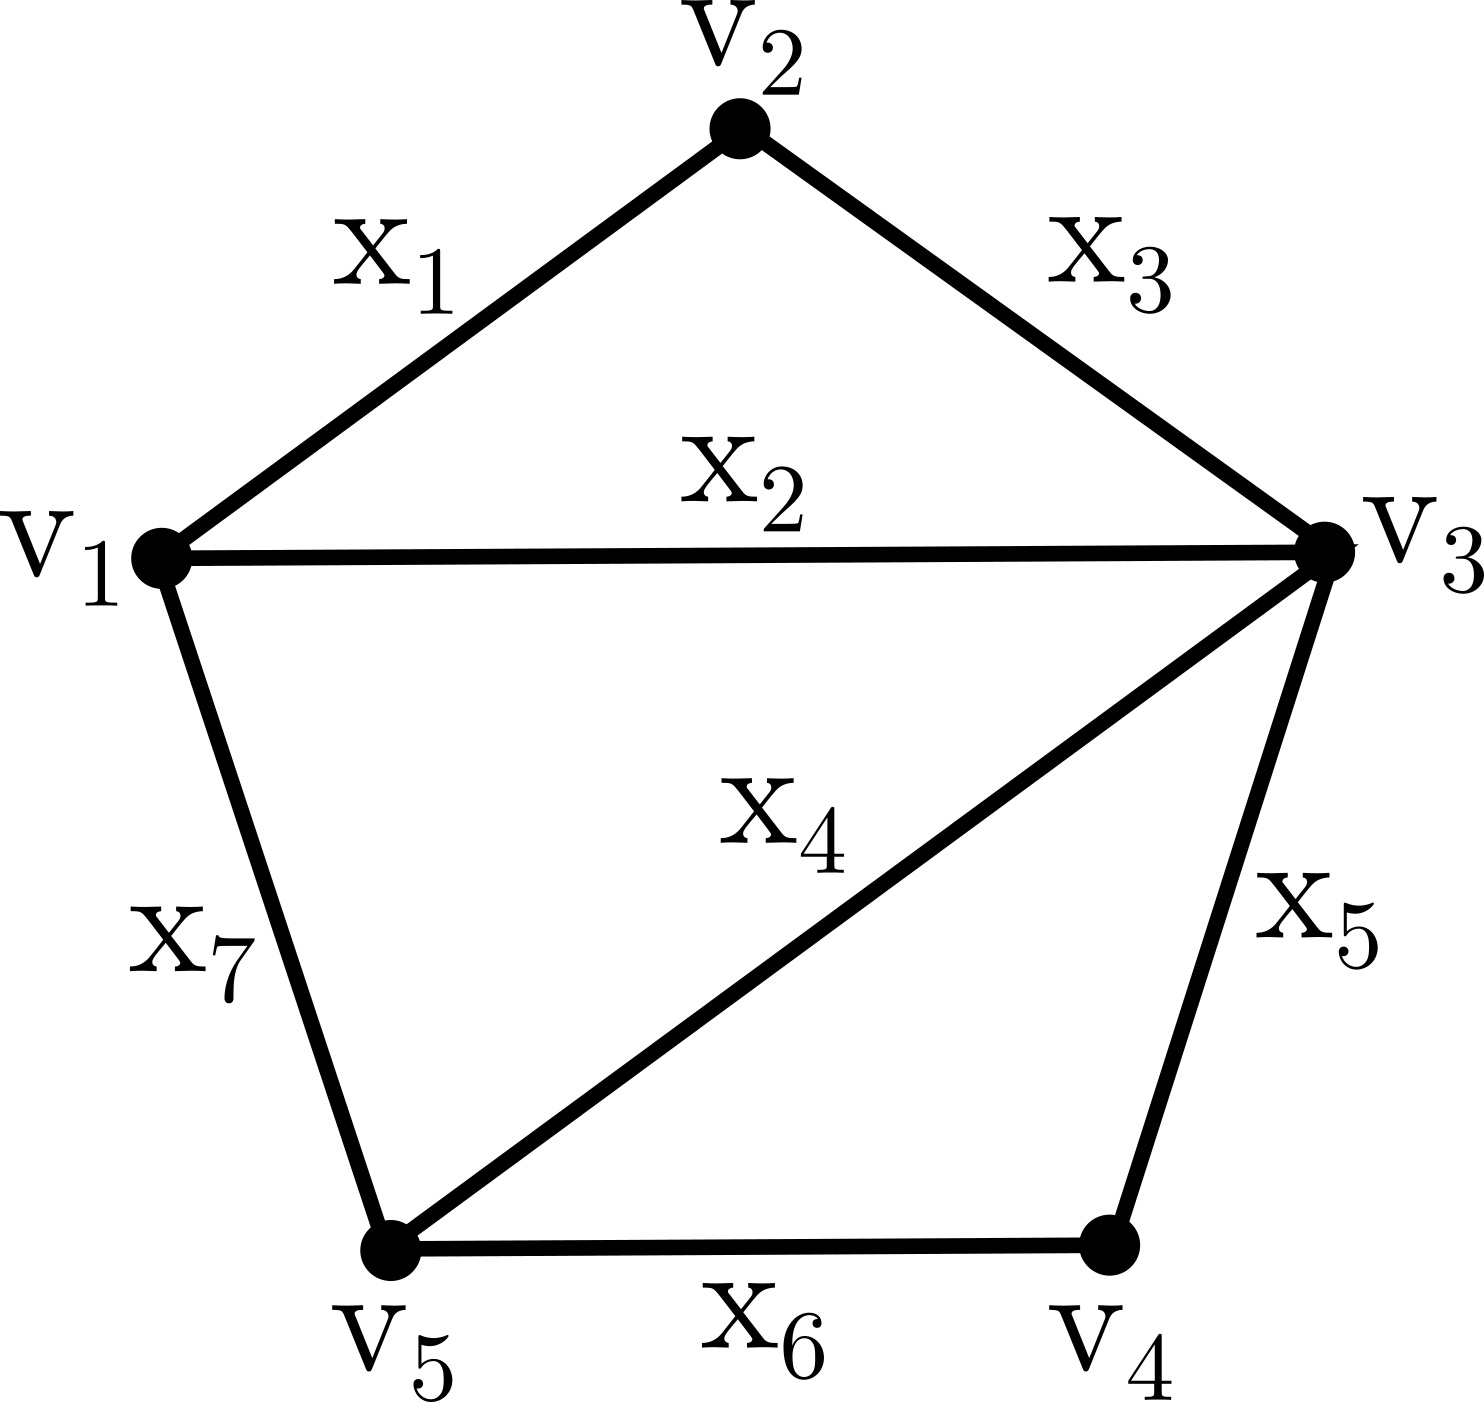
\includegraphics[width=0.45\textwidth]{images/incidence-matrix-example.png}
        \end{center}

        \columnbreak

        \null \vfill
        \[
            B(G) =
            \begin{pmatrix}
                1 & 1 & 0 & 0 & 0 & 0 & 1 \\
                1 & 0 & 1 & 0 & 0 & 0 & 0 \\
                0 & 1 & 1 & 1 & 1 & 0 & 0 \\
                0 & 0 & 0 & 0 & 1 & 1 & 0 \\
                0 & 0 & 0 & 1 & 0 & 1 & 1
            \end{pmatrix}
        \]
        \vfill \null
    \end{multicols}
\end{example*}

\subsection{Ациклический граф}

Граф называется \textbf{ациклическим}, если в нем нет циклов. \textbf{Дерево} --- это связный ациклический граф. В любом нетривиальном дереве имеется по крайней мере две висячие вершины.

Каждый граф, не содержащий циклов, называется \textbf{лесом}. Компонентами леса являются деревья.

\subsection{Деревья}

Граф \(G = (V, E)\) называется \textbf{деревом}, если он связен и ацикличен (то есть не содержит циклов).

Пусть \(G = (V, E)\) --- граф с \(n\) вершинами и \(m\) ребрами. Тогда следующие условия будут необходимыми и достаточными, чтобы граф \(G\) являлся деревом:
\begin{itemize}
    \item любая пара вершин в \(G\) соединена единственным путем;
    \item \(G\) связен и \(m = n - 1\);
    \item \(G\) связен, а удаление хотя бы одного его ребра нарушает связность графа;
    \item \(G\) ацикличен, но если добавить хотя бы одно ребро, то в \(G\) появится цикл.
\end{itemize}

\subsection{Дерево с корнем}

\textbf{Деревом с корнем} называется дерево с одной выделенной вершиной. Эта выделанная вершина и является \textbf{корнем} дерева. Вершины дерева, лежащие непосредственно под данной, называются \textbf{сыновьями}. С другой стороны, вершина, стоящая непосредственно перед сыном, называется ее \textbf{отцом}. Вершины, которые не имеют сыновей, принято называть \textbf{листьями}. Остальные вершины, отличные от корня и листьев, называют \textbf{внутренними}.

\subsection{Бинарные деревья с корнем}

\textbf{Двоичное дерево} --- это дерево, у которого каждая его вершина имеет не более двух сыновей. В двоичном дереве с корнем вниз от каждой вершины идет не более двух ребер. Вершины степени \(1\) будем называть \textbf{концевыми}.

\begin{theorem*}
    Количество бинарных деревьев с \(n\) концевыми вершинами равно \(C(n - 1)\).
\end{theorem*}

\subsection{Остовное дерево}

В любом связном графе найдется подграф, являющимся деревом. Подграф в \(G\), являющийся деревом и включающий в себя все вершины \(G\), называется \textbf{остовным деревом}.

Остовное дерево в графе \(G\) строится просто: выбираем произвольное его ребро и последовательно добавляем другие ребра, не создавая при этом циклов, до тех пор, пока нельзя будет добавить никакого ребра, не получив при этом цикла.

Для построения остовного дерева в графе из \(n\) вершин необходимо выбрать ровно \(n - 1\) ребро.

\subsection{Нахождение минимального остовного дерева}

Существует несколько алгоритмов нахождения минимального остовного дерева. Мы рассмотрим алгоритм Краскала и алгоритм Прима.

\textbf{Алгоритм Краскала}. Выбираем ребро с наименьшим весом. Далее, к полученному подграфу добавляем наименьшее ребро (не обязательно смежное), не образующее с ним цикла. Продолжаем до тех пор, пока все вершины не будут включены в дерево.

\textbf{Алгоритм Прима}. Выбираем любую вершину графа, от нее ищем смежное ребро с наименьшим весом. Далее, уже к построенному поддереву присоединяем следующее смежное ребро наименьшего веса, не образующее с ним цикла. Продолжаем до тех пор, пока все вершины не будут включены в дерево.

\subsection{Число остовных деревьев}

Число остовных деревьев можно найти с помощью формулы Кирхгофа. Утверждение Кирхгофа формулируется следующим образом.
\begin{theorem*}
    Число остовных деревьев в связном графе \(G\) равно любому алгебраическому дополнению матрицы
    \[
        K = D - A,
    \]
    где \(A\) --- матрица смежности графа \(G\), \(D\) --- матрица степеней графа \(G\).
\end{theorem*}

\begin{example*}
    Найти число остовных деревьев графа \(G\):

    \begin{figure}[H]
        \centering
        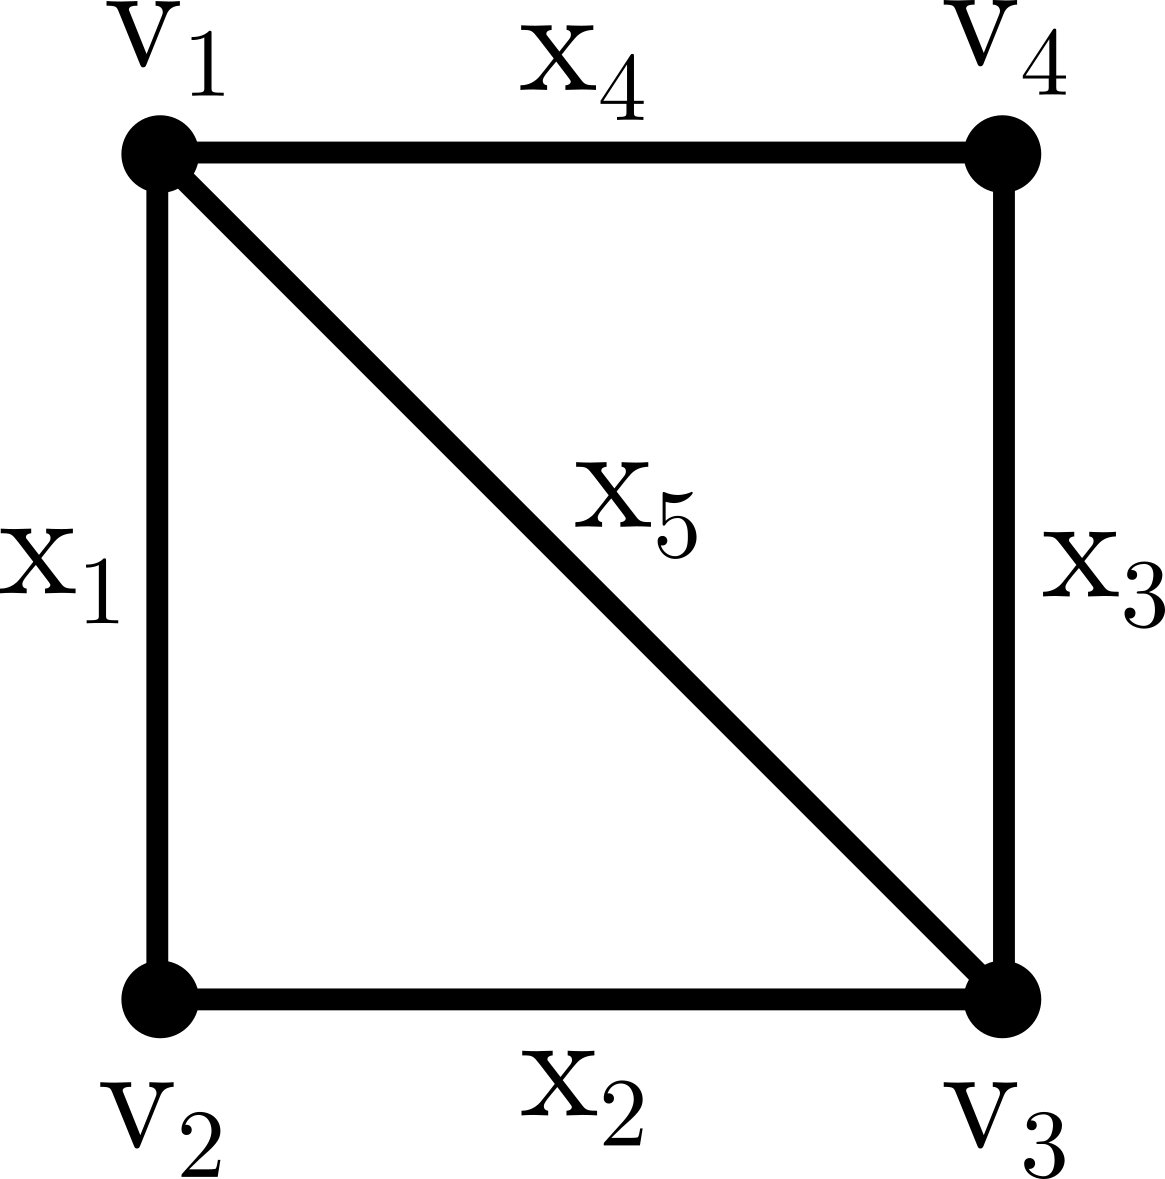
\includegraphics[width=0.35\textwidth]{images/spanning-tree-count.png}
    \end{figure}

    \[
        D =
        \begin{pmatrix}
            3 & 0 & 0 & 0 \\
            0 & 2 & 0 & 0 \\
            0 & 0 & 3 & 0 \\
            0 & 0 & 0 & 2
        \end{pmatrix}
        \qquad
        A =
        \begin{pmatrix}
            0 & 1 & 1 & 1 \\
            1 & 0 & 1 & 0 \\
            1 & 1 & 0 & 1 \\
            1 & 0 & 1 & 0
        \end{pmatrix}
    \]
    \[
        K = D - A =
        \begin{pmatrix}
            3 & 0 & 0 & 0 \\
            0 & 2 & 0 & 0 \\
            0 & 0 & 3 & 0 \\
            0 & 0 & 0 & 2
        \end{pmatrix}
        -
        \begin{pmatrix}
            0 & 1 & 1 & 1 \\
            1 & 0 & 1 & 0 \\
            1 & 1 & 0 & 1 \\
            1 & 0 & 1 & 0
        \end{pmatrix}
        =
        \begin{pmatrix}
            3  & -1 & -1 & -1 \\
            -1 & 2  & -1 & 0  \\
            -1 & -1 & 3  & -1 \\
            -1 & 0  & -1 & 2
        \end{pmatrix}
    \]
    \[
        K_{11} =
        \begin{vmatrix}
            2  & -1 & 0  \\
            -1 & 3  & -1 \\
            0  & -1 & 2
        \end{vmatrix}
        = 8.
    \]
\end{example*}

\subsection{Плоские и планарные графы}

Будем говорить, что граф \textbf{укладывается} на поверхности \(S\), если его можно нарисовать на \(S\) так, что никакие два его ребра не пересекаются.

\textbf{Планарным графом} называют граф, который можно уложить на плоскости. \textbf{Плоский граф} --- это граф, который уже уложен на плоскости.

\begin{example*}
    Левый граф планарный, правый граф плоский:
    \begin{multicols}{2}
        \centering
        \null \vfill
        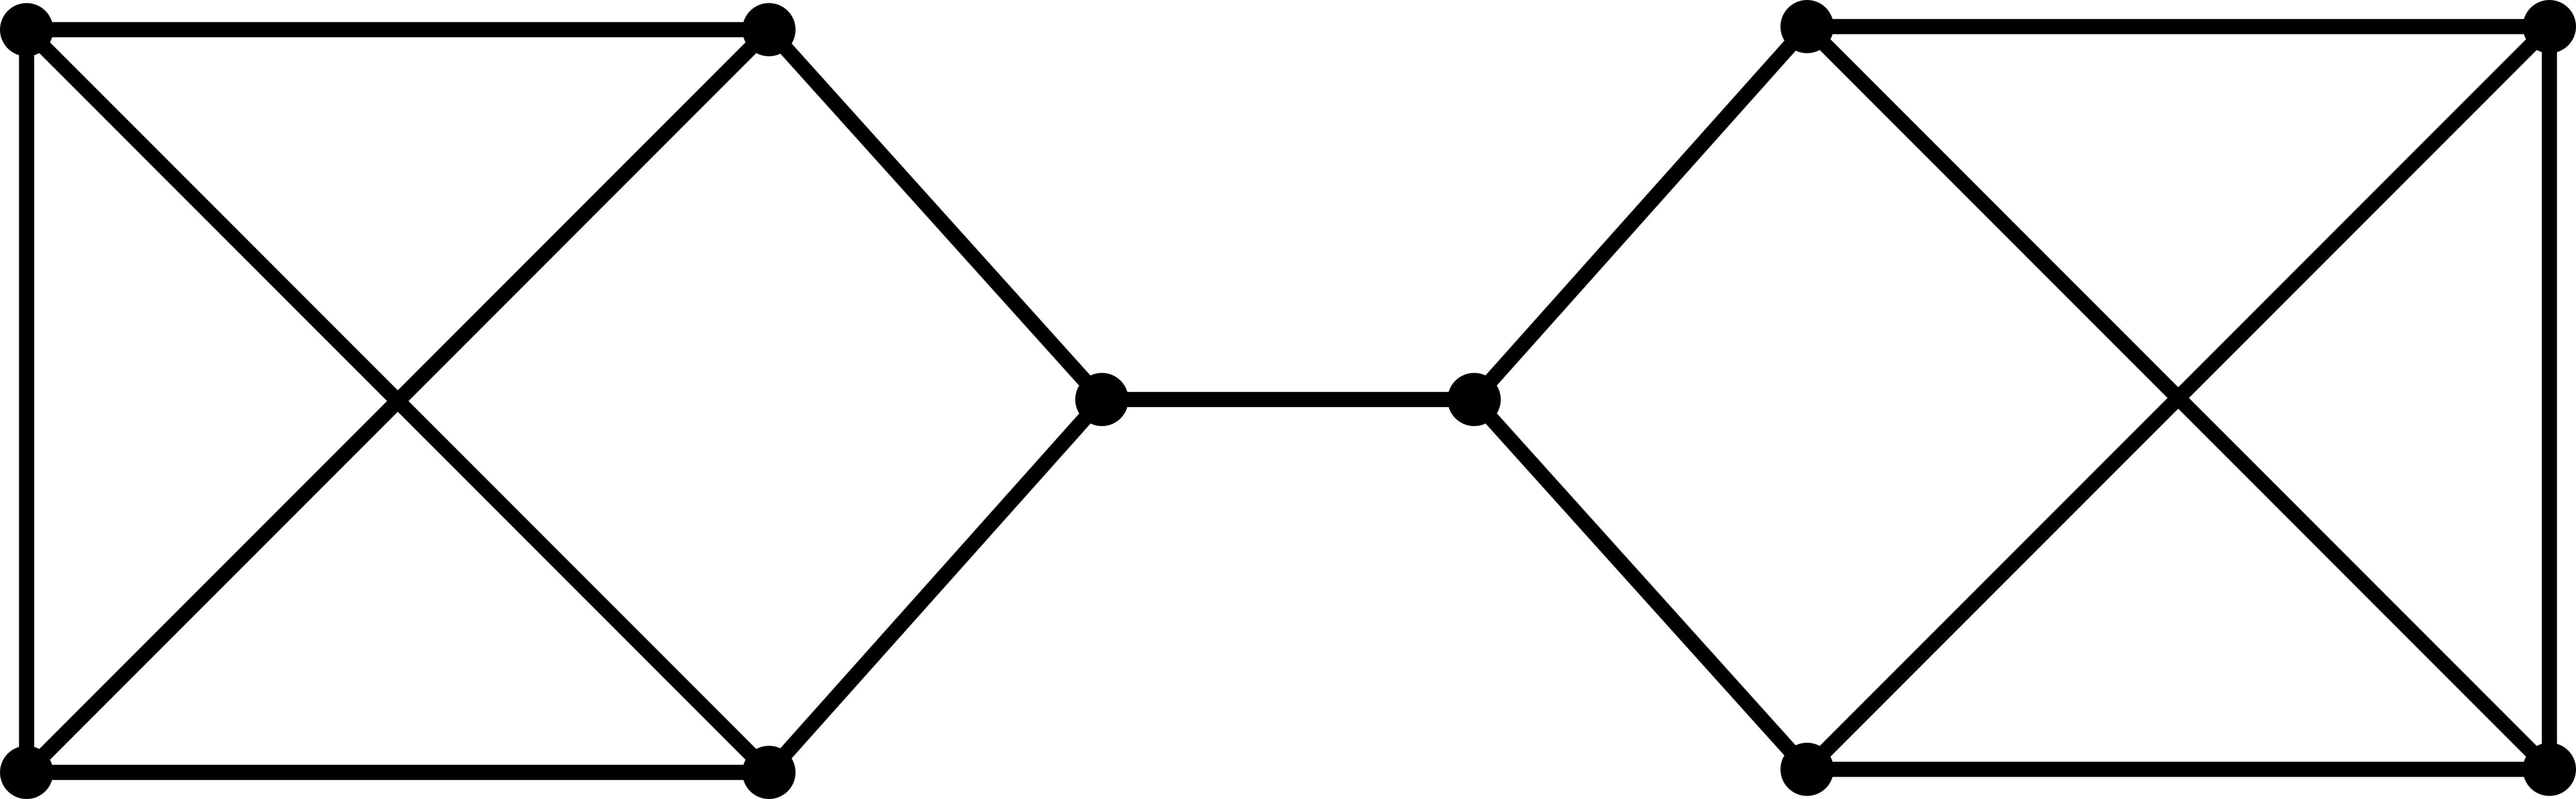
\includegraphics[width=0.45\textwidth]{images/planar-graph.png}
        \vfill \null
        \columnbreak
        \centering
        \null \vfill
        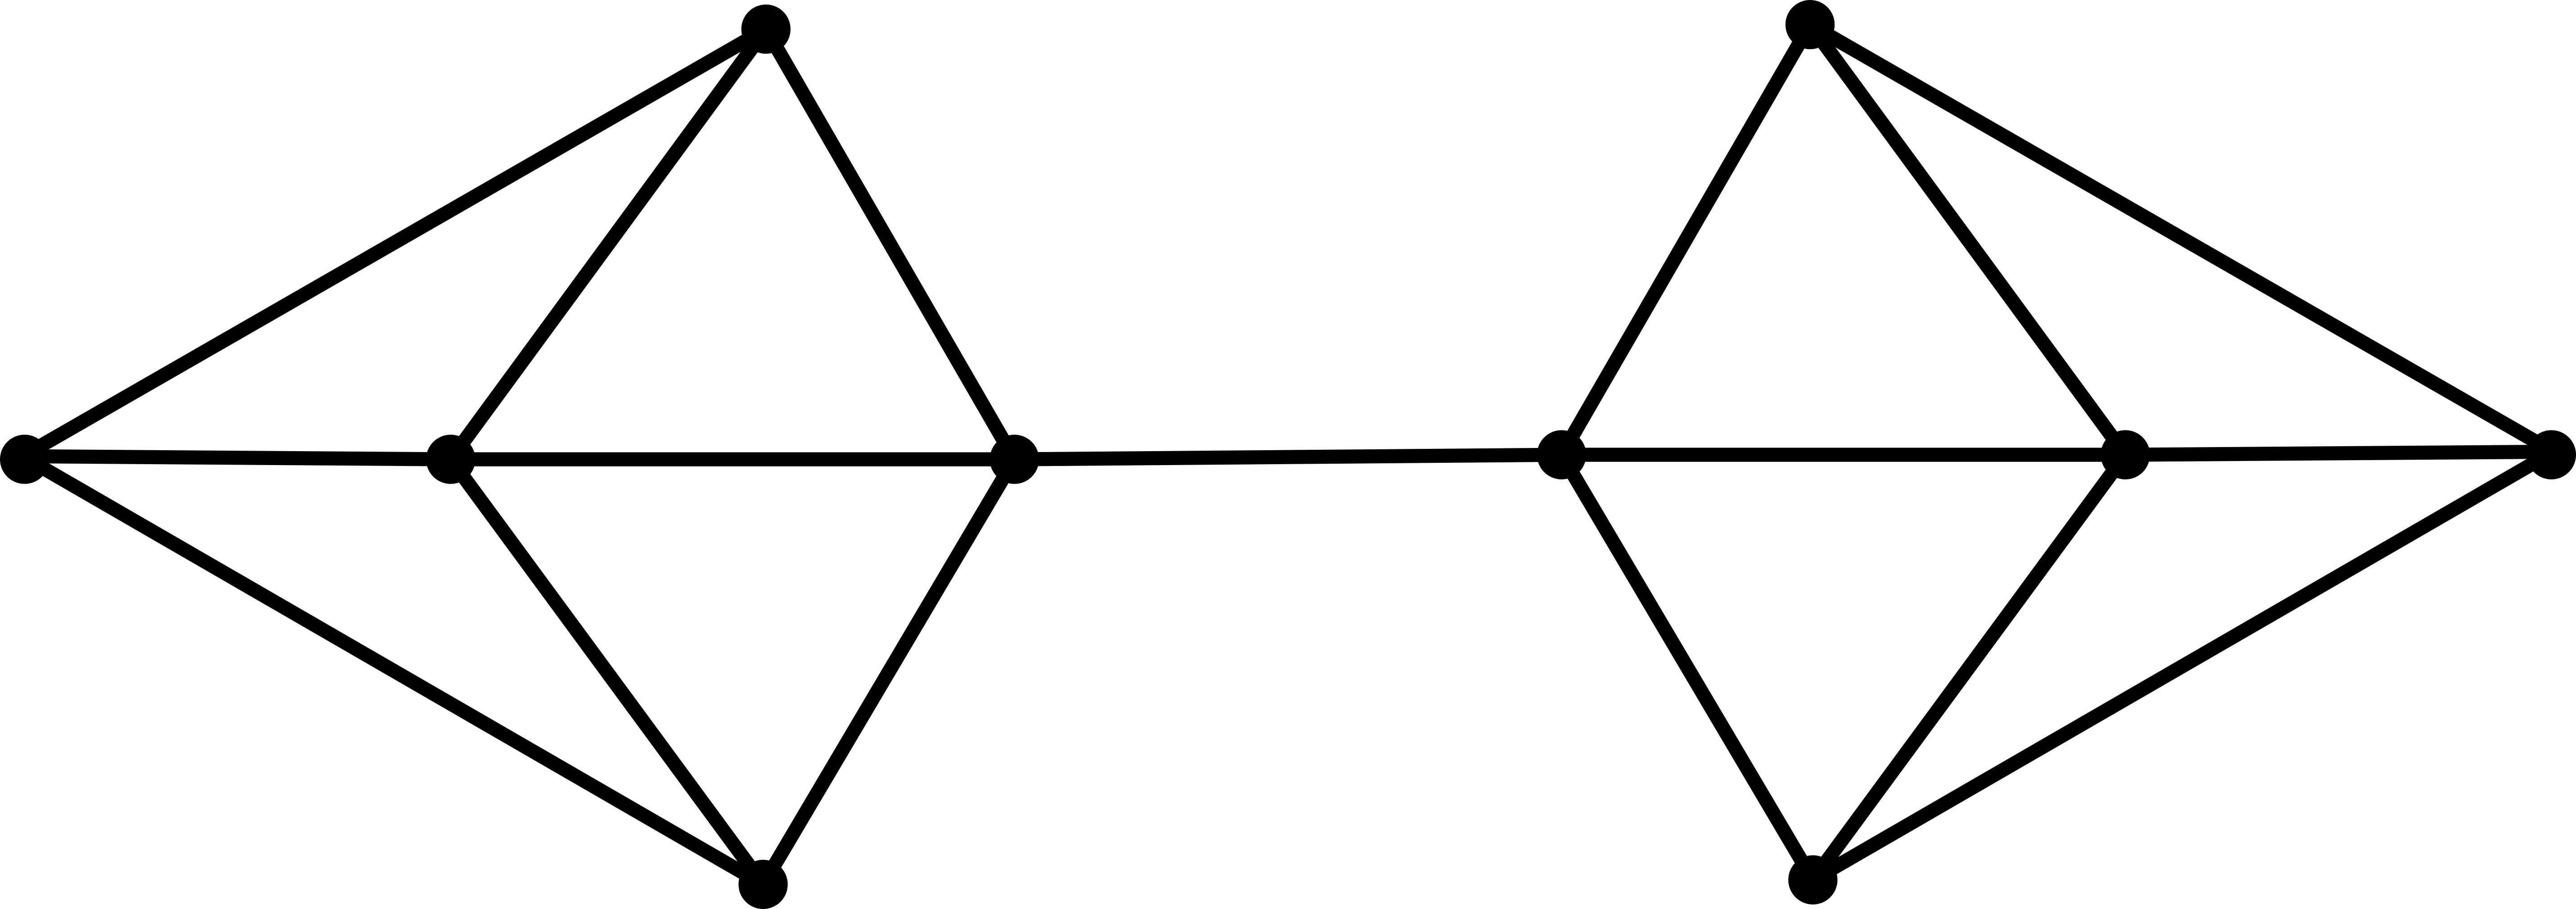
\includegraphics[width=0.45\textwidth]{images/plane-graph.png}
        \vfill \null
    \end{multicols}
\end{example*}

Области, определяемые плоским графом, называют \textbf{гранями} (или внутренними гранями). Неограниченную область называют \textbf{внешней гранью}.

\begin{theorem*}[формула Эйлера]
    Для плоского графа, имеющего \(n\) вершин, \(m\) ребер и \(f\) граней, справедлива формула
    \[
        n - m + f = 2.
    \]
\end{theorem*}

\textbf{Элементарное стягивание} в графе \(G\) (или стягивание ребра) получается отождествлением двух смежных вершин \(u\) и \(v\), то есть удалением \(u\) и \(v\) и добавлением новой вершины \(w\), смежной с теми вершинами графа, которые были смежны или с \(u\), или с \(v\).

Граф \(G\) называется \textbf{стягиваемым} к графу \(H\), если \(H\) можно получить из \(G\) с помощью некоторой последовательности элементарных стягиваний.

\begin{example*}
    Рассмотрим следующие графы:
    \begin{figure}[H]
        \centering
        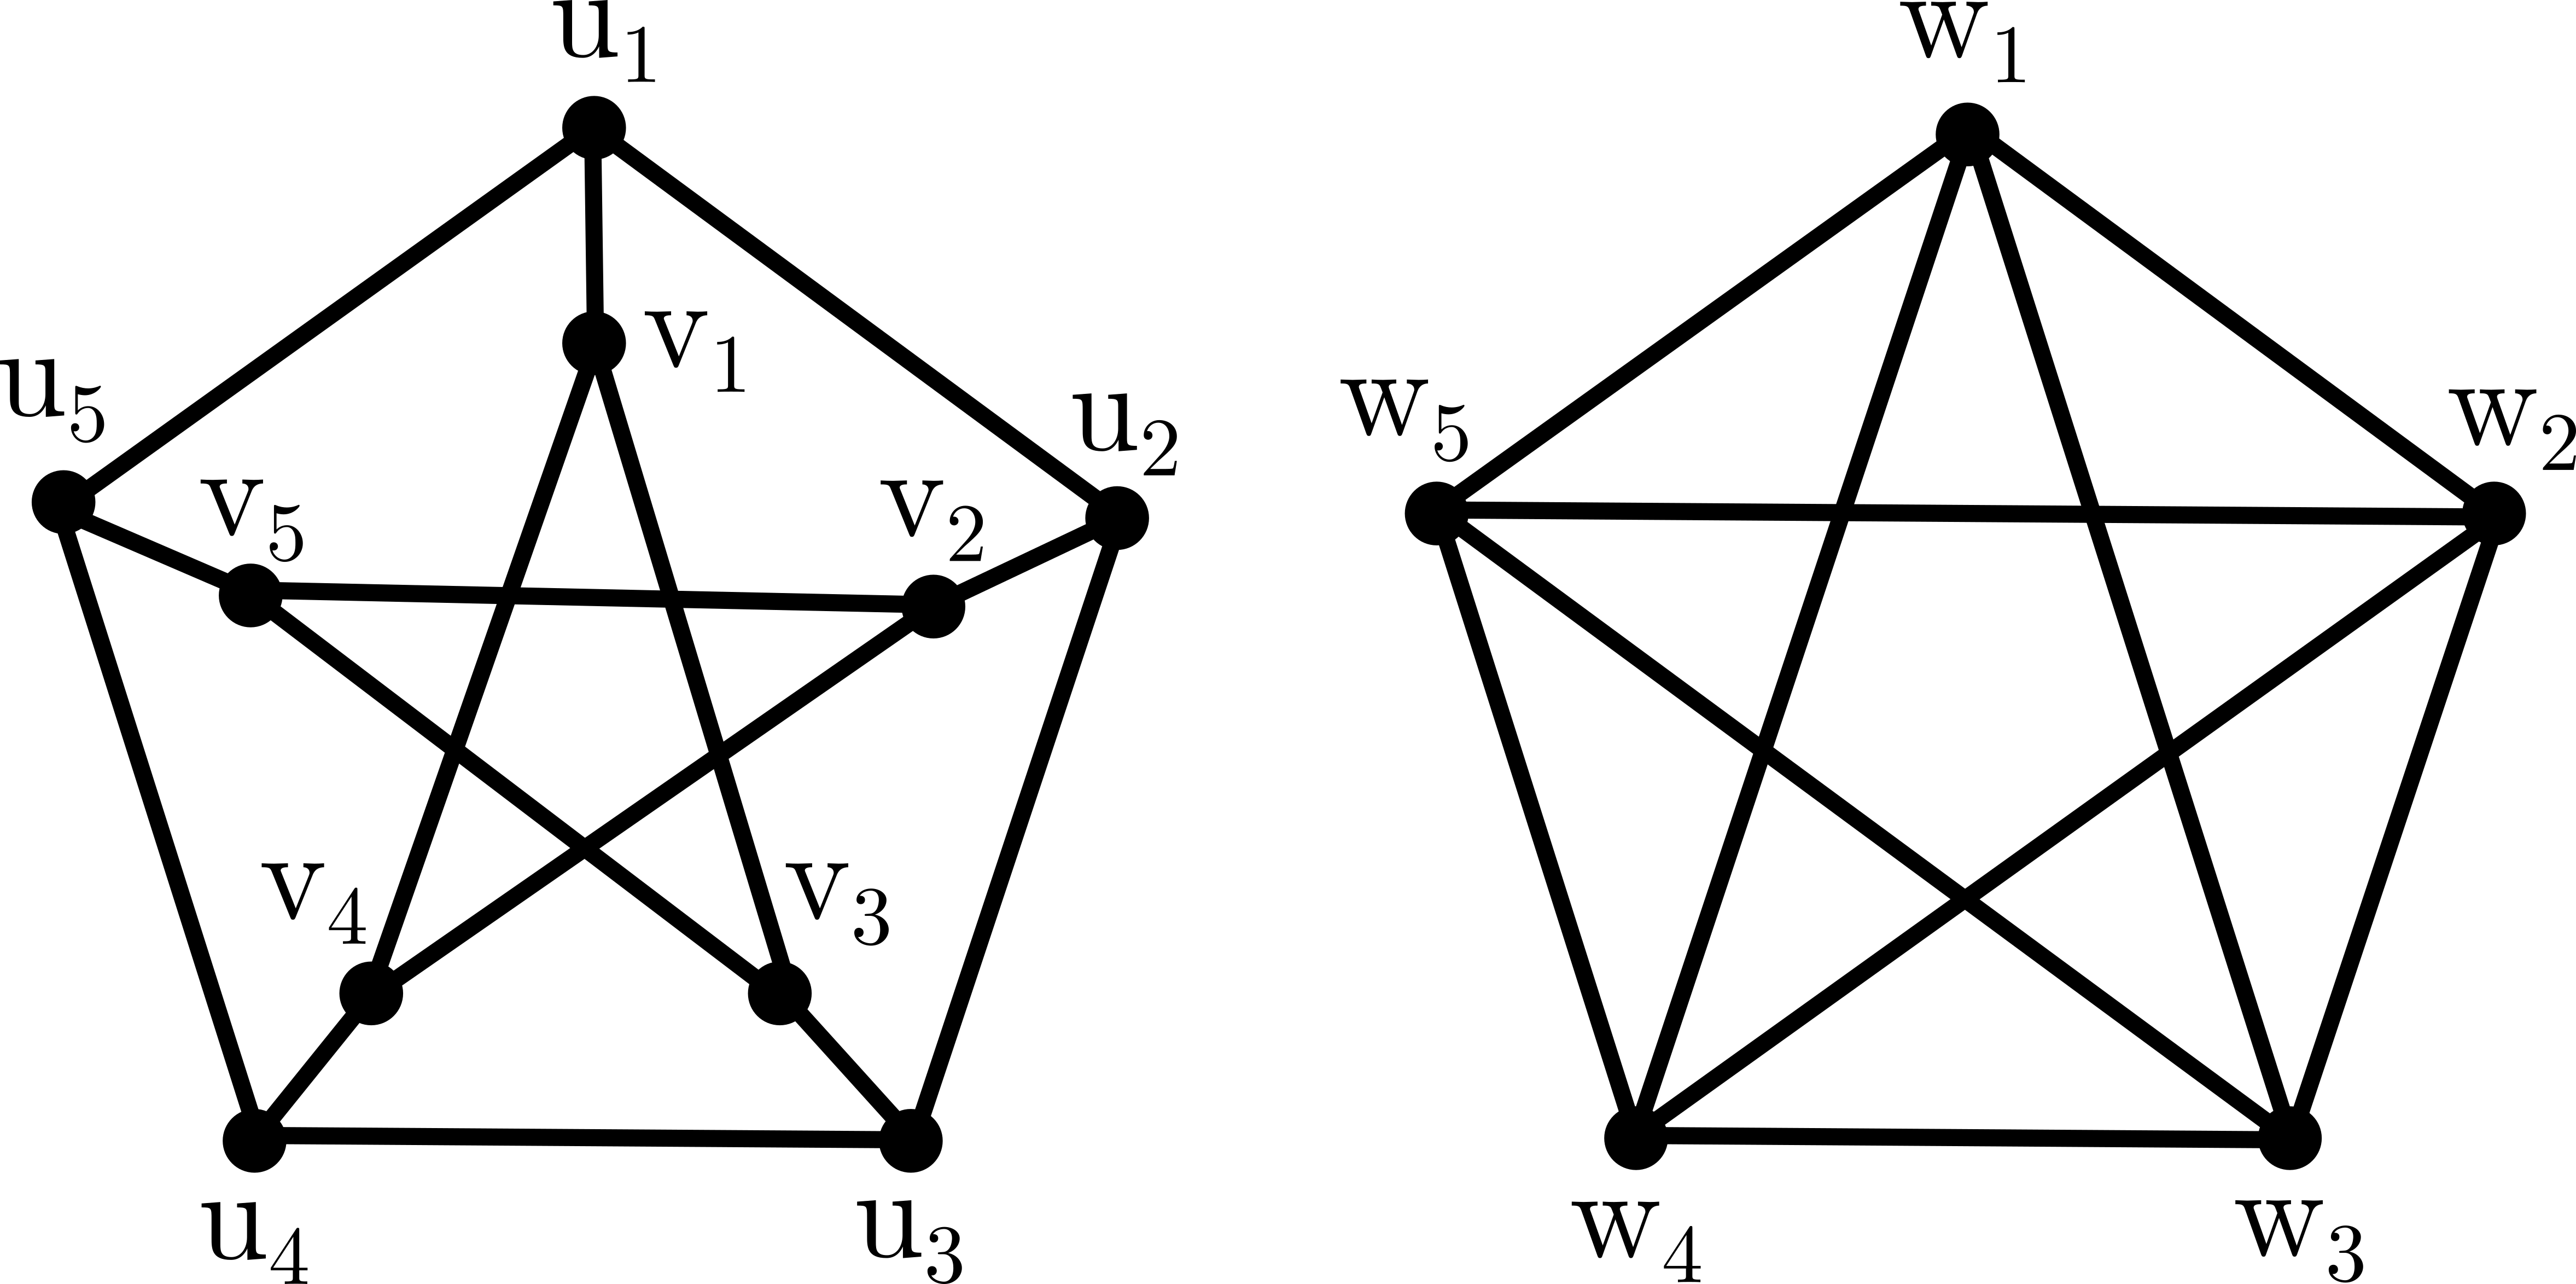
\includegraphics[width=0.75\textwidth]{images/graph-contraction-example.png}
    \end{figure}

    Граф Петерсена (левый граф) стягивается к \(K_5\) (правый граф) в результате стягивания в новую вершину \(w_i\) любого из пяти ребер \(u_i v_i\), соединяющих пятиугольник с пентаграммом.
\end{example*}

\begin{theorem*}
    Граф планарен тогда и только тогда, когда у него нет подграфов, стягиваемых к \(K_5\) и к \(K_{3, 3}\).
\end{theorem*}

\subsection{Обходы графов}

\subsubsection{Эйлеровы графы}

Граф, в котором найдется маршрут, начинающийся и заканчивающийся в одной вершине, и проходящий по всем ребрам графа ровно один раз, называется \textbf{эйлеровым графом}.

Последовательность вершин (может быть с повторением), через которые проходит искомый маршрут, как и сам маршрут, называется \textbf{эйлеровым циклом}.

\begin{theorem*}
    Для связного графа \(G\) эквивалентны следующие утверждения:
    \begin{enumerate}
        \item \(G\) --- эйлеров граф;
        \item каждая вершина графа \(G\) имеет четную степень;
        \item множество ребер графа \(G\) можно разбить на простые циклы.
    \end{enumerate}
\end{theorem*}

\subsubsection{Гамильтоновы графы}

Цикл, проходящий через каждую вершину графа в точности один раз, если он существует, называется \textbf{гамильтоновым}, а соответствующий граф --- \textbf{гамильтоновым графом}.

В отличие от задачи Эйлера, простого критерия гамильтоновости графа пока не известно.  Многие графы являются гамильтоновыми. В любом полом графе можно отыскать гамильтонов граф.

Количество гамильтоновых циклов в полном графе \(K_n\) равно \((n - 1)!\), где \(n\) --- количество вершин графа.

\begin{example*}
    Полный граф \(K_5\):

    \begin{figure}[H]
        \centering
        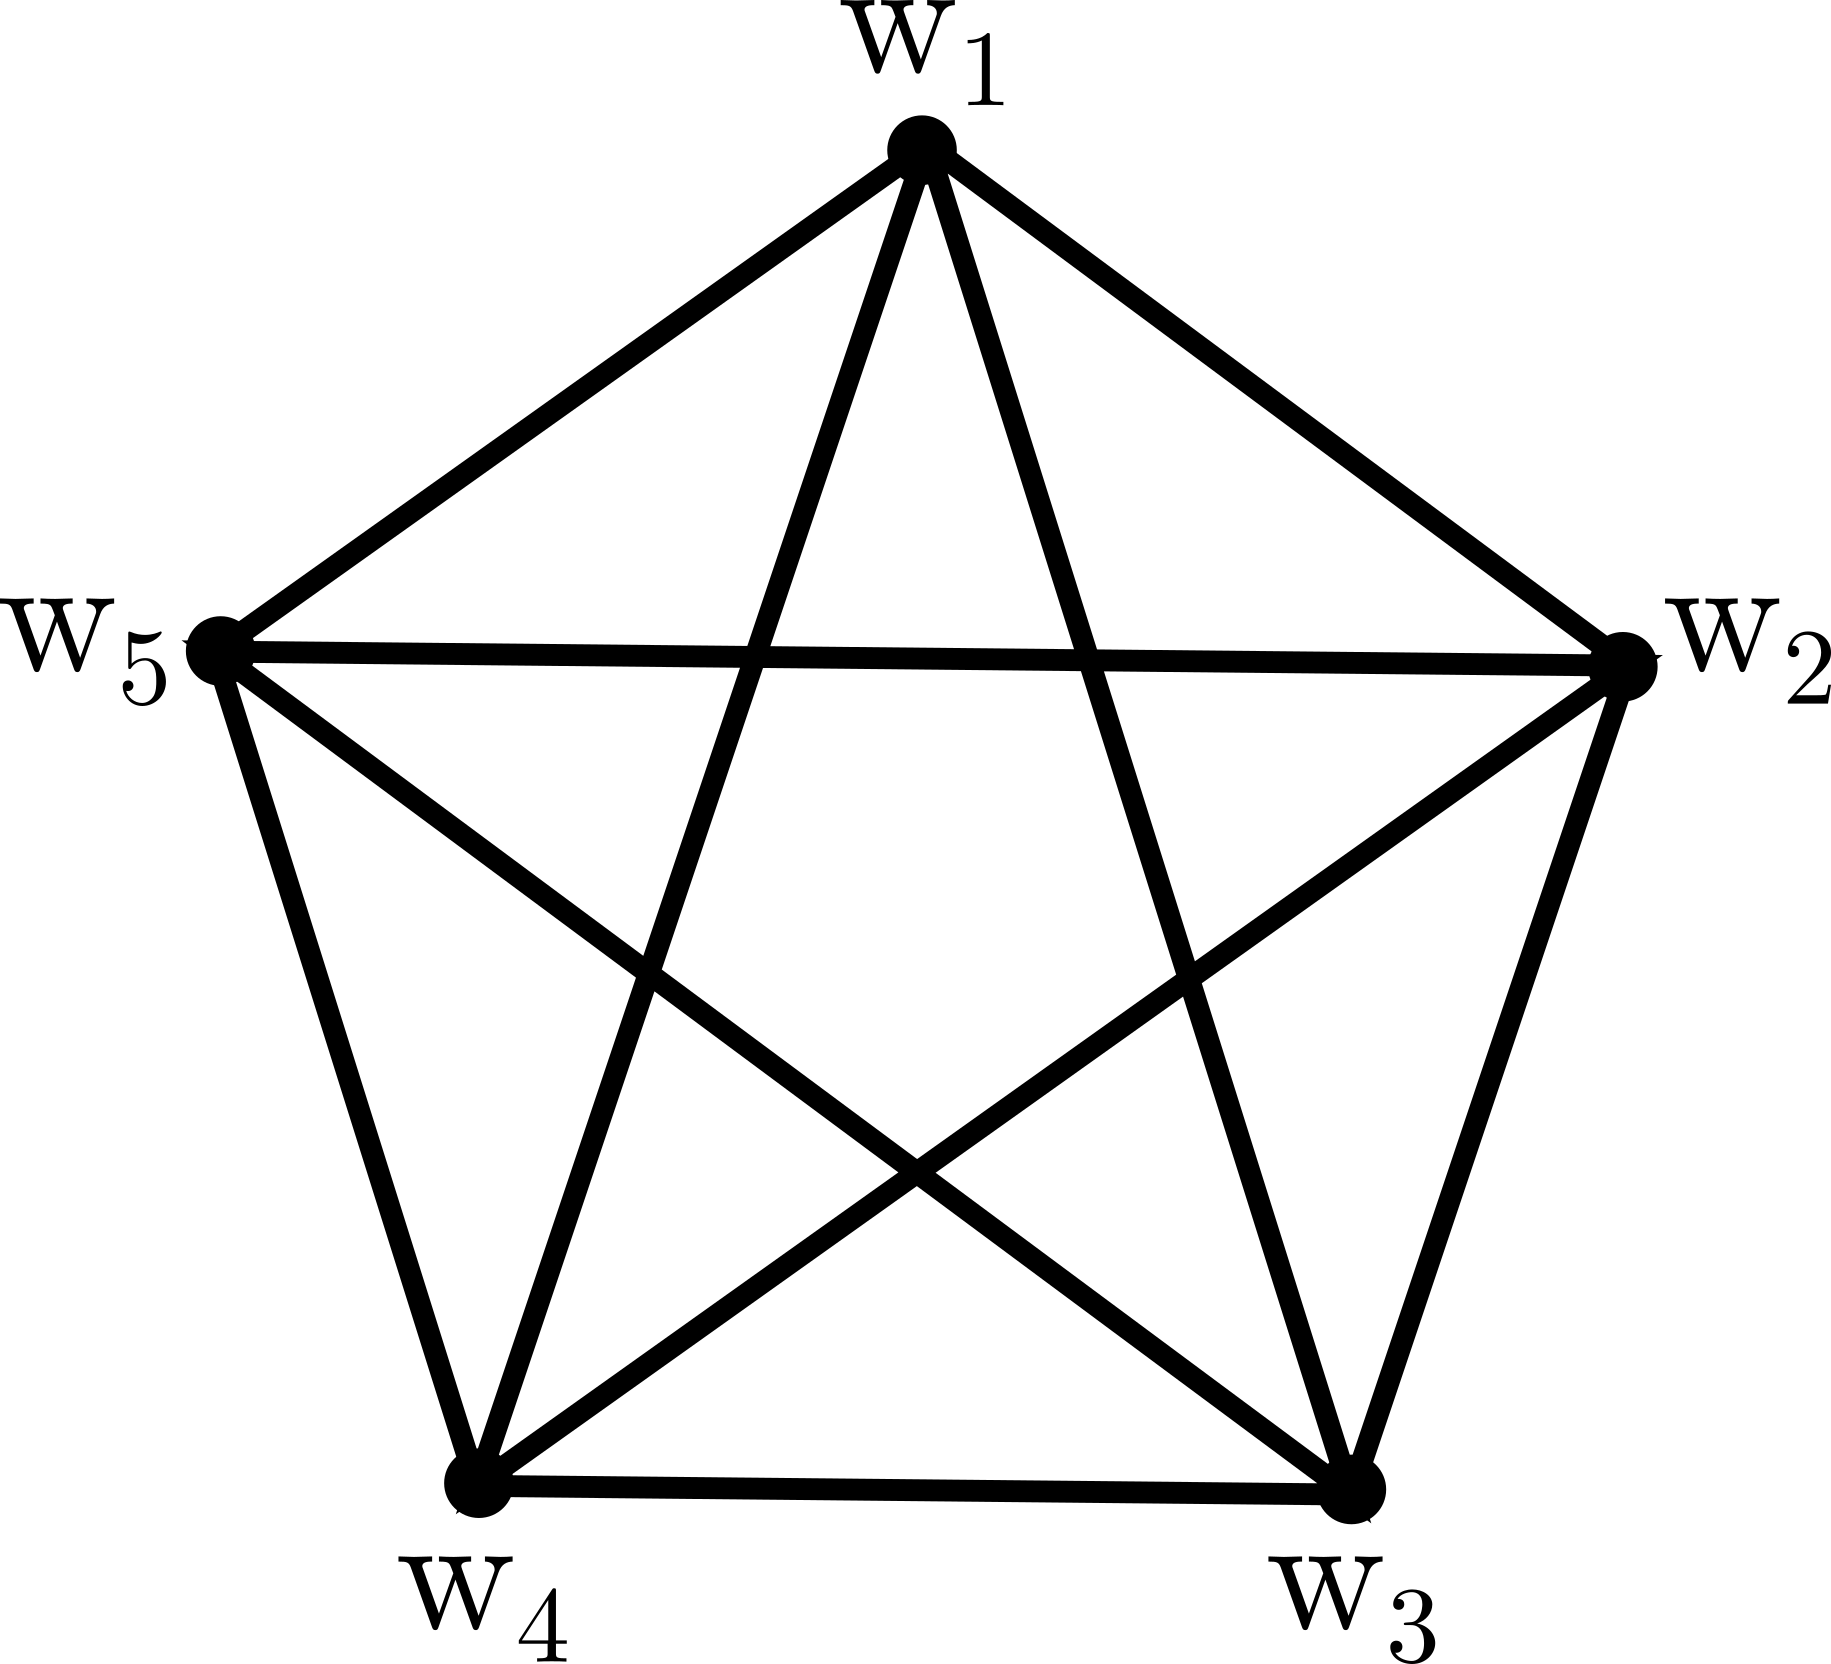
\includegraphics[width=0.45\textwidth]{images/graph-k5-example.png}
    \end{figure}

    В данном случае \(4 \cdot 3 \cdot 2 = 24\) циклов. Поскольку каждый цикл можно проходить как в одном направлении, так и в другом, то реально в графе есть только 12 разных гамильтоновых циклов.
\end{example*}

Гамильтоновы графы применяются для моделирования многих практических задач. Основой всех задач является \textbf{задача коммивояжера}, которая формулируется следующим образом: \textit{коммивояжер должен совершить поездку по городам и вернуться обратно, побывав в каждом городе ровно один раз, сведя при этом затраты на передвижения к минимуму}.

\begin{theorem*}
    Пусть \(G\) имеет \(n \geq 3\) вершин. Если для всякого \(k: 1 \leq k < \dfrac{n - 1}{2}\) число вершин со степенями, не превосходящими \(k\), меньше чем \(k\), и для нечетного \(n\) число вершин степени \(\dfrac{n - 1}{2}\) не превосходит \(\dfrac{n - 1}{2}\), то граф \(G\) является гамильтоновым графом.
    \begin{consequence}[теорема Оре]
        Если \(n \geq 3\) и \(\deg n + \deg v \geq n\) для любой пары \(n\) и \(v\) несмежных вершин графа \(G\), то граф \(G\) является гамильтоновым графом.
    \end{consequence}
    \begin{consequence}[теорема Дирака]
        Если \(n > 3\) и \(\deg v \geq \dfrac{n}{2}\) для любой вершины \(v\) графа \(G\), то граф \(G\) является гамильтоновым графом.
    \end{consequence}
\end{theorem*}

\begin{theorem*}
    Если \(G\) есть \((n, m)\)-граф, у которого \(n \geq 3\) и \(m \geq \dfrac{n^2 - 3n + 6}{2}\), то \(G\) --- гамильтонов граф.
\end{theorem*}

\begin{example*}
    Эйлеровы и неэйлеровы, гамильтоновы и негамильтоновы графы:
    \begin{figure}[H]
        \centering
        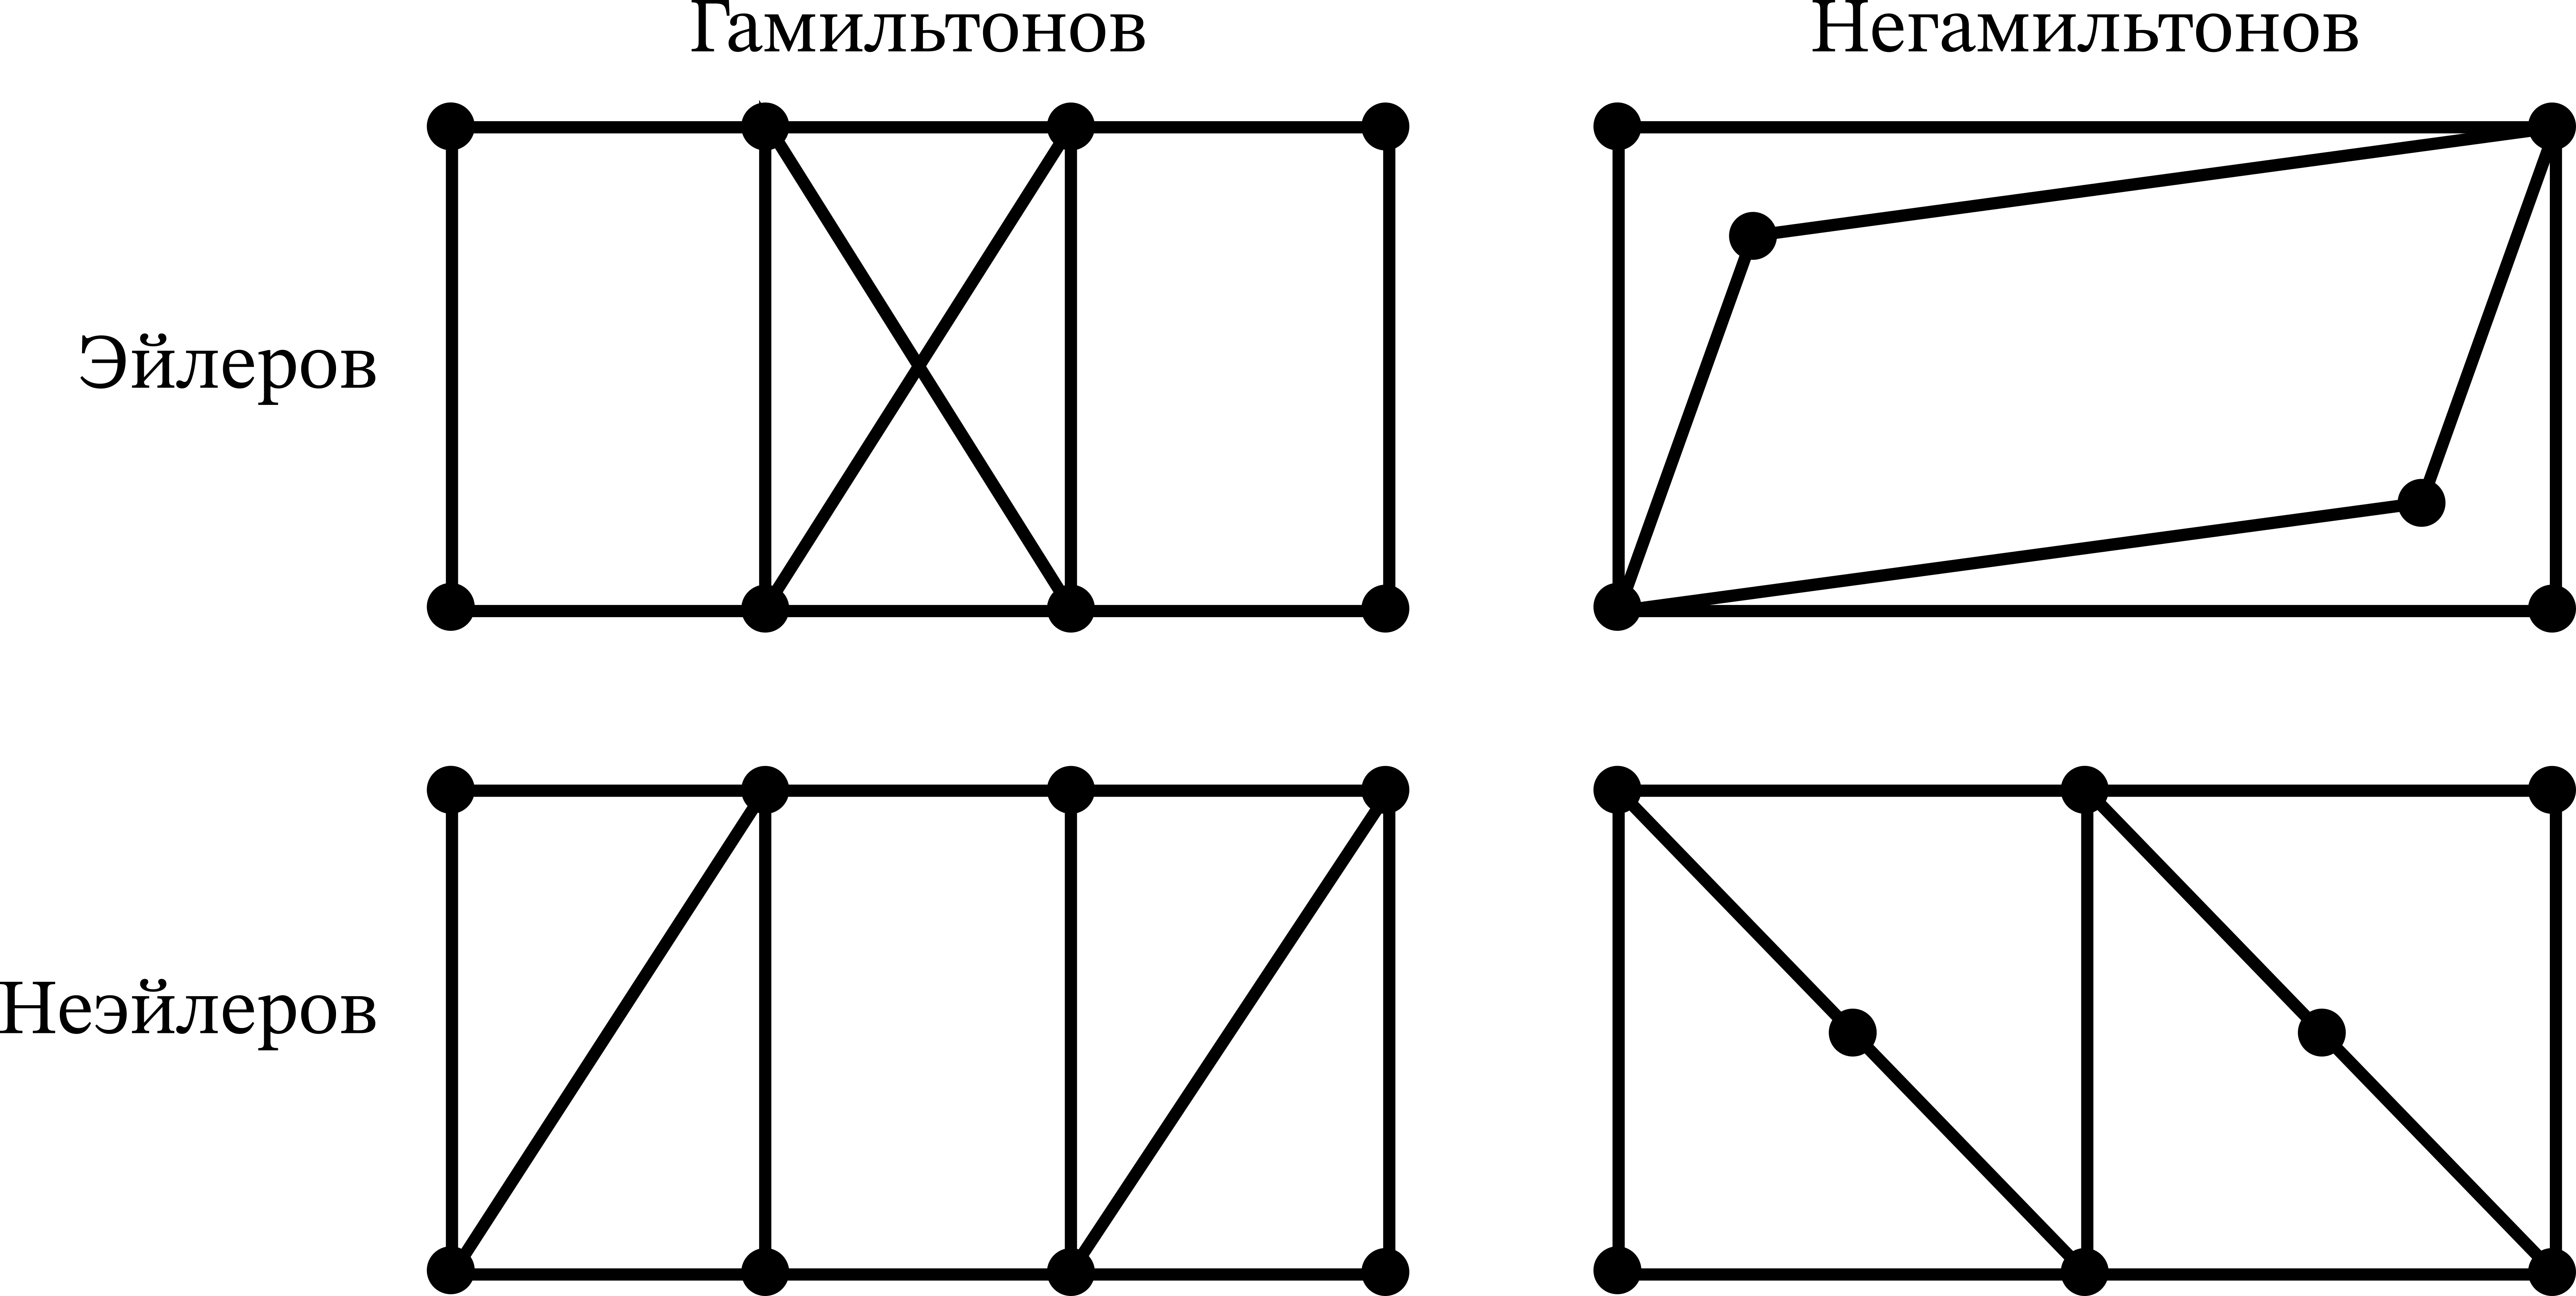
\includegraphics[width=0.9\textwidth]{images/hamiltonian-euler-example.png}
    \end{figure}
\end{example*}

\subsection{Операции над графами}

\textbf{Объединение} графов \(G_1 (V_1, E_1)\) и \(G_2 (V_2, E_2)\) обозначается
\[
    G_1 \cup G_2
    \; \text{при условии} \;
    V_1 \cap V_2 = \varnothing,
\]
и дает граф \(G (V, E)\), где
\[
    V = V_1 \cup V_2,
    \quad
    E = E_1 \cup E_2.
\]

\textbf{Удаление вершины} \(v\) из графа \(G_1 (V_1, E_1)\) обозначается
\[
    G_1 (V_1, E_1) - v
    \; \text{при условии} \;
    v \in V_1
\]
и дает граф \(G_2 (V_2, E_2)\), где
\[
    V_2 = V_1 \setminus \{v\},
    \quad
    E_2 = E_1 \setminus \{e = \{v_1, v_2\} \mid v_1 = v \lor v_2 = v\}.
\]

\textbf{Удаление ребра} \(e\) из графа \(G_1 (V_1, E_1)\) обозначается
\[
    G_1 (V_1, E_1) - e
    \; \text{при условии} \;
    e \in E_1
\]
и дает граф \(G_2 (V_2, E_2)\), где
\[
    V_2 = V_1,
    \quad
    E_2 = E_1 \setminus \{e\}.
\]

\textbf{Добавление вершины} \(v\) в граф \(G_1 (V_1, E_1)\) обозначается
\[
    G_1 (V_1, E_1) + v
    \; \text{при условии} \;
    v \notin V_1
\]
и дает граф \(G_2 (V_2, E_2)\), где
\[
    V_2 = V_1 \cup \{v\},
    \quad
    E_2 = E_1.
\]

\textbf{Добавление ребра} \(e\) в граф \(G_1 (V_1, E_1)\) обозначается
\[
    G_1 (V_1, E_1) + e
    \; \text{при условии} \;
    e \notin E_1
\]
и дает граф \(G_2 (V_2, E_2)\), где
\[
    V_2 = V_1,
    \quad
    E_2 = E_1 \cup \{e\}.
\]

\textbf{Стягивание ребра} \(e = uv\) графа \(G_1 (V_1, E_1)\) обозначается
\[
    G_1 (V_1, E_1) \cdot e(G_1 (V_1, E_1) \setminus e)
    \; \text{при условии} \;
    e \in E_1 (\{u, v\} \in V_1
\]
и дает граф \(G_2 (V_2, E_2)\), полученный из графа \(G_1 (V_1, E_1) - u - v\) добавлением новой вершины \(w\) (\(w \notin V_1\)), которая будет смежна в графе \(G_1 (V_1, E_1) \cdot e\) со всеми вершинами графа \(G_1 (V_1, E_1)\), смежными в \(G_1 (V_1, E_1)\) хотя бы с одной из вершин \(u\) или \(v\) (обозначение \(w = u \cdot v\)).
